\documentclass[letterpaper]{article}
\usepackage[preprint]{aaai2027}
\usepackage[hyphens]{url}
\usepackage{graphicx}
\urlstyle{rm}
\def\UrlFont{\rm}
\usepackage{natbib}
\usepackage{caption}
\frenchspacing
\usepackage{booktabs}
\usepackage{array}
\usepackage{amsmath,amssymb}
\usepackage{listings}
\lstset{basicstyle=\footnotesize\ttfamily,breaklines=true,breakatwhitespace=false,columns=fullflexible,keepspaces=true,showstringspaces=false}
\providecommand{\tightlist}{}
\pdfminorversion=5
\pdfinfo{/TemplateVersion (2027.1)}
\setcounter{secnumdepth}{2}
\DeclareUnicodeCharacter{2212}{\ensuremath{-}}
\DeclareUnicodeCharacter{00D7}{\ensuremath{\times}}
\DeclareUnicodeCharacter{00F7}{\ensuremath{\div}}
\DeclareUnicodeCharacter{2264}{\ensuremath{\leq}}
\DeclareUnicodeCharacter{2248}{\ensuremath{\approx}}
\DeclareUnicodeCharacter{2192}{\ensuremath{\rightarrow}}
\DeclareUnicodeCharacter{2190}{\ensuremath{\leftarrow}}
\DeclareUnicodeCharacter{2194}{\ensuremath{\leftrightarrow}}
\DeclareUnicodeCharacter{2193}{\ensuremath{\downarrow}}
\DeclareUnicodeCharacter{0394}{\ensuremath{\Delta}}
\DeclareUnicodeCharacter{03C7}{\ensuremath{\chi}}
\DeclareUnicodeCharacter{03B1}{\ensuremath{\alpha}}
\DeclareUnicodeCharacter{03BB}{\ensuremath{\lambda}}
\DeclareUnicodeCharacter{03BA}{\ensuremath{\kappa}}
\DeclareUnicodeCharacter{2227}{\ensuremath{\wedge}}
\DeclareUnicodeCharacter{00B7}{\ensuremath{\cdot}}
\DeclareUnicodeCharacter{207B}{\textsuperscript{-}}
\DeclareUnicodeCharacter{2070}{\textsuperscript{0}}
\DeclareUnicodeCharacter{00B9}{\textsuperscript{1}}
\DeclareUnicodeCharacter{00B2}{\textsuperscript{2}}
\DeclareUnicodeCharacter{00B3}{\textsuperscript{3}}
\DeclareUnicodeCharacter{2074}{\textsuperscript{4}}
\DeclareUnicodeCharacter{2075}{\textsuperscript{5}}
\DeclareUnicodeCharacter{2076}{\textsuperscript{6}}
\DeclareUnicodeCharacter{2077}{\textsuperscript{7}}
\DeclareUnicodeCharacter{2078}{\textsuperscript{8}}
\DeclareUnicodeCharacter{2079}{\textsuperscript{9}}
\lstset{literate={─}{{-}}1 {│}{{|}}1 {┌}{{+}}1 {┐}{{+}}1 {┘}{{+}}1 {└}{{+}}1 {►}{{$\triangleright$}}1 {◄}{{$\triangleleft$}}1 {▼}{{$\triangledown$}}1 {→}{{$\rightarrow$}}1 {↓}{{$\downarrow$}}1 {≤}{{$\leq$}}1 {∧}{{$\wedge$}}1 {…}{{\ldots}}1 {×}{{$\times$}}1 {—}{{\textemdash}}1 {–}{{\textendash}}1 {−}{{\ensuremath{-}}}1 {÷}{{\ensuremath{\div}}}1 {≈}{{\ensuremath{\approx}}}1 {←}{{\ensuremath{\leftarrow}}}1 {↔}{{\ensuremath{\leftrightarrow}}}1 {Δ}{{\ensuremath{\Delta}}}1 {χ}{{\ensuremath{\chi}}}1 {α}{{\ensuremath{\alpha}}}1 {λ}{{\ensuremath{\lambda}}}1 {κ}{{\ensuremath{\kappa}}}1 {·}{{\ensuremath{\cdot}}}1 {⁻}{{\textsuperscript{-}}}1 {⁰}{{\textsuperscript{0}}}1 {¹}{{\textsuperscript{1}}}1 {²}{{\textsuperscript{2}}}1 {³}{{\textsuperscript{3}}}1 {⁴}{{\textsuperscript{4}}}1 {⁵}{{\textsuperscript{5}}}1 {⁶}{{\textsuperscript{6}}}1 {⁷}{{\textsuperscript{7}}}1 {⁸}{{\textsuperscript{8}}}1 {⁹}{{\textsuperscript{9}}}1}
\title{Spend It Together or Spend It Big? Quantized Monoliths versus Full-Precision Specialist Teams for Local Financial Document Reasoning under Fixed Workstation Memory}
\author{Mutasim ur Rehman and Ahmad Raza}
\affiliations{Project Agere}
\begin{document}
\maketitle
\begin{abstract}
\textbf{Background.} Banks, lenders and funds that may not send client files to cloud language-model APIs typically deploy a single, aggressively quantized model on an analyst workstation. An alternative is to split the same memory across several smaller, full-precision ``specialist'' models (a multi-agent system). Whether that alternative is better when memory and generation budgets are actually held equal has not been measured on financial document reasoning.

\textbf{Methods.} We compare complete deployment recipes, a single-agent system (SAS) built on one larger 4-bit model and a multi-agent system (MAS) built on several resident 16-bit models, under a fixed process-tree resident-memory (RSS) ceiling and a fixed generated-token ceiling, on CPU-only commodity hardware. The primary experiment (nominal 16 GB tier) pairs Qwen2.5-14B-Instruct Q4\_K\_M (SAS) with a resident Qwen2.5-1.5B/3B/0.5B F16 team (MAS) on 160 numerical questions from 50 held-out FinQA company-year reports (36 companies), under an 11.5 GB application ceiling, a 4,096-token context and a 2,048-token generation budget per question. Both arms share the same evidence packets, deterministic program executor and review gate. Three prompt profiles (primary, direct control, repair ablation) give 960 audited outputs. Each output is classified as correct delivered, wrong delivered or withheld under two numerical scoring conventions. Inference uses whole-report cluster bootstrap (10,000 resamples), company-cluster sensitivity, cluster sign-flip and cluster-adjusted McNemar tests with Holm correction, Bowker and Stuart--Maxwell tests on the 3×3 outcome-transition tables, and conditional formal bounds, under a stated set of testing standards. Two earlier 8 GB evidence regimes, a 175-case synthetic KYC/credit study and a 15-configuration adapted FinQA development programme, are reported separately and not pooled.

\textbf{Results.} In the primary profile SAS delivered 78 correct and 48 wrong answers and withheld 34. MAS delivered 5 correct and 3 wrong and withheld 152. MAS minus SAS was −45.6 percentage points (pp) in correct delivery (report-cluster 95\% CI −53.9 to −36.6), −28.1 pp in wrong delivery (−37.1 to −20.1) and +73.8 pp in withholding. All four primary correct/wrong contrasts had Holm-adjusted p ≤ 6.1×10⁻⁵ under both cluster-level tests, and the 3×3 outcome-transition table was strongly asymmetric (Bowker Q = 119, 3 df). MAS never delivered a correct answer that SAS missed, and was better than SAS on none of the 50 reports. Conditional precision was nearly identical (61.9\% vs 62.5\%) at radically different coverage (78.8\% vs 5.0\%). A stage decomposition places the MAS bottleneck in candidate production, not review: only 10 of 160 MAS drafts were executable, so no accept/reject gate could have delivered more than 5 correct answers. The reasoning-plus-demonstration prompt bundle improved both arms relative to direct control. Repair added 1.25--1.95 inference hours and produced no Pareto improvement. Despite fewer parameters, MAS used more peak RSS (10.93 vs 10.06 GB) and 3.3 times more inference time per correct answer. In the historical 8 GB synthetic study, the 7B Q4 monolith also dominated (valid JSON 100\% vs 63.4\%; claim-level grounding 84.4\% vs 36.3\%).

\textbf{Conclusions.} Under matched memory and token ceilings on these tasks, spending memory on one larger quantized model gave far more useful answers than splitting it across a resident full-precision team. The team's lower error count came almost entirely from abstention. The evidence supports a bounded empirical claim about these deployment recipes, together with a coverage-aware evaluation framework. It establishes neither a universal architecture law, a pure precision effect, a causal RAM-scaling curve nor regulatory readiness. Two historical swap events mean the 16 GB accuracy evidence is complete and audited but is not an uninterrupted no-swap deployment certification.
\end{abstract}
\textbf{Manuscript date:} 30 October 2026 · \textbf{Status:} complete research paper for the evaluated tiers at or below 16 GB. The 32 GB tier was not run and is reported only as future work; no 32 GB result is claimed or extrapolated.

\textbf{Keywords:} local LLM deployment · multi-agent systems · post-training quantization · resource parity · financial question answering · selective prediction · cluster bootstrap · regulated finance
\section{Introduction}\label{introduction}

\subsection{Motivation}\label{motivation}

Know-your-customer (KYC) onboarding, credit-memo drafting and mortgage origination checks are document-heavy, numerically exacting and legally sensitive. Supervisory and data-protection regimes (for example FINRA Regulatory Notice 24-09, SEC Rule 17a-4 record-keeping, GDPR, the EU Digital Operational Resilience Act and State Bank of Pakistan AML/CFT regulations) push institutions to keep client data on premises. In practice the inference hardware is often the analyst's own workstation: 8--16 GB of system RAM, a commodity CPU, and no datacenter GPU.

Practitioners facing that envelope usually pick the largest open-weight model that fits after 4-bit post-training quantization and run it through a local runtime such as \path|llama.cpp| or Ollama. The multi-agent literature suggests an alternative: decompose the workflow into roles (extract, draft, verify) and serve each role with a smaller model kept at native 16-bit precision. The question this paper answers is simple to state and has not been measured on financial document reasoning under real resource parity:

\begin{quote}
\textbf{Research question.} When both systems must fit the same host-adjusted process-tree RSS ceiling and the same generated-token budget, does a team of smaller full-precision specialist models outperform a single larger quantized model on local financial document reasoning?
\end{quote}

\subsection{Status quo}\label{status-quo}

The current default, a quantized monolith, rests on three observations from prior work. Within a fixed GPU memory budget, larger quantized models can outperform smaller FP16 models, although the trade-offs vary by model family (Stuhlmann et al., 2025, Bench360). Multi-agent advantages often disappear once test-time compute is equalized (Tran \& Kiela, 2026). Multi-agent pipelines fail in characteristic ways, grouped as system-design issues, inter-agent misalignment and task-verification failures (Cemri et al., 2025). Against that, quantization has been reported to amplify the failure modes an agent already shows at full precision, such as tool-name hallucination and wrong-entity arguments, while leaving headline scores flat (Jang et al., 2026). An independent full-precision verifier role is meant to catch exactly that kind of failure. No prior study we located holds physical process memory and generation budget equal while comparing these two deployment styles on financial documents (Section 3.7).

\subsection{Contributions}\label{contributions}

\begin{enumerate}
\def\labelenumi{\arabic{enumi}.}
\tightlist
\item
  \textbf{A resource-matched empirical comparison.} We report a completed, fully audited head-to-head comparison of a 14B Q4 monolith against a resident 1.5B/3B/0.5B F16 team under an 11.5 GB process-tree RSS ceiling and a 2,048-token generation budget, on 160 held-out financial numerical questions. We keep every case, including all withheld outputs, in every denominator.
\item
  \textbf{A coverage-aware evaluation lens.} We show why ``fewer wrong answers'' is not an improvement on its own. We report correct, wrong and withheld outcomes jointly under two numerical scoring conventions, with dependence-aware uncertainty at report and company level. Explicit testing standards and a full numerical test battery accompany each test, with its theoretical justification, including bounds showing how far case-level p-values overstate clustered evidence.
\item
  \textbf{A stage decomposition that locates the bottleneck.} We use an exact identity, correct = executable × correct-given-executable × gate acceptance, together with a fixed-candidate gate bound. They show that the team's deficit arises at candidate production, so no better reviewer could have rescued it.
\item
  \textbf{Negative ablations reported in full.} The prompt bundle helps both arms. The tested repair policy costs 1.25--1.95 extra hours with no Pareto improvement.
\item
  \textbf{A transparent resource audit.} It covers sampled RSS traces, two retained swap failures, checkpoint-replay continuation and kernel-level swap prevention. It also documents platform pitfalls at 8 GB (memory-mapped double counting on Windows and corrupted 4-bit KV caches on CPU).
\item
  \textbf{Reproducible artefacts.} We release 960 case-level rows, report-level tables, paired contrasts, stage costs, scripts that re-verify input hashes, and 26 figures (9 produced for this paper; 20 are reproduced in this document).
\end{enumerate}

\subsection{Scope}\label{scope}

All results are for nominal tiers at or below 16 GB. A 32 GB configuration (Qwen2.5-32B Q4\_K\_M versus a resident 3B/7B/0.5B F16 team under a 25.6 GB ceiling) was specified and its weights staged, but it was not executed. We do not report or extrapolate it. We compare whole recipes. Model size, precision, number of roles and internal prompts differ jointly between arms, so the study is not a factorial isolation of architecture or precision.

\section{Background}\label{background}

\subsection{Workstation memory as the binding constraint}\label{workstation-memory-as-the-binding-constraint}

On a CPU-only workstation the resident set must hold all model weights, KV caches, runtime buffers and the controller process. Under the RAM Utilization Parity Protocol (RUPP) used throughout this project, at least 20\% of physical RAM is reserved for the operating system and background compliance agents, giving nominal caps of 6.4, 12.8 and 25.6 GB on 8, 16 and 32 GB hosts. The cap is lowered further when measured idle memory plus a 1 GB margin requires it:

\[M_{\text{job}} = \min\big(0.8\,M_{\text{tier}},\; M_{\text{host}} - M_{\text{idle}} - 1\,\text{GB}\big).\]

The 16 GB evaluation host exposed 15.44 GB to Linux. After an earlier 12.49 GB attempt failed its pre-inference reserve check, the study adopted a fixed \textbf{11.5 GB application ceiling} that includes the controller, plus a separate 1 GB host reserve (Section 5.2).

\subsection{Quantization and storage arithmetic}\label{quantization-and-storage-arithmetic}

GGUF \path|Q4_K_M| stores most weights at roughly 4.5--5 effective bits per element, including block scales. F16 uses 16 bits. A 14B model at Q4\_K\_M occupies 8.99 GB on disk, while the 1.5B + 3B + 0.5B F16 team occupies 10.27 GB. Fewer total parameters therefore do not imply a smaller footprint when precision differs. Proposition 6 (Section 8) states this formally.

\subsection{Selective answering}\label{selective-answering}

A system that may abstain trades \textbf{coverage}, the fraction of questions answered, against \textbf{risk}, the error rate among answers delivered (El-Yaniv \& Wiener, 2010). In regulated workflows a withheld answer is routed to a human and a wrong delivered answer may propagate into a filing. Both matter, so neither accuracy alone nor precision alone is an adequate summary. We report all three delivery states.

\section{Literature Review}\label{literature-review}

The review combines a 9-paper foundational corpus (Phase 1), a 10-paper extended corpus (Phase 2) and a later closest-work audit carried out during development to constrain novelty claims. It is organized by theme, and each theme ends with what remains unresolved for our setting.

\subsection{Test-time compute parity}\label{test-time-compute-parity}

Tran \& Kiela (2026) showed that on multi-hop reasoning (FRAMES and MuSiQue), single-agent systems consistently match or outperform multi-agent systems when reasoning tokens are held constant. They argued, via the data-processing inequality, that natural-language handoffs without fresh evidence are lossy. Wang et al.~(2024) similarly argued for budget-aware evaluation, finding that complex reasoning strategies often beat simpler baselines because they are allocated more compute, not because of algorithmic ingenuity. \emph{Gap:} compute is modelled as tokens only. Physical memory, quantization and tool-grounded document tasks are absent.

\subsection{When teams help: scaling and tool access}\label{when-teams-help-scaling-and-tool-access}

Żywot et al.~(2026) found that gains were driven primarily by orchestrator capacity rather than sub-agent capacity, and that an 8B multi-agent system matched a 32B single agent on GAIA (23.0 vs 23.0) and outperformed it on AIME (55.0 vs 45.0), even when the single agent had direct access to the same tools. Kim et al.~(2025) related agent scaling to task structure: relative to a single-agent baseline, multi-agent performance ranged from +80.8\% on decomposable financial reasoning to −70.0\% on sequential planning, and independent (uncoordinated) agents amplified trace-level errors far more than centrally coordinated ones. MetaGPT (Hong et al., 2024) popularized role-specialized orchestration, and later work studied evolving orchestration (Dang et al., 2025), decentralized evolutionary coordination (AgentNet; Yang et al., 2025) and benchmarking of multi-agent collaboration against conventional methods on medical tasks (MedAgentBoard; Zhu et al., 2025). \emph{Gap:} these studies assume elastic cloud memory, and none fixes resident RAM across arms.

\subsection{How multi-agent systems fail}\label{how-multi-agent-systems-fail}

Cemri et al.~(2025, MAST) catalogued 1,600+ traces into 14 failure modes in three categories: system design, inter-agent misalignment and task verification. Jamshidi et al.~(2026) measured hallucination propagation through agent chains and found net attenuation of the hallucination score in 3-agent chains, alongside a small decline in factual accuracy. Singh \& Pawar (2026) modelled propagation in a 4-agent financial-analysis pipeline on FinanceBench as a Markov process: detection fell from 72.0\% at the first stage to 50.9\% at the fourth, and boundary verification gates cut hallucination survival from 58.4\% to 16.2\% compared with end-of-pipeline checking. Wan et al.~(2025, MAMM-Refine) found critique-guided reranking more effective than free revision for faithfulness. Estornell et al.~(2025, ACC-Collab), Li et al.~(2025) and Sun et al.~(2025, Collab-Overcooked) studied learned actor--critic collaboration, role differentiation and shortcomings in active collaboration and adaptation. \emph{Gap:} these studies use cloud or API models without memory ceilings, and only one (Singh \& Pawar) uses financial documents. In our pipeline every role also sees the source evidence, not only the upstream message, so propagation estimates from message-only chains do not transfer directly (Section 8, ``Nonidentification'').

\subsection{Quantization in agentic settings}\label{quantization-in-agentic-settings}

AWQ (Lin et al., 2024) outperforms round-to-nearest and GPTQ 4-bit quantization across 7B--70B models, and SpinQuant (Liu et al., 2025) narrows the gap to full precision to 2.9 points on LLaMA-2 7B with 4-bit weights, activations and KV cache. MobileLLM (Liu et al., 2024) targets sub-billion-parameter on-device models, and BFCL (Patil et al., 2025) standardized function-calling evaluation. Jang et al.~(2026) reported that quantization can look free on the standard metric while amplifying, by up to 2.5×, the failure an agent already shows at full precision, mainly tool-name hallucination and wrong-entity arguments. Malformed arguments were rare (≈0.1\%). Quantigence (Alquwayfili, 2025) ran a multi-agent framework on consumer hardware (an 8 GB GPU) using 4-bit quantization and serialized execution. \emph{Gap:} no study pits a quantized monolith against a native-precision specialist team under the same RSS budget on CPU.

\subsection{Local inference and financial reasoning}\label{local-inference-and-financial-reasoning}

Bench360 (Stuhlmann et al., 2025) profiled local inference across memory, latency, energy and quality on single 24 GB GPUs. It compared smaller FP16 models with larger quantized models from the same family (for Qwen2.5: 7B FP16, 14B INT8 and 32B INT4) and found that quantized larger models often scored higher but at a family-dependent system cost, with ``no universal best option''. It evaluated single models only, and did not test CPU inference. Liu et al.~(2026) compared retrieval and structured memory for financial QA with one locally hosted 8B model: structured memory helped deterministic, operand-explicit tasks and retrieval helped conversational ones. MortarBench (Toles et al., 2026) introduced mortgage-origination agent tasks. FinQA (Chen et al., 2021) established numerical reasoning over financial reports with annotated gold programs, TAT-QA/TAGOP (Zhu et al., 2021) did so for hybrid tables and text with symbolic aggregation operators, and later work showed that small models fine-tuned on financial programs can improve substantially (Phogat et al., 2024).

\subsection{Closest prior work on financial agents and verification}\label{closest-prior-work-on-financial-agents-and-verification}

A development-time audit found that most individual components of our pipeline have close precedents:

\begin{itemize}
\tightlist
\item
  financial specialist decomposition with formula planning, quantity extraction, code execution and staged checking (FinMAN / ``David vs.~Goliath'', 2025);
\item
  independent concept/period/unit binding against XBRL facts with formal (Z3) checks whose named-constraint feedback can guide repair (VeriFin, 2026);
\item
  cost-aware routing between no verification, local revision and full re-solve (BudgetVerify, 2026);
\item
  source-labelled evidence with symbol binding and deterministic operators, using Qwen2.5 1.5B/3B/7B (DCRC, 2026);
\item
  role-specific LoRA agents sharing a backbone and KV caches (LRAgent, 2026; ForkKV, 2026);
\item
  execution-trace program repair, with limited gains (Haque et al., 2025);
\item
  risk/coverage-controlled abstention (SAFER, 2026).
\end{itemize}

We therefore claim \textbf{no} novel inference algorithm. The contribution is measurement and diagnosis under a constraint those works do not impose.

\subsection{Synthesis table and remaining gap}\label{synthesis-table-and-remaining-gap}

\begin{table*}[tbp]
\centering
\setlength{\tabcolsep}{3pt}
\begin{tabular}{@{}>{\raggedright\arraybackslash}p{87.05pt}>{\raggedright\arraybackslash}p{99.33pt}>{\raggedright\arraybackslash}p{62.02pt}>{\raggedright\arraybackslash}p{73.15pt}>{\raggedright\arraybackslash}p{69.64pt}>{\raggedright\arraybackslash}p{82.80pt}@{}}
\toprule
\textbf{Strand} & \textbf{Representative work} & \textbf{Controls compute?} & \textbf{Controls physical RAM?} & \textbf{Quantized vs native team?} & \textbf{Financial documents?} \\
\midrule
Token-parity SAS vs MAS & Tran \& Kiela 2026; Wang et al. 2024 & Yes (tokens) & No & No & No \\
Small-team vs large model & Żywot et al. 2026; Kim et al. 2025 & Partly & No & No & No \\
MAS failure taxonomies & Cemri et al. 2025; Jamshidi et al. 2026; Singh \& Pawar 2026 & No & No & No & Singh \& Pawar only \\
Quantized agents & Jang et al. 2026; Quantigence 2025 & No & Partly & All-quantized only & No \\
Local inference profiling & Bench360 (Stuhlmann et al.) 2025 & n/a & Yes (GPU VRAM) & Single models only & No \\
Financial agents/verification & FinMAN 2025; VeriFin 2026; DCRC 2026; BudgetVerify 2026 & Partly (tokens/cost) & Not located & No & Yes \\
\textbf{This paper} & — & \textbf{Generated-token ceiling} & \textbf{Sampled process-tree RSS ceiling} & \textbf{Yes (Q4 monolith vs F16 team)} & \textbf{Yes (FinQA reports; synthetic KYC/credit)} \\
\bottomrule
\end{tabular}
\caption{Synthesis table and remaining gap}
\end{table*}

The gap addressed is the intersection of the columns, not any single column. Phase 2 also proposed four gaps: memory-parity, confounded baselines, quantization-hardening versus verification, and compliance-aligned metrics. Section 9.4 states how far the completed evidence closes each.

\section{Research Questions and Hypotheses}\label{research-questions-and-hypotheses}

\textbf{RQ1 (primary).} Under equal RSS and token ceilings, how do the SAS and MAS recipes compare in correct deliveries, wrong deliveries and withholding?

\textbf{RQ2.} Where in the pipeline (evidence, candidate generation, review) does any difference arise?

\textbf{RQ3.} Do the shared reasoning-plus-demonstration prompt bundle and the shared repair policy improve either arm?

\textbf{RQ4.} What are the memory, latency and cost-per-useful-answer consequences?

\textbf{H1 (prespecified, primary).} The resident F16 MAS reduces wrong deliveries \emph{without} losing correct deliveries relative to the Q4 SAS. This is the operational claim that would justify the team design.

\textbf{H2.} The primary prompt bundle (128-token analysis + two training demonstrations) improves correct delivery over direct control in each arm.

\textbf{H3.} Repair improves correct delivery without adding wrong deliveries.

\textbf{H4.} The team uses no more resident memory than the monolith (the ``fewer parameters'' intuition).

The primary endpoint set and the 16 GB primary pair were fixed before evaluation. The extended statistical battery, strata and utility analyses were added afterwards and are labelled post hoc.

\section{Methodology}\label{methodology}

\subsection{Design overview: three evidence regimes}\label{design-overview-three-evidence-regimes}

The project ran in phases: literature and gap identification, synthetic data and baseline freeze, adaptation, then tier evaluations. It produced three evidence regimes with different tasks, models and adaptation. \textbf{We never pool them into a single statistical sample or a RAM-scaling curve.}

\begin{table*}[tbp]
\centering
\setlength{\tabcolsep}{3pt}
\begin{tabular}{@{}>{\raggedright\arraybackslash}p{99.99pt}>{\raggedright\arraybackslash}p{138.55pt}>{\raggedright\arraybackslash}p{139.60pt}>{\raggedright\arraybackslash}p{107.86pt}@{}}
\toprule
\textbf{Dimension} & \textbf{Historical 8 GB} & \textbf{Redeveloped 8 GB FinQA} & \textbf{16 GB FinQA (primary)} \\
\midrule
Task & Synthetic KYC/credit packs & Public FinQA train-source numerical QA & Public FinQA dev-source numerical QA \\
Unique items & 175 test cases (+150 dev) & 52 selection + 49 reserved questions & 160 questions \\
Clustering unit & Synthetic template & 15 + 15 company-year reports & 50 reports / 36 companies \\
SAS & Qwen2.5-7B Q4\_K\_M & 7B Q4 + trained adapter & Qwen2.5-14B Q4\_K\_M, pretrained \\
MAS & 1.5B + 0.5B + 0.5B F16 & Two resident 3B Q4 instances (same base checkpoint) + role adapters & 1.5B + 3B + 0.5B F16, distinct, resident \\
Context & 2,048 & 4,096 & 4,096 \\
Memory ceiling & 6.4 GB & 6.4 GB & 11.5 GB \\
Host & Windows 11, 16.39 GB RAM (CPU model not recorded in run artefacts) & Native CPU backend & Linux 7.0, AMD Ryzen 5 8645HS, 15.44 GB \\
Causal RAM comparison? & No & No & No \\
\bottomrule
\end{tabular}
\caption{Design overview: three evidence regimes}
\end{table*}

The redevelopment followed an internal audit of the historical study. That audit found the synthetic suites rule-solvable and its narrative language (e.g., ``capacity floor'', ``Markov cascade'') stronger than the evidence. The project therefore moved to a public, program-annotated benchmark with real report text and tables. The 16 GB study froze code, inputs and runtime by hash before execution.

\begin{figure*}[tbp]
\centering
\begin{tabular}{p{238pt}p{238pt}}
\multicolumn{2}{p{488pt}}{\centering Shared, identical for both arms: question $\rightarrow$ public evidence packet (lexical IDF top-8 source units + quantity catalog A000\ldots A0nn)} \\
\midrule
SAS (one 14B Q4 model) & MAS (three resident F16 models) \\
\midrule
Analysis $\leq$128 tok & 1.5B extractor: select source IDs \\
Program JSON: ANSWER/INSUFFICIENT + steps & 3B drafter: analysis $\leq$128 tok; program JSON \\
\midrule
\multicolumn{2}{p{488pt}}{\centering Deterministic executor: copies catalog values, applies add/subtract/multiply/divide, checks spans} \\
\midrule
14B review: PASS/FAIL/UNKNOWN & 0.5B verifier: PASS/FAIL/UNKNOWN \\
\midrule
\multicolumn{2}{p{488pt}}{\centering Deliver if ANSWER $\wedge$ executable $\wedge$ PASS, else withhold (repair-ablation profile: one full re-plan + re-review)} \\
\midrule
\multicolumn{2}{p{488pt}}{\centering Score: reported-answer convention and raw-execution convention $\rightarrow$ C / W / H} \\
\end{tabular}
\end{figure*}

\subsection{Resource parity protocol}\label{resource-parity-protocol}

\textbf{Memory.} A controller samples the summed RSS and swap of the controller and all worker processes every 0.2 s. A run is invalid if RSS exceeds the ceiling or if any process-tree swap appears. The 16 GB ceiling is 11,500,000,000 bytes and includes the controller. A 1 GB host reserve plus a 100 MB launch cushion must be available before launch (12.6 GB available RAM). Sampling is not a hard cgroup RSS bound, and peaks between samples cannot be excluded.

\textbf{Context.} Engineering probes at an 8,192-token context swapped. The common context was therefore reduced to 4,096 tokens for both arms before the accuracy run. Weights and precision did not change. Neutral long-input probes then peaked at 9.98 GB (SAS) and 10.85 GB (MAS) with no swap.

\textbf{Tokens.} Each question has a 2,048 generated-token ceiling summed across all stages and roles. Equal ceilings do not mean equal FLOPs or equal actual spend; both are measured. No context or budget skips occurred in any of the six jobs.

\textbf{Runtime.} Both arms use \path|llama-cpp-python| 0.3.16 (portable AVX2 build), Python 3.12, 8 threads, \path|n_gpu_layers=0|, \path|use_mmap=False|, temperature 0 (greedy), seed 42, F16 KV cache, and a KV reset on every call.

\subsection{Systems under comparison}\label{systems-under-comparison}

\begin{table*}[tbp]
\centering
\setlength{\tabcolsep}{3pt}
\begin{tabular}{@{}>{\raggedright\arraybackslash}p{55.06pt}>{\raggedright\arraybackslash}p{136.95pt}>{\raggedright\arraybackslash}p{116.54pt}>{\raggedright\arraybackslash}p{76.29pt}>{\raggedright\arraybackslash}p{95.15pt}@{}}
\toprule
\textbf{Arm} & \textbf{Role} & \textbf{Model} & \textbf{Precision} & \textbf{GGUF bytes} \\
\midrule
SAS & All stages & Qwen2.5-14B-Instruct & Q4\_K\_M & 8,988,110,336 \\
MAS & Extractor / evidence selector & Qwen2.5-1.5B-Instruct & F16 & 3,093,669,024 \\
MAS & Drafter (analysis + program) & Qwen2.5-3B-Instruct & F16 & 6,178,316,832 \\
MAS & Verifier & Qwen2.5-0.5B-Instruct & F16 & 994,156,512 \\
 &  & \textbf{MAS total} &  & \textbf{10,266,142,368} \\
\bottomrule
\end{tabular}
\caption{Systems under comparison}
\end{table*}

Both arms are \textbf{pretrained}: the 8 GB adapters were trained for 7B/3B checkpoints and are incompatible with the 14B model. Reusing them only on one side would have confounded the comparison. All MAS models stay resident, with no backbone sharing. All arms receive the same tools: the evidence packet, quantity catalog and deterministic executor.

\subsection{Program representation and stages}\label{program-representation-and-stages}

Models never write numbers into the program. They reference catalog IDs (\path|A013|), earlier steps (\path|#0|) or whitelisted constants (\path|CONST:100|), and choose a unit (\path|number|, \path|percent|, \path|fraction|). A grammar constrains program JSON to \path!{"decision": "ANSWER"|"INSUFFICIENT", "answer_unit", "steps":[{op,left,right}]}!. The deterministic executor resolves references to source values and records source spans. The review stage sees the question, the evidence, the resolved program and the execution trace, and must judge operand relevance (row/year), operations and units, returning PASS, FAIL or UNKNOWN. A case is delivered only if the decision is ANSWER, execution is valid and the verdict is PASS. Section 7 shows actual prompts and responses.

\subsection{Prompt profiles}\label{prompt-profiles}

\begin{table*}[tbp]
\centering
\setlength{\tabcolsep}{3pt}
\begin{tabular}{@{}>{\raggedright\arraybackslash}p{92.25pt}>{\raggedright\arraybackslash}p{71.29pt}>{\raggedright\arraybackslash}p{91.38pt}>{\raggedright\arraybackslash}p{118.99pt}>{\raggedright\arraybackslash}p{106.09pt}@{}}
\toprule
\textbf{Profile} & \textbf{Analysis stage} & \textbf{Training demonstrations} & \textbf{Repair} & \textbf{Role in design} \\
\midrule
\textbf{Primary} & 128 tokens & 2 fixed & None & Prespecified primary comparison \\
Direct control & None & None & None & Bundle ablation \\
Repair ablation & 128 tokens & 2 fixed & One full re-plan + re-review after FAIL & Repair ablation \\
\bottomrule
\end{tabular}
\caption{Prompt profiles}
\end{table*}

The primary profile adds the analysis allowance and demonstrations together, so the direct-control contrast cannot separate the two. The no-repair primary was chosen before results were seen.

\subsection{Data}\label{data}

\textbf{16 GB cohort.} We took the first 50 eligible whole company-year reports, ordered by a fixed hash of report IDs, from the public FinQA development source. Reports exposed during 8 GB development were excluded, and every question in a selected report was kept (160 questions, 36 companies; 1--11 questions per report, median 3). Gold annotations were held in a separate scoring file sealed from the public packets (SHA-256 recorded). These are not the official FinQA test split, and pretraining contamination cannot be excluded. Gold reference programs comprise 104 one-step, 49 two-step and 7 three-or-more-step programs.

\textbf{8 GB FinQA cohorts.} These are 52 model-selection questions and 49 reserved questions, each drawn from 15 reports in the FinQA training source. They have no ID or report overlap with the 16 GB set.

\textbf{Synthetic KYC/credit (historical 8 GB).} \emph{Agere-KYC-Synth} (100 test cases) and \emph{Agere-Credit-Synth} (75 test cases) were generated from templates aligned with FATF and SBP practice. They include planted identity mismatches, omitted fields that require a \path|MISSING| refusal, and calculator targets (DSCR, current ratio). A 100-question FRAMES slice (Krishna et al., 2024) served as a closed-book negative control. MortarBench (90 questions) was run later, in the redeveloped 8 GB phase, as an external check (Section 6.2).

\subsection{Outcomes and metrics}\label{outcomes-and-metrics}

Every case receives exactly one state per metric: \textbf{C} (delivered and correct), \textbf{W} (delivered and wrong) or \textbf{H} (withheld). From these:

\[\begin{gathered}\text{coverage}=\frac{C+W}{N},\\ \text{precision}=\frac{C}{C+W},\\ \text{withholding}=\frac{H}{N}.\end{gathered}\]

Two numerical conventions are kept side by side, and neither was chosen after seeing results:

\begin{itemize}
\tightlist
\item
  \textbf{Reported-answer}: the prediction is normalized by its declared unit and compared to the rounded reference \path|qa.answer|.
\item
  \textbf{Raw-execution}: relative/absolute tolerance 10⁻⁵ against the reference program value \path|qa.exe_ans|, without unit normalization.
\end{itemize}

Neither is the official FinQA program-equivalence metric. Historical synthetic metrics (JSON validity, structured invention rate, claim-level citation grounding, planted-mismatch recall, refusal correctness) are reported only within that regime.

\subsection{Statistical analysis}\label{statistical-analysis}

\begin{itemize}
\tightlist
\item
  \textbf{Primary estimand.} Paired MAS − SAS difference in event rates over all 160 questions, for C and W under both metrics (four endpoints). H follows from the identity \(C+W+H=N\) and is not tested separately.
\item
  \textbf{Intervals.} Whole-report cluster bootstrap: 50 reports resampled with replacement, all questions in a report kept, question-weighted estimator, 10,000 draws, NumPy \path|default_rng(42)|, percentile intervals. Bonferroni-style 98.75\% intervals cover the four primary endpoints. Sensitivity analyses use company-cluster bootstrap (36 companies), equal-report weighting and leave-one-report-out ranges.
\item
  \textbf{Tests (supplemental).} Cluster sign-flip tests with exact enumeration up to 18 non-zero clusters, otherwise 65,536 Monte Carlo draws with \(p=(\text{extreme}+1)/(\text{draws}+1)\). Holm correction over the four primary endpoints. For this paper we added cluster-adjusted McNemar (Durkalski) and cluster-robust (CR1) tests, a report-level sign test, and Bowker and Stuart--Maxwell tests on the full 3×3 transition tables. Exact and asymptotic McNemar tests are shown only as case-IID sensitivity diagnostics because they ignore clustering.
\item
  \textbf{Per-arm rates.} Wilson 95\% intervals (case-IID, descriptive).
\item
  \textbf{Interpretation rules.} No equivalence margin was prespecified, so non-significance is never read as equality. Precision comparisons condition on different delivered sets. Secondary profiles are exploratory, and no post-hoc observed power is reported.
\end{itemize}

\subsection{Mathematical and statistical testing standards}\label{mathematical-and-statistical-testing-standards}

This subsection fixes the notation, the test statistics and the rules used to read them. Section 6.13 gives the numerical results and Section 8.2 the theoretical justification of each test.

\textbf{Notation.} A paired comparison has a left arm \(L\) and a right arm \(R\) (for the primary contrast, \(L\) = SAS and \(R\) = MAS) evaluated on the same \(N\) questions. For a fixed metric and a fixed event \(e\in\{C,W,H\}\), let \(y_{Li},y_{Ri}\in\{0,1\}\) indicate the event for question \(i\), and \(d_i=y_{Ri}-y_{Li}\in\{-1,0,1\}\). The discordant counts are \(b=\#\{i:d_i=+1\}\) (event on the right only) and \(c=\#\{i:d_i=-1\}\) (event on the left only), with \(n_d=b+c\). Questions are nested in \(G\) report clusters (\(G=50\)) of sizes \(n_g\), with cluster sums \(S_g=\sum_{i\in g}d_i\); the 36 companies form an alternative clustering. The 3×3 transition table \(n_{ij}\) has left states in rows and right states in columns, ordered C, W, H.

\textbf{T1. Paired risk difference (effect size).} \[\begin{gathered}\hat\Delta=\bar y_R-\bar y_L=\frac{b-c}{N},\\ \widehat{\mathrm{SE}}=\frac{1}{N}\sqrt{(b+c)-\frac{(b-c)^2}{N}},\\ \text{Wald 95\%: }\hat\Delta\pm1.96\,\widehat{\mathrm{SE}}.\end{gathered}\]

\textbf{T2. Exact McNemar test} of \(H_0:\Pr(d_i=+1)=\Pr(d_i=-1)\): \[p_{\text{exact}}=\min\Big\{1,\;2\sum_{k=0}^{\min(b,c)}\binom{n_d}{k}2^{-n_d}\Big\}.\]

\textbf{T3. Asymptotic McNemar and Edwards continuity correction} (1 df): \[\begin{gathered}\chi^2=\frac{(b-c)^2}{b+c},\\ \chi^2_{cc}=\frac{(\lvert b-c\rvert-1)^2}{b+c}.\end{gathered}\]

\textbf{T4. Bowker test of symmetry} (\(H_0:\pi_{ij}=\pi_{ji}\) for all \(i<j\)), with df equal to the number of pairs with \(n_{ij}+n_{ji}>0\): \[Q_B=\sum_{i<j}\frac{(n_{ij}-n_{ji})^2}{n_{ij}+n_{ji}}.\]

\textbf{T5. Stuart--Maxwell test of marginal homogeneity} (\(H_0:\pi_{i\cdot}=\pi_{\cdot i}\)). With \(\delta_i=n_{i\cdot}-n_{\cdot i}\) for \(i=1,\dots,k-1\), \(V_{ii}=n_{i\cdot}+n_{\cdot i}-2n_{ii}\) and \(V_{ij}=-(n_{ij}+n_{ji})\): \[\begin{gathered}Q_{SM}=\boldsymbol\delta^{\top}V^{-1}\boldsymbol\delta,\\ \text{df}=\operatorname{rank}(V)\;(=k-1=2\text{ when }V\text{ is non-singular}).\end{gathered}\]

\textbf{T6. Whole-report cluster bootstrap.} Draw \(G\) reports with replacement and compute the question-weighted ratio \(\hat\Delta^*=\sum_g S_g^*/\sum_g n_g^*\). Use \(B=10{,}000\) draws (NumPy \path|default_rng(42)|) and percentile 2.5/97.5 limits; the Bonferroni 98.75\% interval covers the four primary endpoints. Company resampling is a sensitivity analysis.

\textbf{T7. Cluster-robust (CR1) z test and design effect.} \[\begin{gathered}\hat V_{CR}=\frac{G}{G-1}\cdot\frac{1}{N^2}\sum_g\big(S_g-\hat\Delta\,n_g\big)^2,\\ z=\frac{\hat\Delta}{\sqrt{\hat V_{CR}}},\\ \mathrm{DEFF}=\frac{\hat V_{CR}}{\widehat{\mathrm{SE}}^{\,2}}.\end{gathered}\]

\textbf{T8. Cluster-adjusted McNemar test (Durkalski)} (1 df), at report level and, as sensitivity, at company level: \[X^2_D=\frac{\big(\sum_g S_g\big)^2}{\sum_g S_g^2}.\]

\textbf{T9. Cluster sign-flip test and report sign test.} With \(T=\sum_g S_g\), the reference set is \(T^{(r)}=\sum_g\varepsilon_g^{(r)}S_g\) with independent signs \(\varepsilon_g^{(r)}\in\{-1,+1\}\). It is enumerated exactly up to 18 non-zero clusters; otherwise \(R=65{,}536\) Monte Carlo draws give \(p=\big(1+\#\{\lvert T^{(r)}\rvert\ge\lvert T\rvert\}\big)/(1+R)\). The sign test counts \(K^{+}=\#\{S_g>0\}\) and \(K^{-}=\#\{S_g<0\}\) and refers \(\min(K^+,K^-)\) to \(\mathrm{Bin}(K^++K^-,\tfrac12)\), two-sided.

\textbf{T10. Holm step-down adjustment} over the \(m=4\) primary endpoints: \[\tilde p_{(j)}=\max_{l\le j}\min\{1,(m-l+1)\,p_{(l)}\}.\]

\textbf{T11. Wilson score interval} for a single-arm rate \(\hat p=k/n\): \[\begin{gathered}\frac{\hat p+\frac{z^2}{2n}\pm z\sqrt{\frac{\hat p(1-\hat p)}{n}+\frac{z^2}{4n^2}}}{1+\frac{z^2}{n}},\\ z=1.96.\end{gathered}\]

\textbf{T12. Distribution-free Hoeffding bound} for bounded independent cluster contributions (Proposition 7).

\textbf{Inferential hierarchy.}

\begin{table*}[tbp]
\centering
\setlength{\tabcolsep}{3pt}
\begin{tabular}{@{}>{\raggedright\arraybackslash}p{133.57pt}>{\raggedright\arraybackslash}p{130.87pt}>{\raggedright\arraybackslash}p{89.69pt}>{\raggedright\arraybackslash}p{131.86pt}@{}}
\toprule
\textbf{Level} & \textbf{Tests} & \textbf{Unit of independence} & \textbf{Role} \\
\midrule
Primary estimation (prespecified estimand) & T1 point estimate; T6 report bootstrap interval & Report & Direction and magnitude of each MAS − SAS contrast \\
Supplemental confirmatory testing (post hoc) & T9 sign-flip with T10 Holm; T8 Durkalski; T7 CR1; report sign test & Report (company as sensitivity) & Family-wise p-values for the four primary endpoints \\
Sensitivity and structure (case-IID) & T2–T5, T1 Wald interval, T11 Wilson & Question & What ignoring clustering would imply; full 3×3 transition structure \\
Assumption-light check & T12 Hoeffding & Report & How much precision depends on bootstrap assumptions \\
\bottomrule
\end{tabular}
\caption{Mathematical and statistical testing standards}
\end{table*}

\textbf{Reporting and decision standards.}

1. \textbf{Significance level.} All tests are two-sided at α = 0.05. The four primary correct/wrong endpoints form one Holm family. Withholding is not tested separately because \(\Delta H=-(\Delta C+\Delta W)\) for each metric (Proposition 1). Secondary profiles and all 8 GB comparisons are exploratory and reported unadjusted.

2. \textbf{Estimate first.} Every p-value is reported with its paired effect \(\hat\Delta\) in percentage points and an interval. A p-value alone is never a result.

3. \textbf{Clustering takes precedence.} When case-IID and cluster-aware results disagree, the cluster-aware result governs. Case-IID p-values are labelled as such.

4. \textbf{Exact before asymptotic.} For case-IID tests, the exact McNemar p is the reference whenever \(n_d<25\). Both χ² variants are shown for comparability.

5. \textbf{No zero p-values.} p-values are given to three significant figures. Monte Carlo p-values are bounded below by \(1/(R+1)\) and are reported at that floor, never as 0.

6. \textbf{Degenerate tables.} If \(n_d=0\), \(\hat\Delta=0\), \(p=1\) and the χ² statistics are undefined. If \(V\) has rank 0, the Stuart--Maxwell test is ``not defined''. Bootstrap intervals that collapse to a point are reported as such.

7. \textbf{No equivalence by default.} Non-significance is not evidence of equality, and no equivalence or non-inferiority test is claimed without a prespecified margin.

8. \textbf{Attainable significance instead of post-hoc power.} For small discordant counts we report the minimum attainable p (Proposition 9) rather than observed power.

9. \textbf{Determinism.} Seeds, draw counts and input hashes are fixed. Every number in Section 6.13 is regenerated by \path|scripts/reporting/paper_statistical_tests.py| from the committed case tables.

10. \textbf{Pre-specification status.} The primary estimand, endpoints, metrics and resampling unit were frozen before evaluation. The extra tests in this subsection were added afterwards and are labelled supplemental.

\subsection{Provenance and reproducibility}\label{provenance-and-reproducibility}

Raw prompts, responses, stage traces, memory samples, failed attempts and manifests stay on the project SSD (\path|AGERE/runs/lab_tiers_v1/lab-16-115gb-recovery-02/|), with a checksum-protected export archive. Before computing any endpoint, the analysis script verifies the hashes of all inputs. A vocabulary-only replay reconstructs prompts, programs, delivery decisions, scores and token ledgers from the saved responses. The repository holds 260 commits from 7 September to 30 October 2026. The working tree used for this paper contains 131 Python scripts under \path|scripts/| (128 committed plus three paper scripts) and 76 \path|tests/test_*.py| modules (75 committed plus the paper-statistics tests), including known-value tests for the reporting statistics. Paper-specific figures are reproduced by \path|scripts/reporting/paper_figures.py|, which makes no inference calls.

\section{Results}\label{results}

\subsection{Historical 8 GB synthetic study (175 held-out cases)}\label{historical-8-gb-synthetic-study-175-held-out-cases}

\begin{table*}[tbp]
\centering
\setlength{\tabcolsep}{3pt}
\begin{tabular}{@{}>{\raggedright\arraybackslash}p{233.22pt}>{\raggedright\arraybackslash}p{114.26pt}>{\raggedright\arraybackslash}p{144.52pt}@{}}
\toprule
\textbf{Metric} & \textbf{SAS (7B Q4\_K\_M)} & \textbf{MAS (1.5B/0.5B/0.5B F16)} \\
\midrule
Valid JSON & 175/175 (100\%) & 111/175 (63.4\%) \\
Structured invention rate (lower better) & 125/175 (71.4\%) & 89/111 (80.2\%)* \\
Claim-level citation grounding & 84.4\% & 36.3\% \\
Planted identity-mismatch recall & 0/20 & 0/20 \\
Missing-field refusal & 0/59 & 0/59 \\
Mean generated tokens / case & 327.5 & 678.4 \\
Mean latency / case & 91.5 s & 60.6 s \\
Peak process-tree RSS (cap 6.40 GB) & 5.03 GB & 5.54 GB \\
FRAMES closed-book control (exact) & 1/100 & 2/100 \\
\bottomrule
\end{tabular}
\caption{Historical 8 GB synthetic study (175 held-out cases)}
\end{table*}

*The MAS invention denominator excludes the 64 malformed outputs, so the two rates are not on a common denominator.

The monolith was far more reliable structurally. On credit packs alone, MAS JSON validity fell to 52\% and grounding to 18.2\%. Neither system flagged a single planted mismatch or correctly refused a missing field. Pre-registered hardening on the development set (staged prompts for SAS; typed handoffs and boundary gates for MAS) collapsed JSON validity (SAS 100\%→19.3\%, MAS 62\%→0\%). Both arms were therefore reverted to baselines before the test split was opened (commit \path|64cf45a|).

Two engineering findings matter for practitioners. On Windows 11, \path|use_mmap=True| made a 4.68 GB model report 6.59 GB working-set RSS at context 4,096 (6.47 GB at 2,048) and breach the cap; direct loading fixed it. A Q4\_0 KV cache combined with flash attention on CPU corrupted generations (0/150 valid JSON on dev), so F16 KV without flash attention was used; the two settings were not separated.

Section 7.5 shows a measurement caveat. In the example credit case the SAS output copied the source sentinel \path|NOT_PROVIDED| rather than emitting the required token \path|MISSING|, and the verifier scored this as ``invention''. The historical invention rate therefore partly measures compliance with an output contract, not only fabrication.

\begin{figure*}[tbp]
\centering
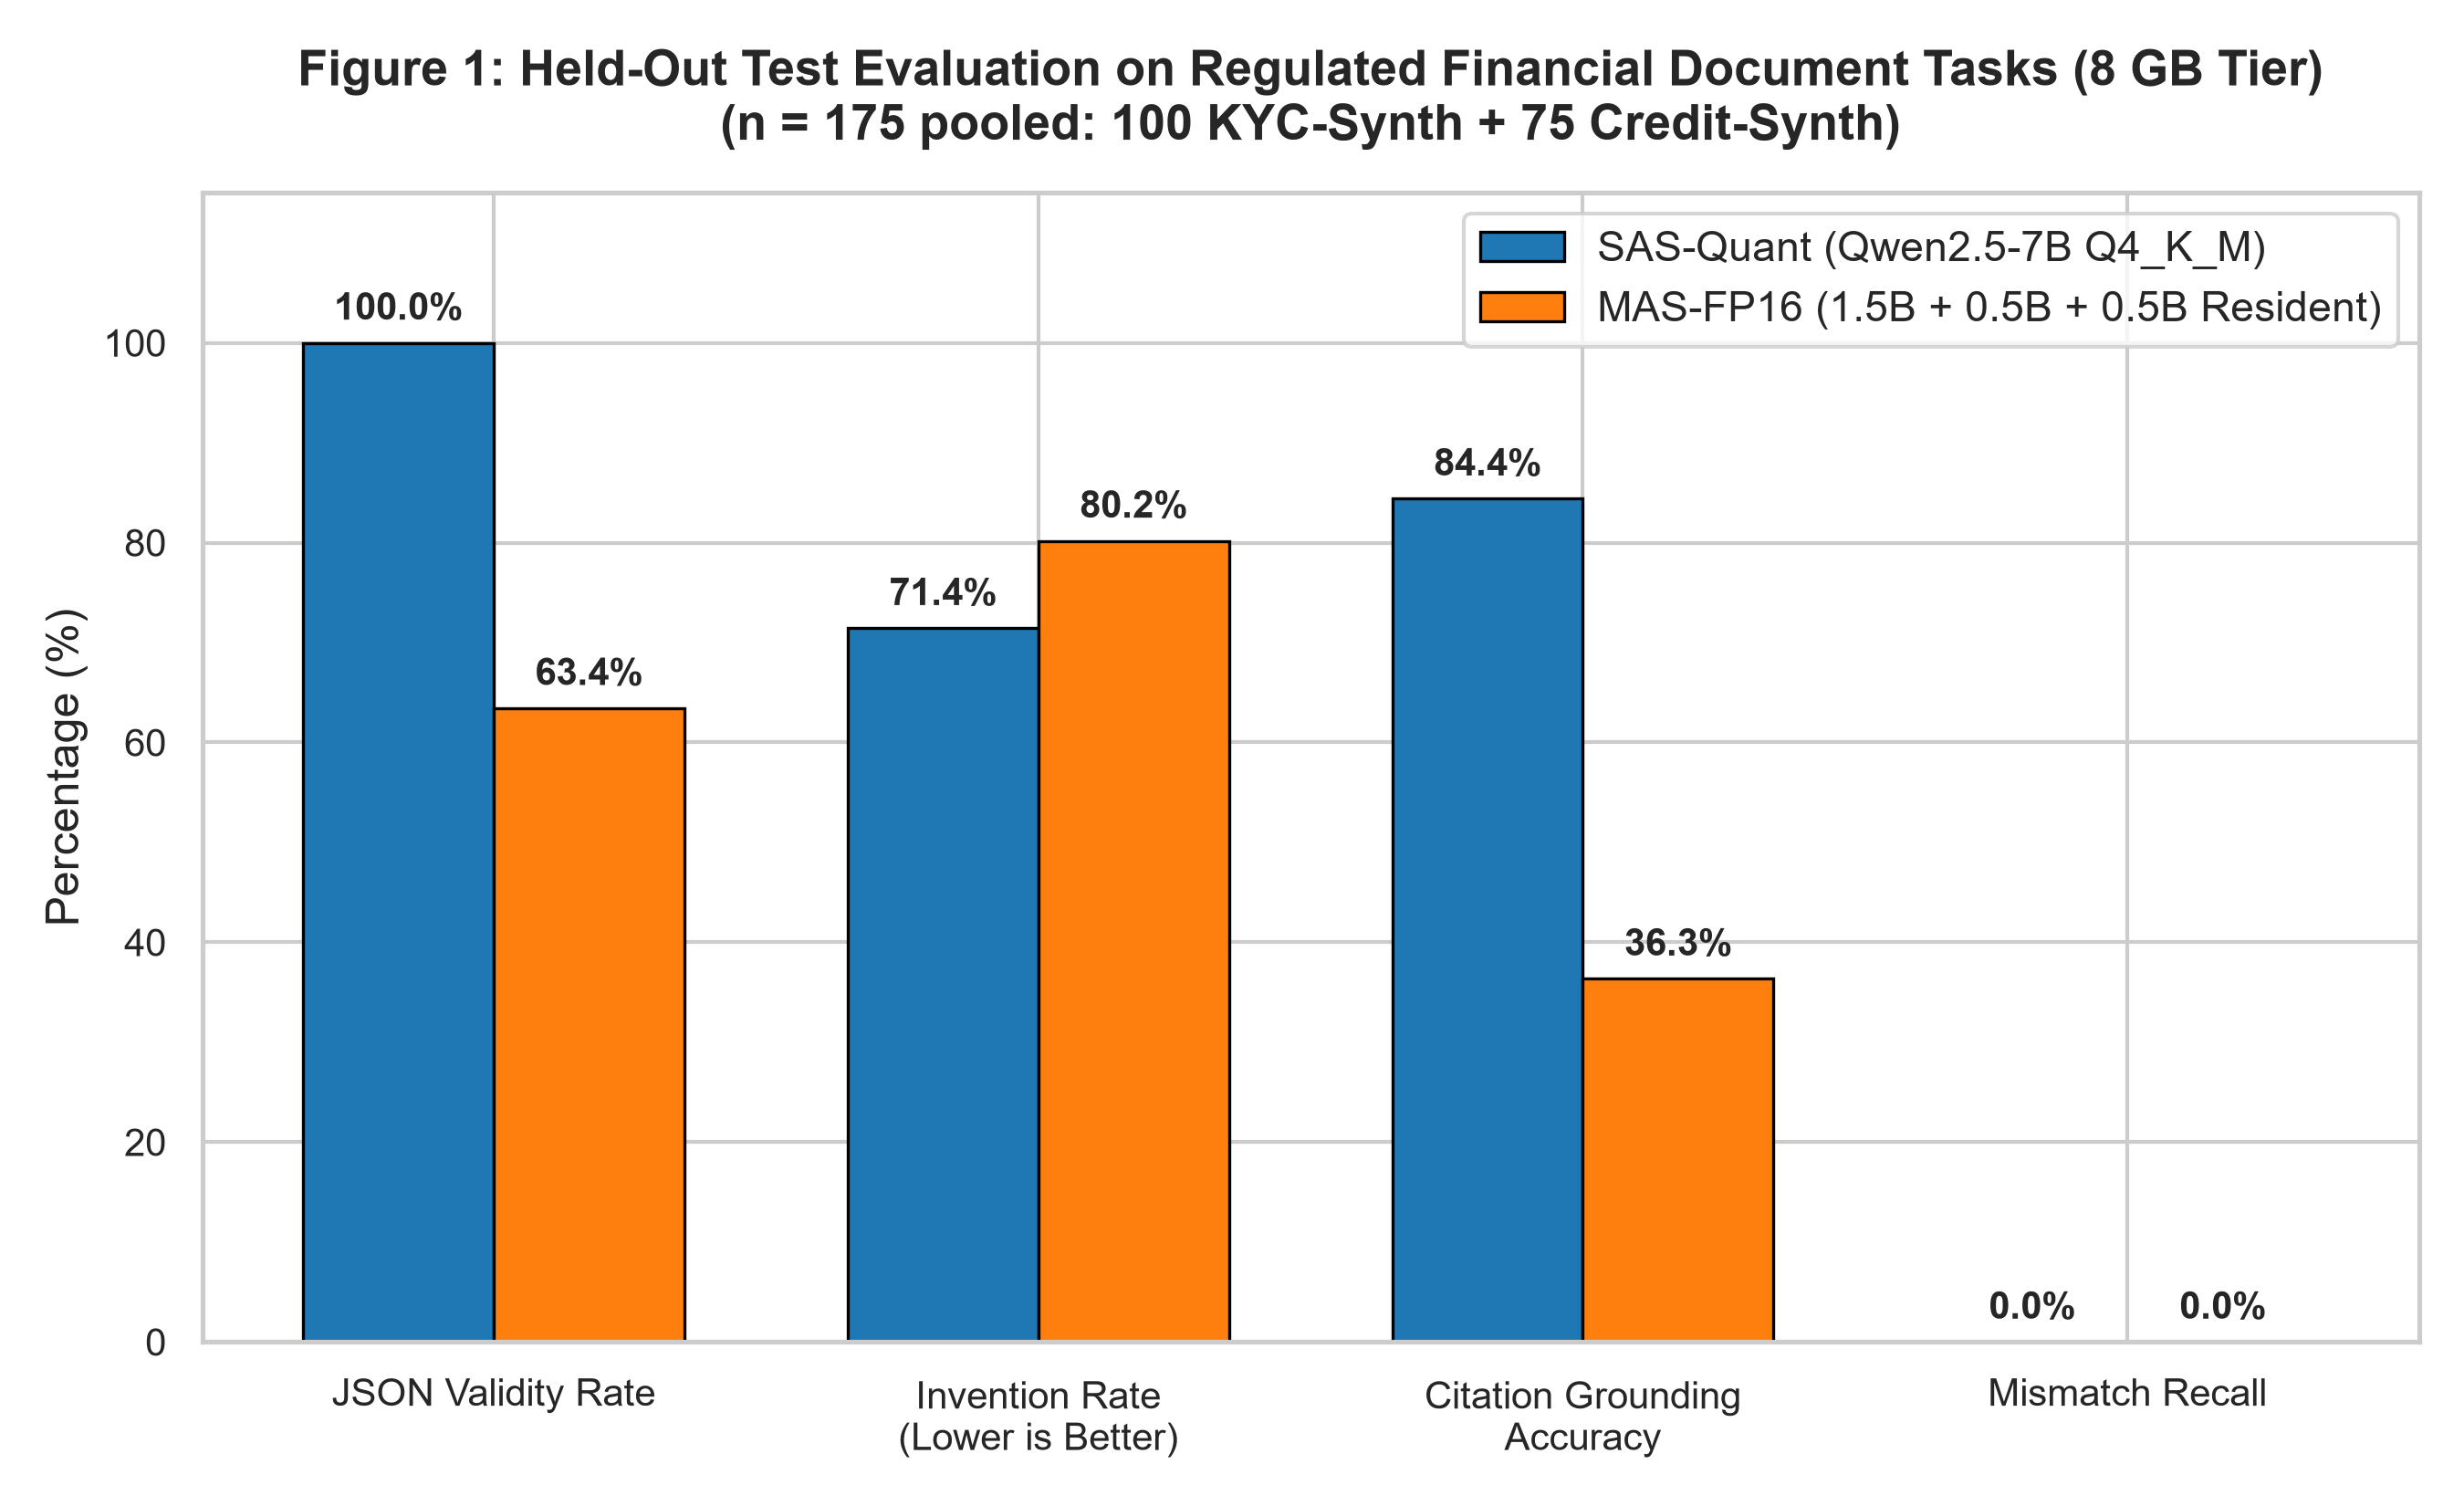
\includegraphics[width=\textwidth,height=0.43\textheight,keepaspectratio]{figures/tier8/figure1_headline_metrics.png}
\caption{Historical 8 GB synthetic headline metrics.}
\label{fig:source-1}
\end{figure*}

\subsection{Redeveloped 8 GB FinQA programme (15 configurations)}\label{redeveloped-8-gb-finqa-programme-15-configurations}

\begin{table*}[tbp]
\centering
\setlength{\tabcolsep}{3pt}
\begin{tabular}{@{}>{\raggedright\arraybackslash}p{199.11pt}>{\raggedright\arraybackslash}p{32.86pt}>{\raggedright\arraybackslash}p{80.49pt}>{\raggedright\arraybackslash}p{83.77pt}>{\raggedright\arraybackslash}p{83.77pt}@{}}
\toprule
\textbf{8 GB condition (reported metric)} & \textbf{N} & \textbf{C / W / H} & \textbf{Raw C / W / H} & \textbf{Peak RSS (GB)} \\
\midrule
Reserved: control SAS & 49 & 8 / 20 / 21 & 14 / 14 / 21 & 5.368 \\
Reserved: control MAS & 49 & 4 / 17 / 28 & 8 / 13 / 28 & 5.052 \\
Reserved: crossed SAS & 49 & 9 / 20 / 20 & 15 / 14 / 20 & 5.364 \\
Reserved: crossed MAS & 49 & 4 / 9 / 36 & 7 / 6 / 36 & 5.064 \\
Selection: baseline SAS & 52 & 8 / 25 / 19 & 10 / 23 / 19 & 5.348 \\
Selection: baseline SAS (analysis128 + 2 demos) & 52 & 9 / 24 / 19 & 10 / 23 / 19 & 5.368 \\
Selection: control SAS & 52 & 8 / 23 / 21 & 10 / 21 / 21 & 5.356 \\
Selection: control SAS (analysis128 + 2 demos) & 52 & 9 / 20 / 23 & 11 / 18 / 23 & 5.365 \\
Selection: crossed SAS & 52 & 10 / 16 / 26 & 12 / 14 / 26 & 5.368 \\
Selection: crossed SAS (analysis128 + 2 demos) & 52 & 9 / 10 / 33 & 10 / 9 / 33 & 5.370 \\
\bottomrule
\end{tabular}
\caption{Redeveloped 8 GB FinQA programme (15 configurations) (rows 1-10)}
\end{table*}

\begin{table*}[tbp]
\centering
\setlength{\tabcolsep}{3pt}
\begin{tabular}{@{}>{\raggedright\arraybackslash}p{202.98pt}>{\raggedright\arraybackslash}p{32.81pt}>{\raggedright\arraybackslash}p{76.94pt}>{\raggedright\arraybackslash}p{83.64pt}>{\raggedright\arraybackslash}p{83.64pt}@{}}
\toprule
\textbf{8 GB condition (reported metric)} & \textbf{N} & \textbf{C / W / H} & \textbf{Raw C / W / H} & \textbf{Peak RSS (GB)} \\
\midrule
Selection: baseline MAS & 52 & 2 / 19 / 31 & 3 / 18 / 31 & 5.058 \\
Selection: baseline original classic MAS & 52 & 4 / 18 / 30 & 6 / 16 / 30 & 5.046 \\
Selection: baseline original critic, common actor & 52 & 4 / 22 / 26 & 6 / 20 / 26 & 5.056 \\
Selection: control MAS & 52 & 3 / 19 / 30 & 5 / 17 / 30 & 5.060 \\
Selection: crossed MAS & 52 & 3 / 15 / 34 & 5 / 13 / 34 & 5.067 \\
\bottomrule
\end{tabular}
\caption{Redeveloped 8 GB FinQA programme (15 configurations) (rows 11-15)}
\end{table*}

In every matched SAS/MAS pair, SAS delivered at least as many correct answers. Adapted critics (``crossed'' negative training) mostly shifted wrong deliveries into withholding rather than adding correct deliveries. The crossed critic withheld one previously correct answer relative to the stronger original critic, so it failed the project's predeclared no-correct-loss adoption rule and was not adopted.

The supporting diagnostics follow the same pattern:

\begin{itemize}
\tightlist
\item
  QLoRA adaptation of the 3B actor added 11 correct \emph{candidates} (delivered states moved from 0/0/24 to 10/11/3).
\item
  A trained critic raised C from 3 to 11 while W rose from 0 to 4.
\item
  A shared-backbone serving proof cut sampled RSS from 4.83 to 2.57 GB with identical logits on a small probe.
\item
  MortarBench gave SAS 39 versus MAS 26 exact answers out of 90; a later FRAMES control gave 2 versus 1 out of 100.
\end{itemize}

\begin{figure*}[tbp]
\centering
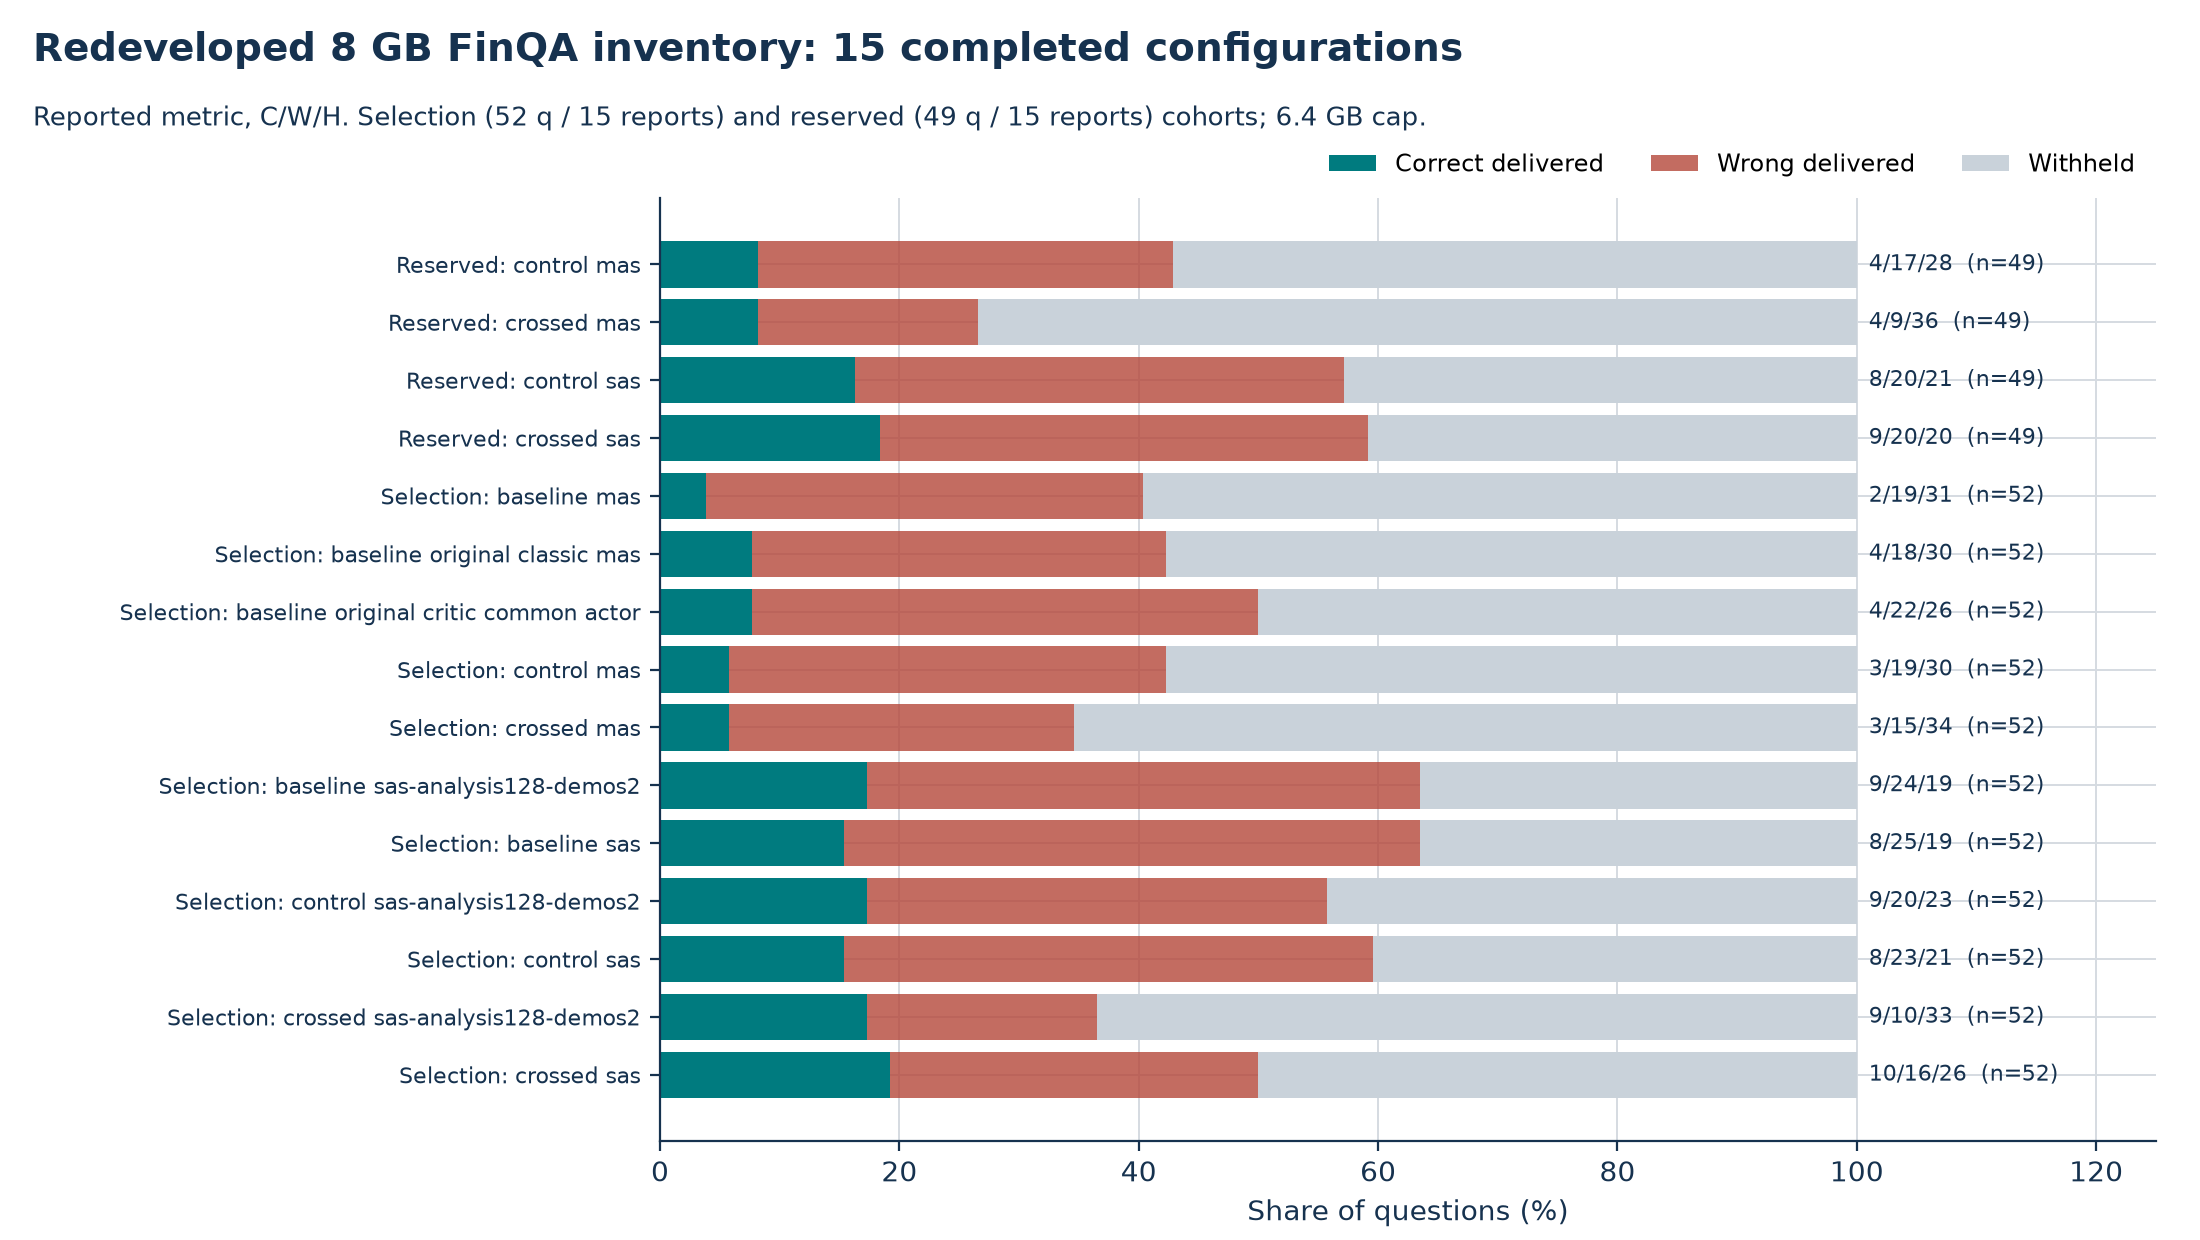
\includegraphics[width=\textwidth,height=0.43\textheight,keepaspectratio]{figures/paper/P08_tier8_inventory.png}
\caption{All 15 completed 8 GB FinQA configurations, reported metric.}
\label{fig:source-2}
\end{figure*}

\subsection{Primary 16 GB results}\label{primary-16-gb-results}

\begin{table*}[tbp]
\centering
\setlength{\tabcolsep}{3pt}
\begin{tabular}{@{}>{\raggedright\arraybackslash}p{130.59pt}>{\raggedright\arraybackslash}p{96.72pt}>{\raggedright\arraybackslash}p{82.20pt}>{\raggedright\arraybackslash}p{88.29pt}>{\raggedright\arraybackslash}p{82.20pt}@{}}
\toprule
\textbf{Profile / arm} & \textbf{Reported C / W / H} & \textbf{Raw C / W / H} & \textbf{Inference hours} & \textbf{Peak RSS (GB)} \\
\midrule
\textbf{Primary / SAS} & \textbf{78 / 48 / 34} & \textbf{38 / 88 / 34} & 11.546 & 10.062 \\
\textbf{Primary / MAS} & \textbf{5 / 3 / 152} & \textbf{5 / 3 / 152} & 2.432 & 10.929 \\
Direct control / SAS & 50 / 66 / 44 & 14 / 102 / 44 & 5.266 & 10.040 \\
Direct control / MAS & 0 / 5 / 155 & 0 / 5 / 155 & 0.821 & 10.901 \\
Repair ablation / SAS & 79 / 50 / 31 & 38 / 91 / 31 & 13.494 & 10.074 \\
Repair ablation / MAS & 5 / 3 / 152 & 5 / 3 / 152 & 3.682 & 10.913 \\
\bottomrule
\end{tabular}
\caption{Primary 16 GB results}
\end{table*}

All six jobs stayed under the 11.5 GB sampled ceiling and completed 160/160 cases. The six jobs used 37.24 inference hours in total.

\textbf{Per-arm rates, primary profile (Wilson 95\%, case-IID, descriptive).}

\begin{table*}[tbp]
\centering
\setlength{\tabcolsep}{3pt}
\begin{tabular}{@{}>{\raggedright\arraybackslash}p{141.01pt}>{\raggedright\arraybackslash}p{117.23pt}>{\raggedright\arraybackslash}p{117.23pt}>{\raggedright\arraybackslash}p{110.53pt}@{}}
\toprule
\textbf{Rate} & \textbf{SAS reported} & \textbf{SAS raw} & \textbf{MAS (both metrics)} \\
\midrule
Correct delivered & 48.8\% [41.1, 56.4] & 23.8\% [17.8, 30.9] & 3.1\% [1.3, 7.1] \\
Wrong delivered & 30.0\% [23.4, 37.5] & 55.0\% [47.3, 62.5] & 1.9\% [0.6, 5.4] \\
Withheld & 21.2\% [15.6, 28.2] & 21.2\% [15.6, 28.2] & 95.0\% [90.4, 97.4] \\
Coverage & 78.8\% & 78.8\% & 5.0\% \\
Precision among delivered & 61.9\% [53.2, 69.9] (78/126) & 30.2\% [22.8, 38.7] (38/126) & 62.5\% [30.6, 86.3] (5/8) \\
\bottomrule
\end{tabular}
\caption{Primary 16 GB results}
\end{table*}

\begin{figure*}[tbp]
\centering
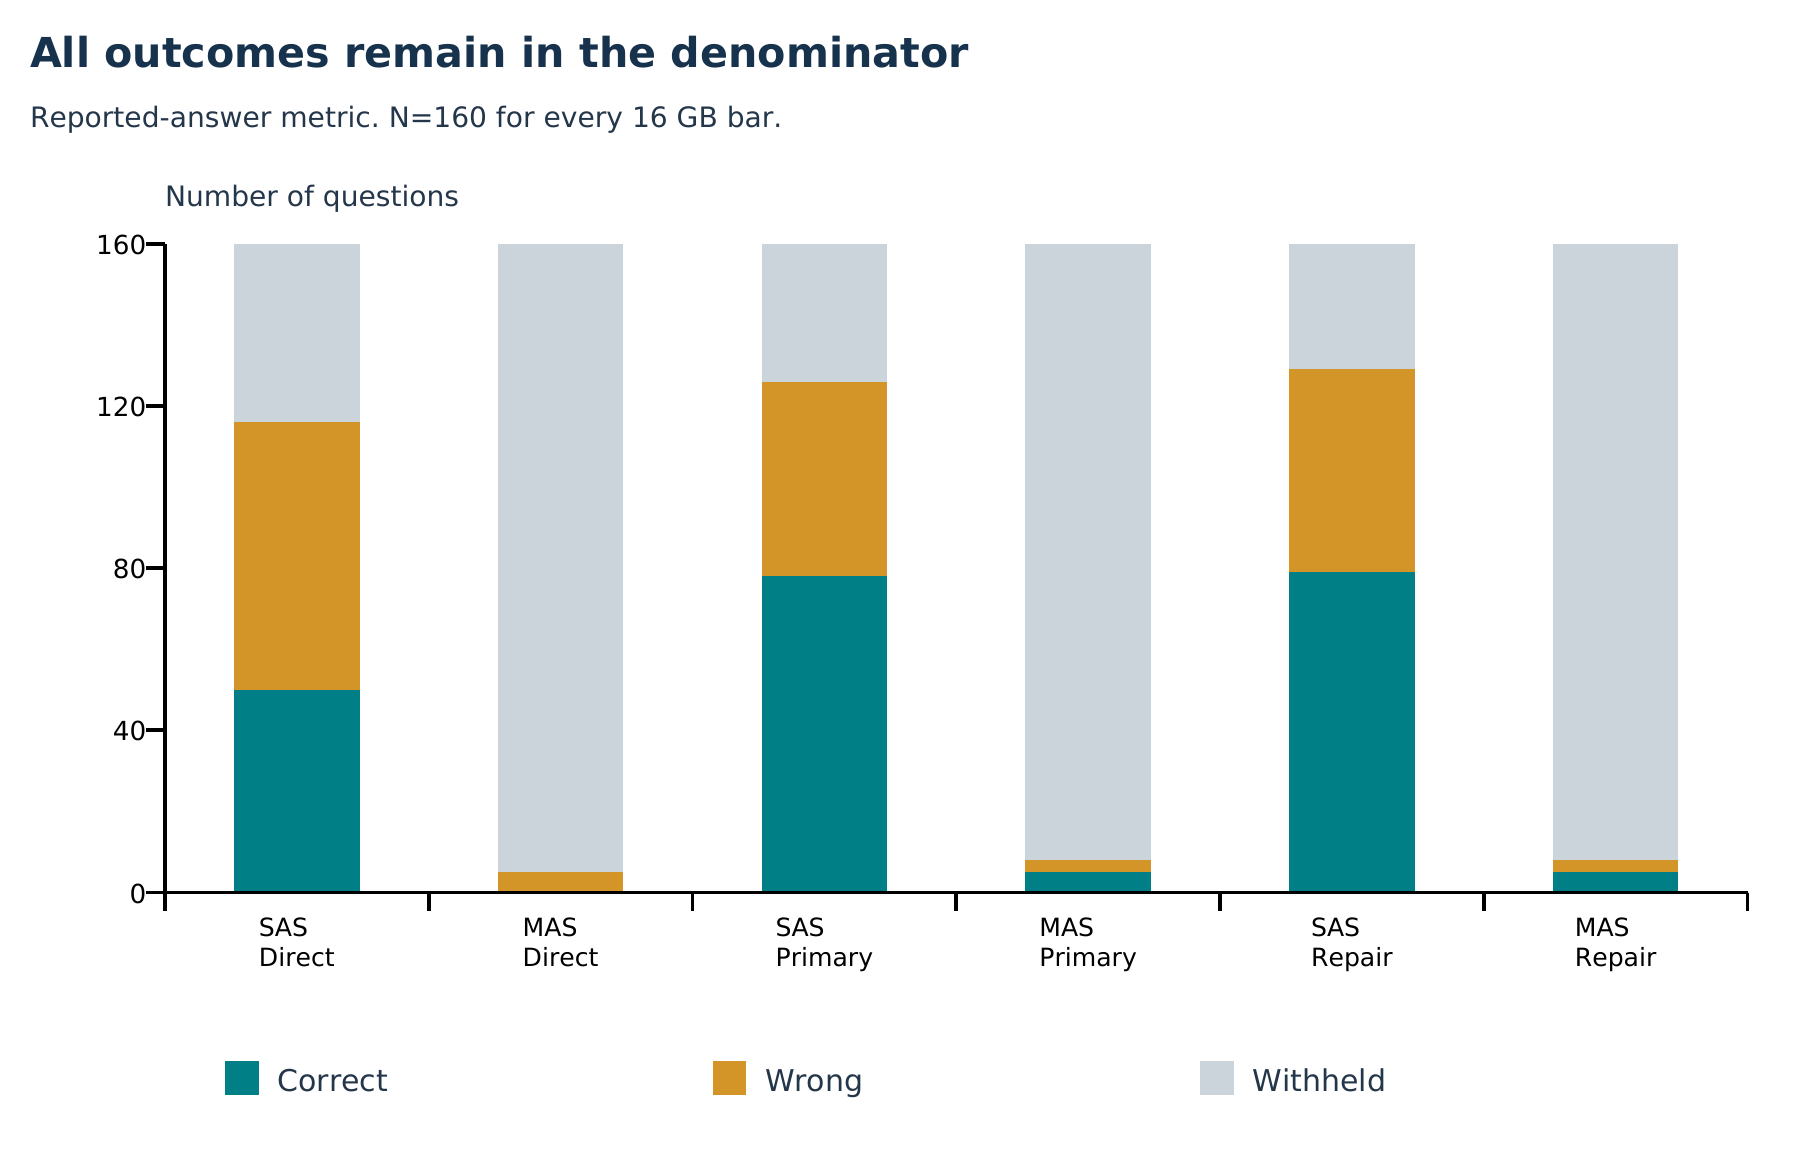
\includegraphics[width=\textwidth,height=0.43\textheight,keepaspectratio]{figures/tier16_v2/01_outcome_profiles.png}
\caption{All six 16 GB jobs: correct, wrong and withheld (reported metric).}
\label{fig:source-3}
\end{figure*}

\subsection{Paired transitions}\label{paired-transitions}

Because both arms answered the same questions, the 3×3 cross-tabulation shows exactly where they differ:

\begin{table*}[tbp]
\centering
\setlength{\tabcolsep}{3pt}
\begin{tabular}{@{}>{\raggedright\arraybackslash}p{234.41pt}>{\raggedright\arraybackslash}p{83.86pt}>{\raggedright\arraybackslash}p{83.86pt}>{\raggedright\arraybackslash}p{83.86pt}@{}}
\toprule
\textbf{SAS state ↓ / MAS state →} & \textbf{MAS C} & \textbf{MAS W} & \textbf{MAS H} \\
\midrule
SAS C (78) & 5 & 1 & \textbf{72} \\
SAS W (48) & 0 & 2 & \textbf{46} \\
SAS H (34) & 0 & 0 & 34 \\
\bottomrule
\end{tabular}
\caption{Paired transitions}
\end{table*}

There is \textbf{no question on which MAS delivered a correct answer that SAS did not}. MAS's 45 fewer wrong deliveries come from withholding 46 questions that SAS got wrong. The same withholding also cost 72 questions that SAS got right. At report level, SAS had a higher correct-delivery rate on 33 of 50 reports, the two tied on 17, and MAS was higher on none.

\begin{figure*}[tbp]
\centering
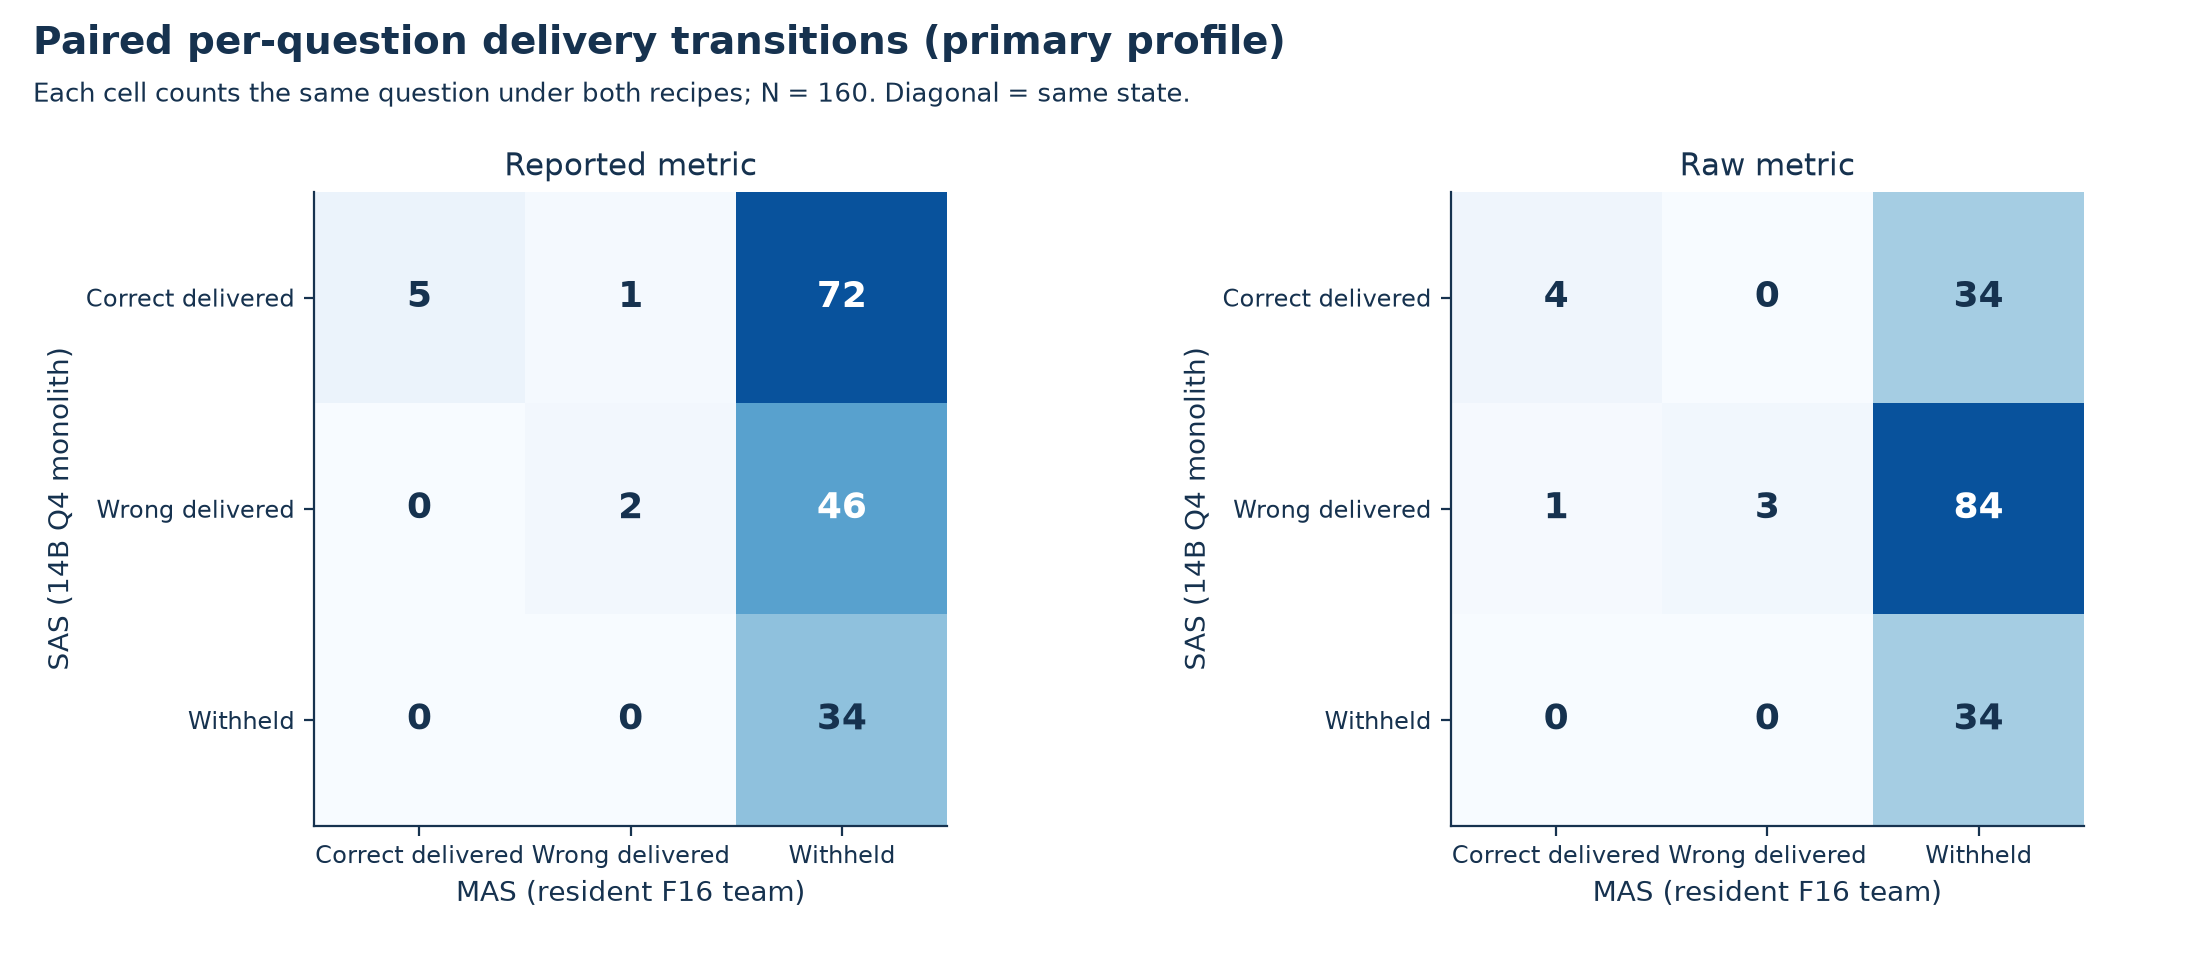
\includegraphics[width=\textwidth,height=0.43\textheight,keepaspectratio]{figures/paper/P01_paired_transitions.png}
\caption{Paired per-question transitions, both metrics.}
\label{fig:source-4}
\end{figure*}

\begin{figure*}[tbp]
\centering
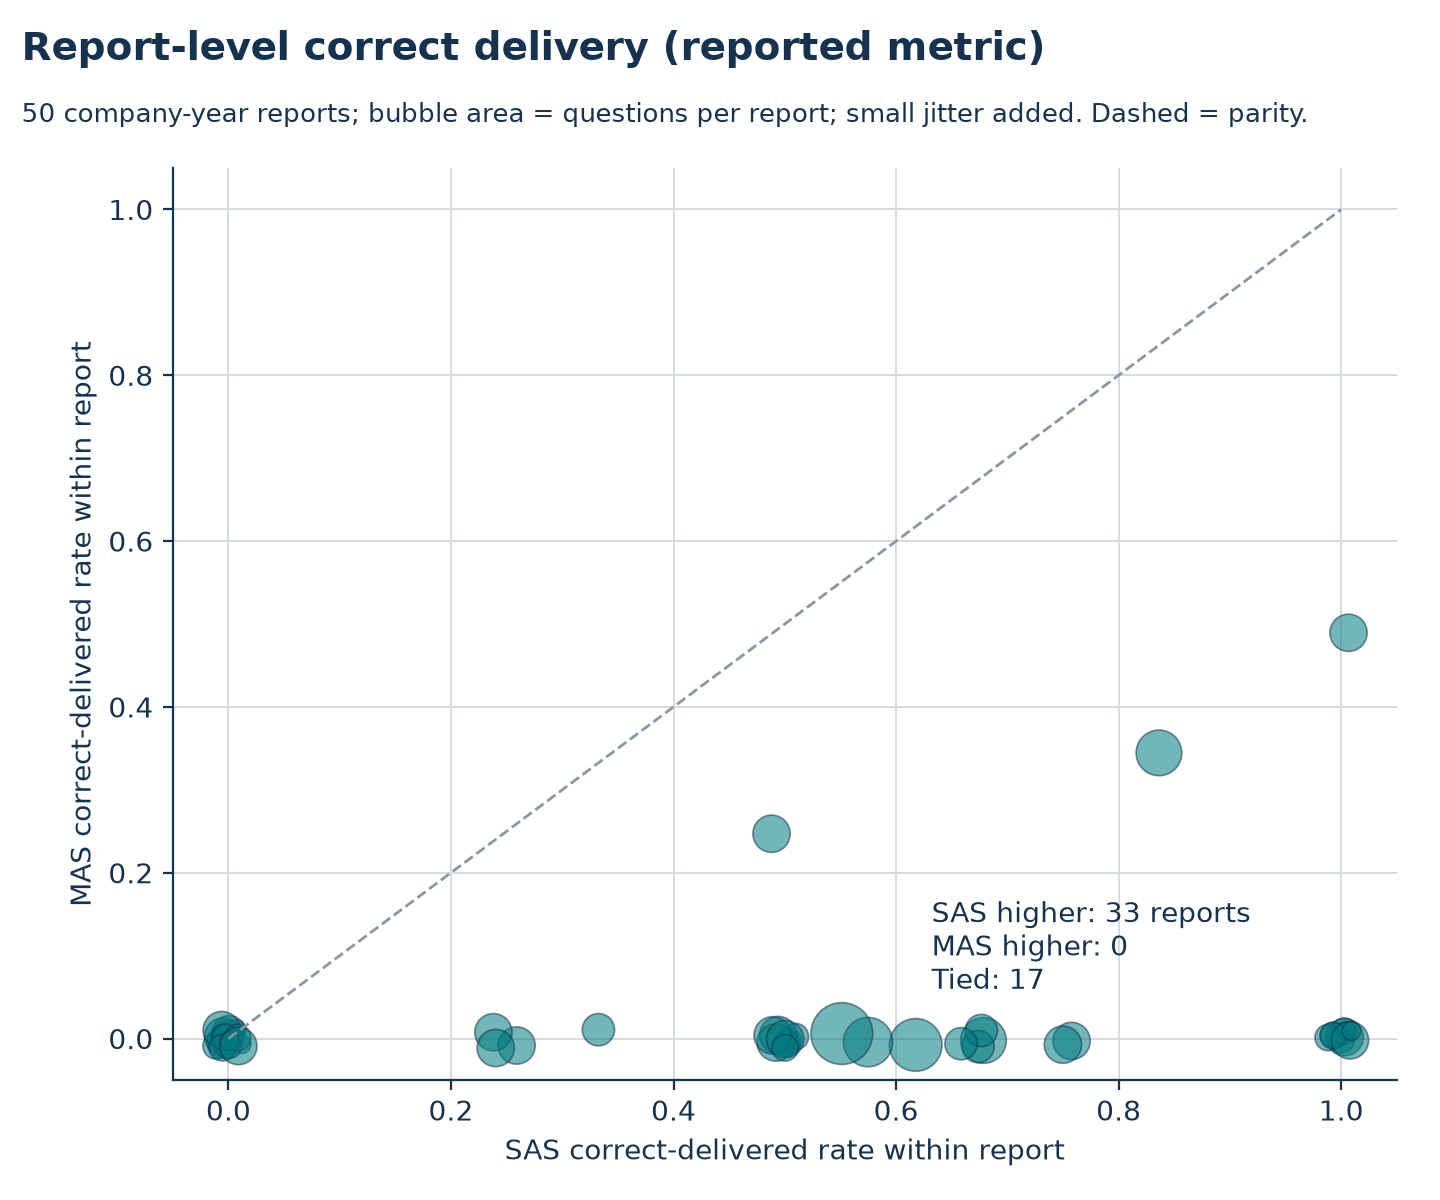
\includegraphics[width=\textwidth,height=0.43\textheight,keepaspectratio]{figures/paper/P03_report_scatter.png}
\caption{Report-level correct-delivery rates; MAS is above parity on no report.}
\label{fig:source-5}
\end{figure*}

\subsection{Statistical inference for the primary contrasts}\label{statistical-inference-for-the-primary-contrasts}

\begin{table*}[tbp]
\centering
\setlength{\tabcolsep}{3pt}
\begin{tabular}{@{}>{\raggedright\arraybackslash}p{133.90pt}>{\raggedright\arraybackslash}p{58.67pt}>{\raggedright\arraybackslash}p{95.81pt}>{\raggedright\arraybackslash}p{95.81pt}>{\raggedright\arraybackslash}p{95.81pt}@{}}
\toprule
\textbf{Endpoint (MAS − SAS)} & \textbf{Δ (pp)} & \textbf{Report 95\% CI} & \textbf{98.75\% CI} & \textbf{Company 95\% CI} \\
\midrule
Reported / correct & −45.62 & [−53.90, −36.55] & [−56.25, −34.09] & [−53.47, −36.44] \\
Reported / wrong & −28.12 & [−37.09, −20.13] & [−39.34, −18.08] & [−38.36, −19.76] \\
Raw / correct & −20.62 & [−28.26, −13.37] & [−30.29, −11.76] & [−28.15, −14.07] \\
Raw / wrong & −53.12 & [−61.90, −44.08] & [−64.49, −41.26] & [−61.99, −43.08] \\
Withheld (identity) & +73.75 & [+64.71, +81.93] & [+62.09, +84.38] & [+66.03, +81.10] \\
\bottomrule
\end{tabular}
\caption{Statistical inference for the primary contrasts (column panel 1 of 2)}
\end{table*}

\begin{table*}[tbp]
\centering
\setlength{\tabcolsep}{3pt}
\begin{tabular}{@{}>{\raggedright\arraybackslash}p{118.96pt}>{\raggedright\arraybackslash}p{102.06pt}>{\raggedright\arraybackslash}p{108.51pt}>{\raggedright\arraybackslash}p{60.19pt}>{\raggedright\arraybackslash}p{90.28pt}@{}}
\toprule
\textbf{Endpoint (MAS − SAS)} & \textbf{Equal-report Δ [95\%]} & \textbf{Leave-one-report-out range} & \textbf{Holm p} & \textbf{McNemar (IID only)} \\
\midrule
Reported / correct & −42.48 [−52.66, −32.31] & [−46.79, −44.23] & 6.1×10⁻⁵ & 2.1×10⁻²² \\
Reported / wrong & −30.62 [−40.75, −20.71] & [−29.53, −26.75] & 6.1×10⁻⁵ & 6.8×10⁻¹³ \\
Raw / correct & −18.74 [−26.17, −11.83] & [−22.15, −19.08] & 6.1×10⁻⁵ & 2.1×10⁻⁹ \\
Raw / wrong & −54.37 [−64.00, −44.50] & [−54.61, −51.92] & 6.1×10⁻⁵ & 5.2×10⁻²⁶ \\
Withheld (identity) & +73.11 [+63.11, +82.27] & [+72.55, +75.64] & — & — \\
\bottomrule
\end{tabular}
\caption{Statistical inference for the primary contrasts (column panel 2 of 2)}
\end{table*}

All four primary contrasts exclude zero under every grouping and weighting. Three of the four sign-flip p-values sit at the Monte Carlo resolution floor of 1/65,537 ≈ 1.5×10⁻⁵ (no extreme draw). For raw-metric correct delivery one of 65,536 draws was as extreme, giving 2/65,537 ≈ 3.1×10⁻⁵; Holm adjustment over the four gives 6.1×10⁻⁵ for all four. We independently re-ran the report-cluster bootstrap from the case-level table, and the published intervals were reproduced to the stated precision. \textbf{Direction matters for interpretation.} The correct-delivery contrasts favour SAS. The wrong-delivery contrasts favour MAS, but only because MAS withholds almost everything. A small p-value does not resolve that trade-off; Section 6.12 frames it as a preference. Section 6.13 reports the complete battery of paired, cluster-adjusted and 3×3 symmetry tests behind these p-values.

\begin{figure*}[tbp]
\centering
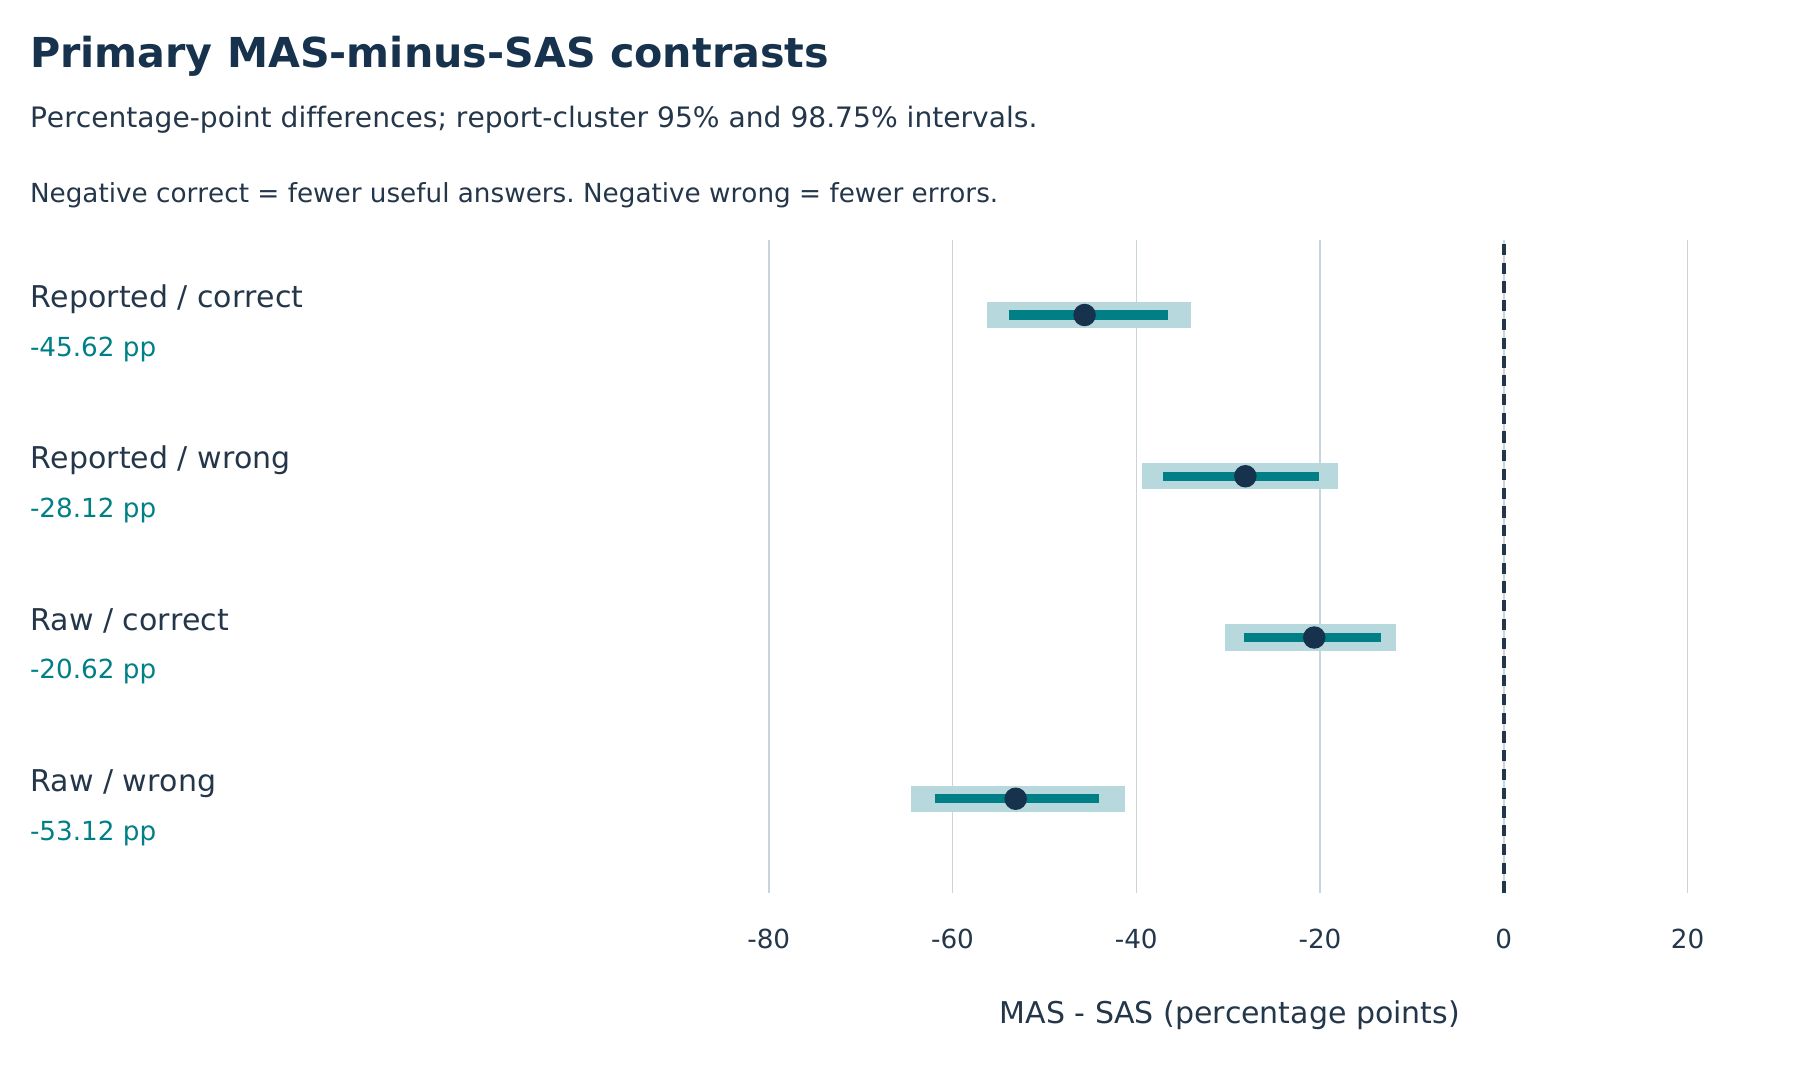
\includegraphics[width=\textwidth,height=0.43\textheight,keepaspectratio]{figures/tier16_v2/02_primary_effects.png}
\caption{Primary effects with report-cluster 95\% and 98.75\% intervals.}
\label{fig:source-6}
\end{figure*}

\begin{figure*}[tbp]
\centering
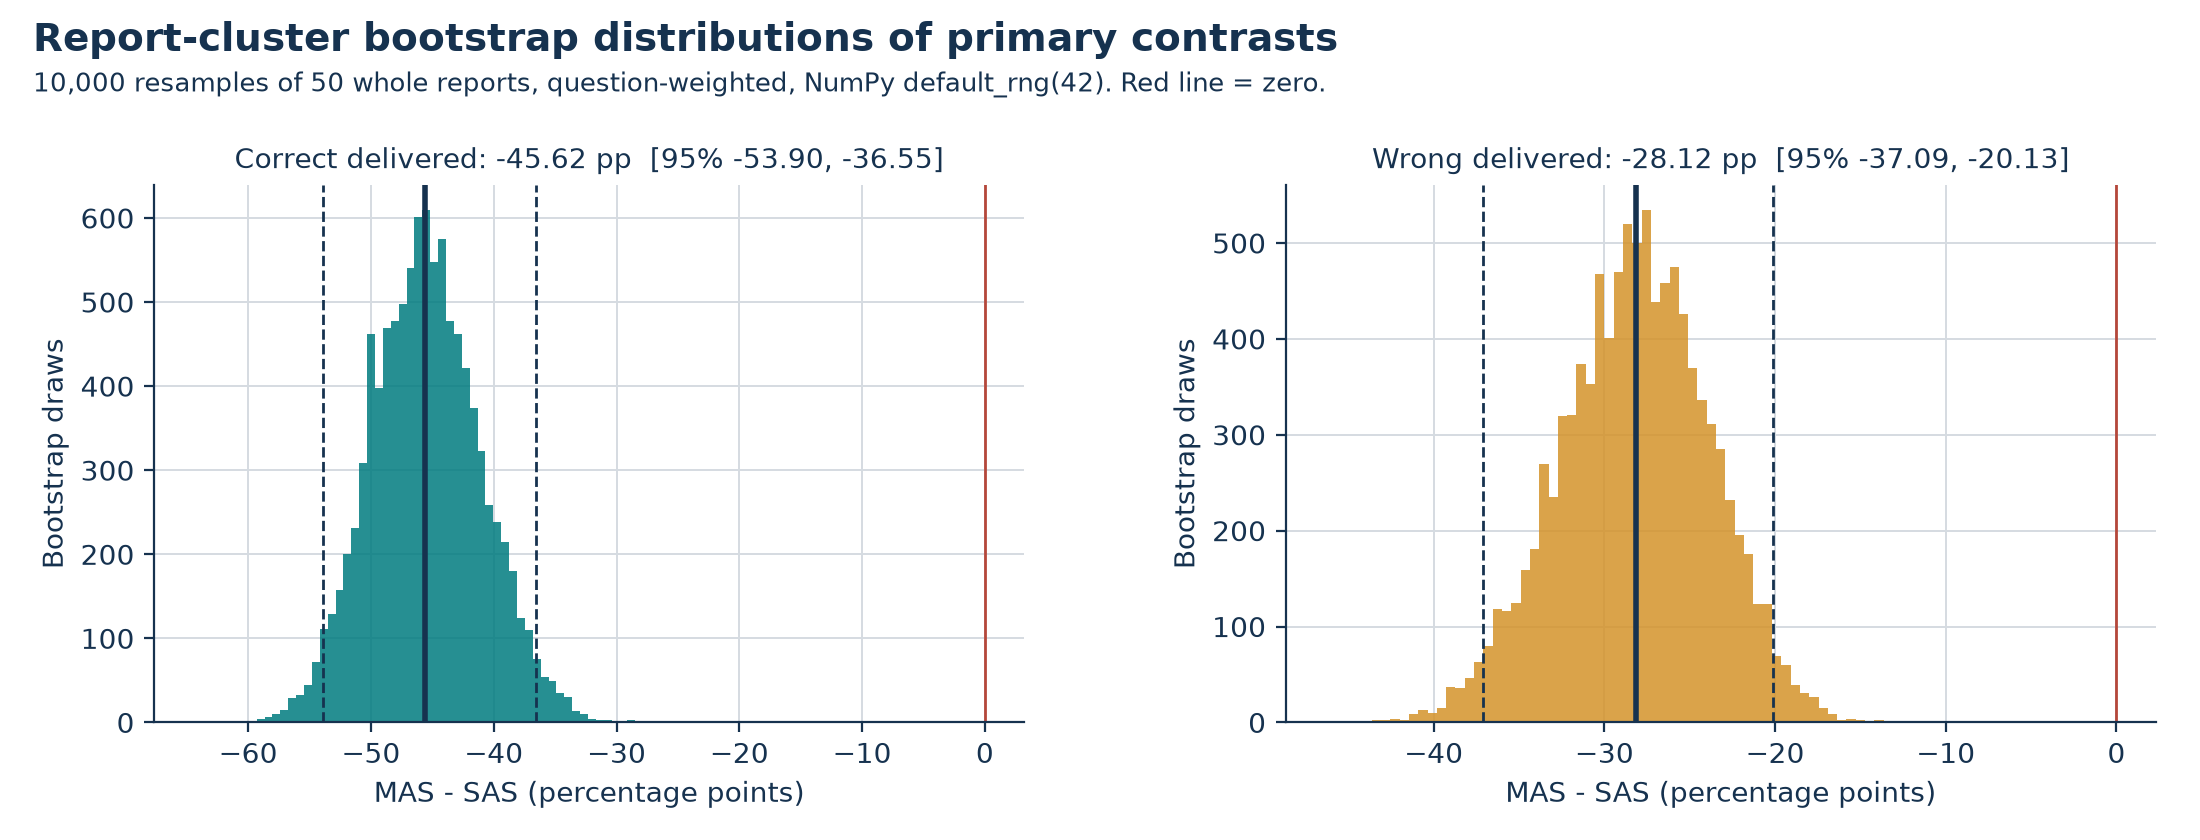
\includegraphics[width=\textwidth,height=0.43\textheight,keepaspectratio]{figures/paper/P02_bootstrap_distributions.png}
\caption{Bootstrap distributions for the reported-metric primary contrasts.}
\label{fig:source-7}
\end{figure*}

\begin{figure*}[tbp]
\centering
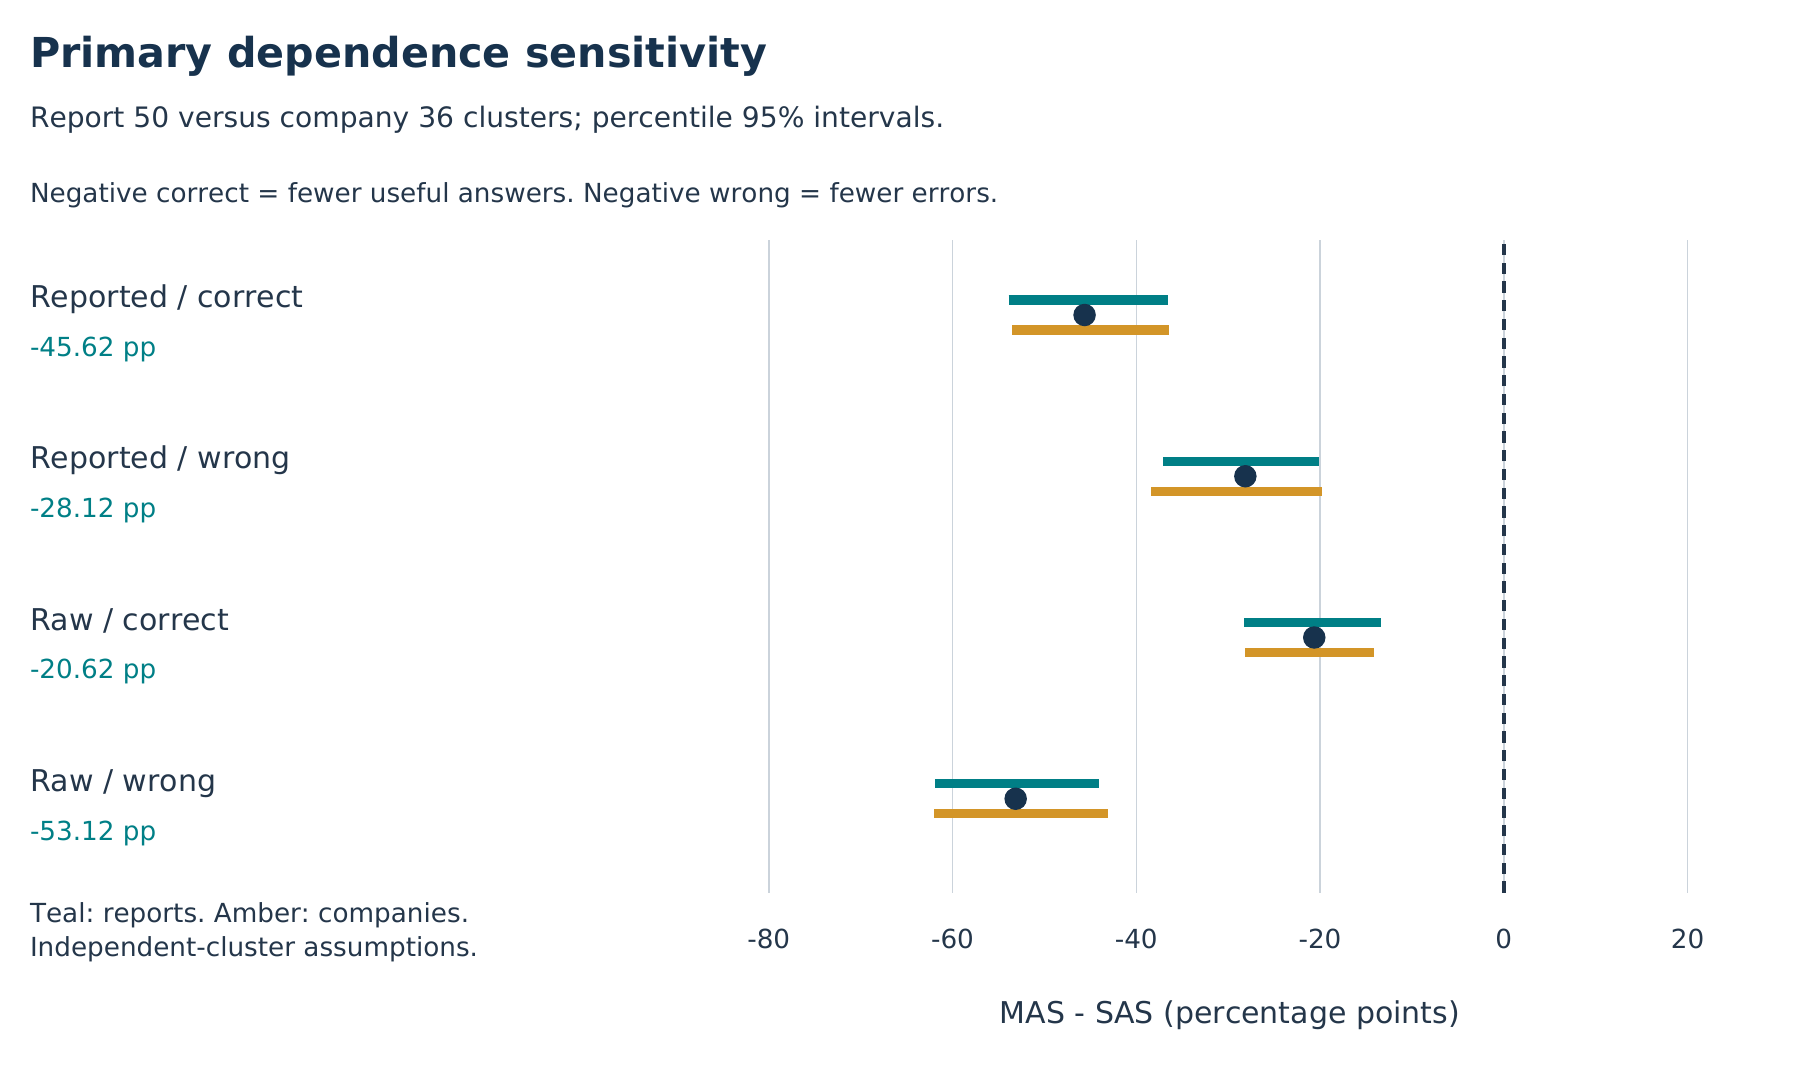
\includegraphics[width=\textwidth,height=0.43\textheight,keepaspectratio]{figures/tier16_v2/11_cluster_sensitivity.png}
\caption{Report- versus company-cluster interval sensitivity.}
\label{fig:source-8}
\end{figure*}

\subsection{Where the team loses useful answers}\label{where-the-team-loses-useful-answers}

\begin{table*}[tbp]
\centering
\setlength{\tabcolsep}{3pt}
\begin{tabular}{@{}>{\raggedright\arraybackslash}p{33.54pt}>{\raggedright\arraybackslash}p{69.27pt}>{\raggedright\arraybackslash}p{63.87pt}>{\raggedright\arraybackslash}p{51.37pt}>{\raggedright\arraybackslash}p{51.37pt}>{\raggedright\arraybackslash}p{61.96pt}>{\raggedright\arraybackslash}p{57.96pt}>{\raggedright\arraybackslash}p{72.65pt}@{}}
\toprule
\textbf{Arm} & \textbf{Executable candidate} & \textbf{Correct candidate} & \textbf{C delivered} & \textbf{W delivered} & \textbf{Correct withheld} & \textbf{Wrong withheld} & \textbf{Invalid / INSUFFICIENT} \\
\midrule
SAS & 150 & 84 & 78 & 48 & 6 & 18 & 10 \\
MAS & 10 & 5 & 5 & 3 & 0 & 2 & 150 \\
\bottomrule
\end{tabular}
\caption{Where the team loses useful answers}
\end{table*}

All 160 program-stage responses were valid JSON in both arms. The grammar solved format; it did not ensure useful content. The 14B model chose ANSWER on 150 questions. The 3B drafter chose INSUFFICIENT on 150. Writing \(q\) for the executable fraction, \(p\) for correctness given execution, and \(a\) and \(b\) for gate acceptance of correct and wrong candidates:

\begin{table*}[tbp]
\centering
\setlength{\tabcolsep}{3pt}
\begin{tabular}{@{}>{\raggedright\arraybackslash}p{56.43pt}>{\raggedright\arraybackslash}p{63.84pt}>{\raggedright\arraybackslash}p{58.28pt}>{\raggedright\arraybackslash}p{58.28pt}>{\raggedright\arraybackslash}p{58.28pt}>{\raggedright\arraybackslash}p{86.44pt}>{\raggedright\arraybackslash}p{86.44pt}@{}}
\toprule
\textbf{} & \textbf{$q$} & \textbf{$p$} & \textbf{$a$} & \textbf{$b$} & \textbf{$C/N=q\,p\,a$} & \textbf{$W/N=q(1-p)b$} \\
\midrule
SAS & 0.9375 & 0.560 & 0.929 & 0.727 & 78/160 & 48/160 \\
MAS & 0.0625 & 0.500 & 1.000 & 0.600 & 5/160 & 3/160 \\
\bottomrule
\end{tabular}
\caption{Where the team loses useful answers}
\end{table*}

The binding factor for MAS is \(q\), a fifteen-fold gap in executable candidate production. The review gates behave similarly: neither is a strong error filter. The 14B reviewer accepted 73\% of wrong executable candidates and the 0.5B verifier 60\%.

\begin{figure*}[tbp]
\centering
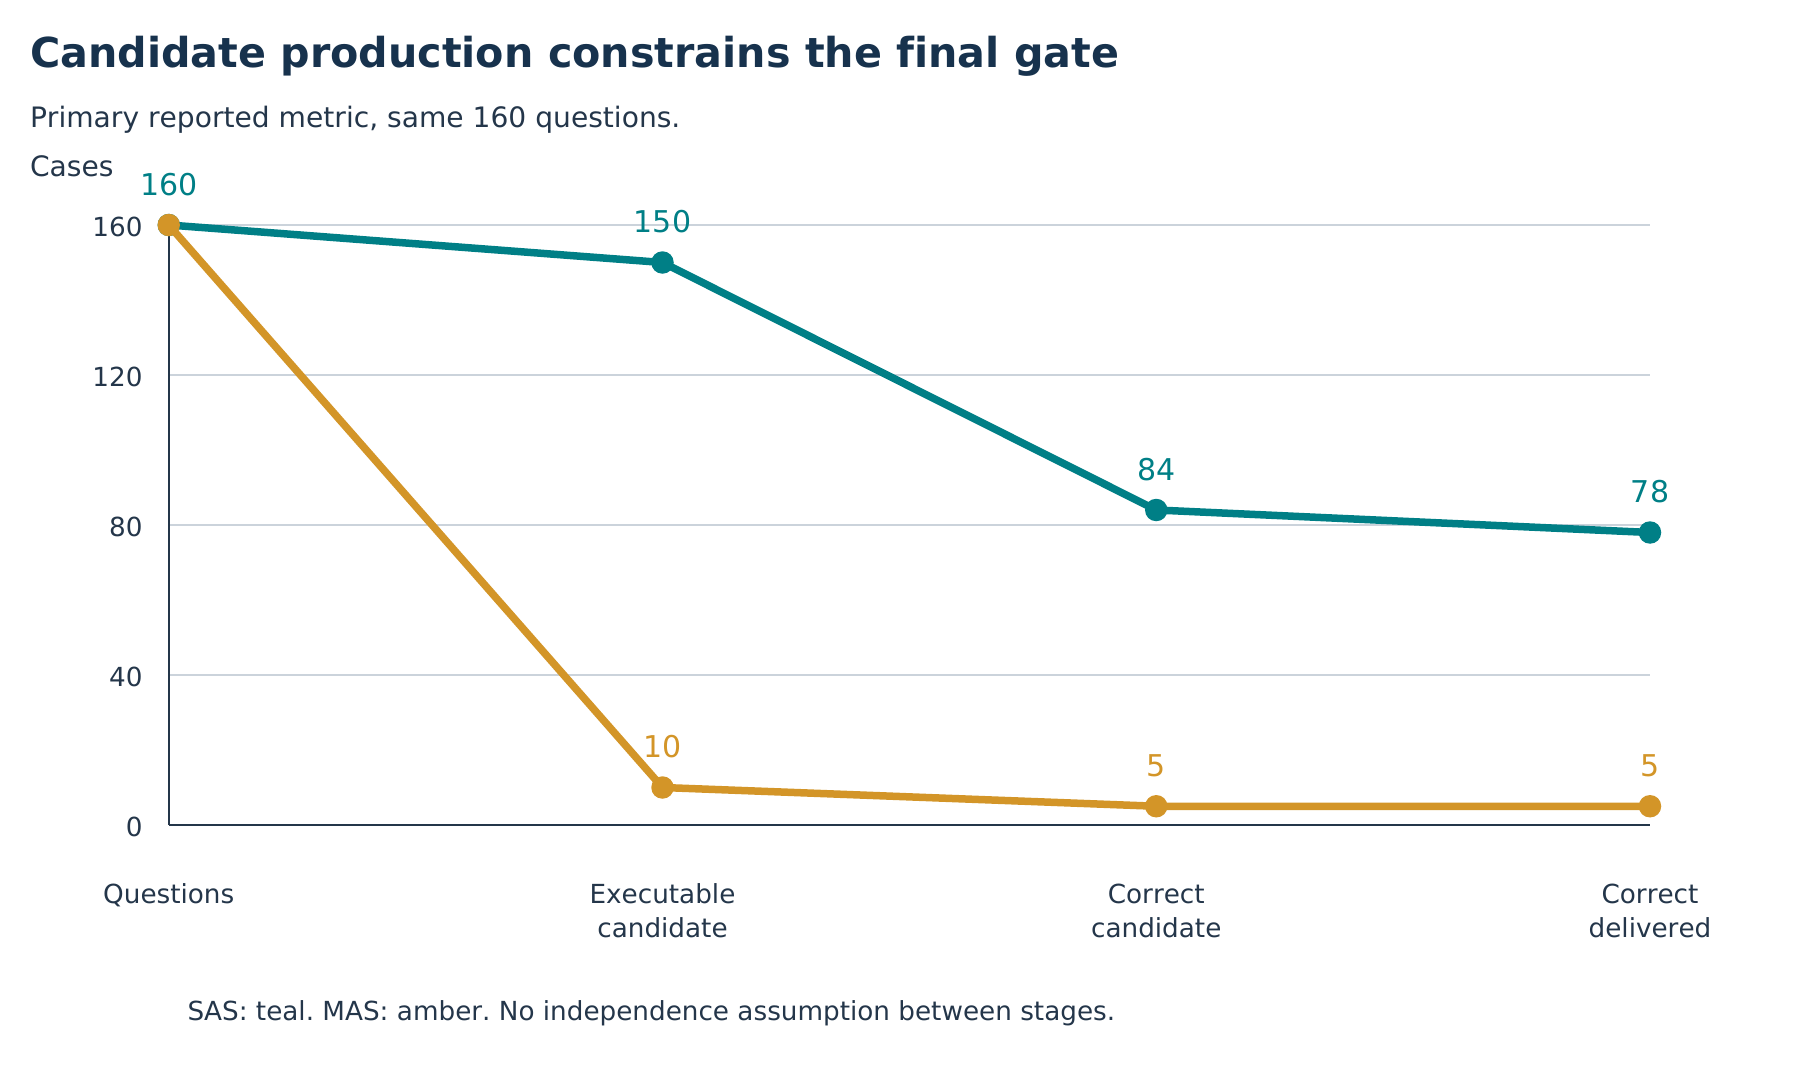
\includegraphics[width=\textwidth,height=0.43\textheight,keepaspectratio]{figures/tier16_v2/03_candidate_funnel.png}
\caption{Candidate production constrains the final gate.}
\label{fig:source-9}
\end{figure*}

\subsection{Prompt bundle and repair ablations}\label{prompt-bundle-and-repair-ablations}

\begin{table*}[tbp]
\centering
\setlength{\tabcolsep}{3pt}
\begin{tabular}{@{}>{\raggedright\arraybackslash}p{141.84pt}>{\raggedright\arraybackslash}p{66.92pt}>{\raggedright\arraybackslash}p{40.98pt}>{\raggedright\arraybackslash}p{40.98pt}>{\raggedright\arraybackslash}p{91.64pt}>{\raggedright\arraybackslash}p{91.64pt}@{}}
\toprule
\textbf{Contrast (right − left)} & \textbf{Metric} & \textbf{ΔC} & \textbf{ΔW} & \textbf{C 95\% CI (pp)} & \textbf{W 95\% CI (pp)} \\
\midrule
SAS primary vs direct & Reported & +28 & −18 & [+9.76, +24.55] & [−17.98, −3.90] \\
SAS primary vs direct & Raw & +24 & −14 & [+8.59, +21.62] & [−17.96, +0.72] \\
MAS primary vs direct & Both & +5 & −2 & [0.00, +6.98] & [−5.26, +2.55] \\
SAS repair vs primary & Reported & +1 & +2 & [0.00, +2.04] & [0.00, +3.40] \\
SAS repair vs primary & Raw & 0 & +3 & [0.00, 0.00] & [0.00, +4.35] \\
MAS repair vs primary & Both & 0 & 0 & [0.00, 0.00] & [0.00, 0.00] \\
\bottomrule
\end{tabular}
\caption{Prompt bundle and repair ablations}
\end{table*}

\textbf{H2 is supported descriptively for both arms}: the analysis-plus-demonstration bundle helped. Direct-control MAS delivered no correct answer at all. The two components cannot be separated with this design. \textbf{H3 is not supported.} Primary and repair runs were identical on all 160 initial decisions in both arms. SAS repair released 3 previously withheld cases (one correct, two wrong under the reported metric; zero correct, three wrong under raw) at a cost of 1.95 extra inference hours. MAS attempted 152 repairs with no change to any delivery state; source-supported candidate programs actually fell from 10 to 8. That cost 1.25 extra hours.

\begin{figure*}[tbp]
\centering
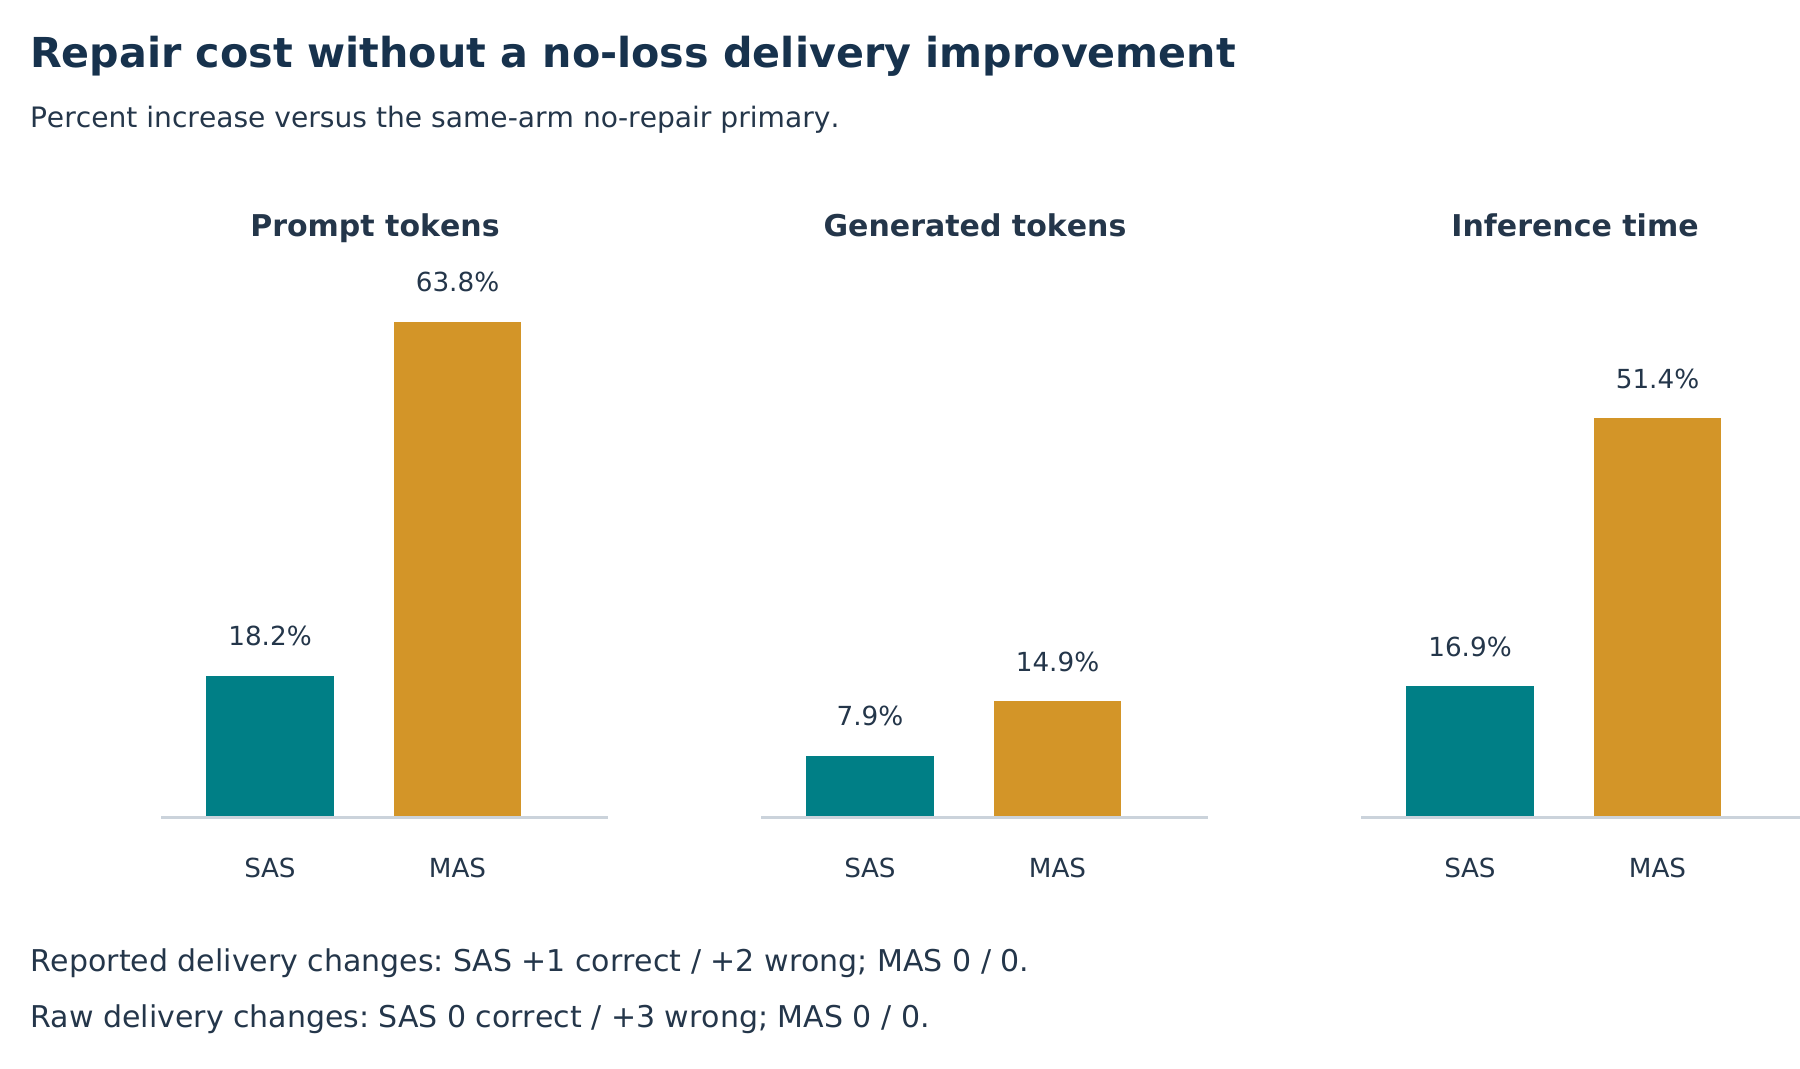
\includegraphics[width=\textwidth,height=0.43\textheight,keepaspectratio]{figures/tier16_v2/06_repair_cost.png}
\caption{Repair cost relative to primary.}
\label{fig:source-10}
\end{figure*}

\subsection{Scoring-convention sensitivity}\label{scoring-convention-sensitivity}

\begin{table*}[tbp]
\centering
\setlength{\tabcolsep}{3pt}
\begin{tabular}{@{}>{\raggedright\arraybackslash}p{189.69pt}>{\raggedright\arraybackslash}p{107.31pt}>{\raggedright\arraybackslash}p{116.65pt}>{\raggedright\arraybackslash}p{72.35pt}@{}}
\toprule
\textbf{SAS primary deliveries} & \textbf{Raw correct} & \textbf{Raw incorrect} & \textbf{Total} \\
\midrule
Reported correct & 34 & 44 & 78 \\
Reported incorrect & 4 & 44 & 48 \\
Total & 38 & 88 & 126 \\
\bottomrule
\end{tabular}
\caption{Scoring-convention sensitivity}
\end{table*}

48 of 126 SAS deliveries change label between conventions. Most are percentage-versus-fraction conventions in the reference data. For example, \path|ABMD/2007/page_52.pdf-2| predicts 59.48 (percent) against reported answer ``59.5\%'' but raw \path|exe_ans| 0.59482. All eight MAS deliveries are concordant. The ordering of arms is the same under both conventions, but SAS's absolute accuracy depends heavily on the convention. That is why both are reported and neither is called ``official''.

\begin{figure*}[tbp]
\centering
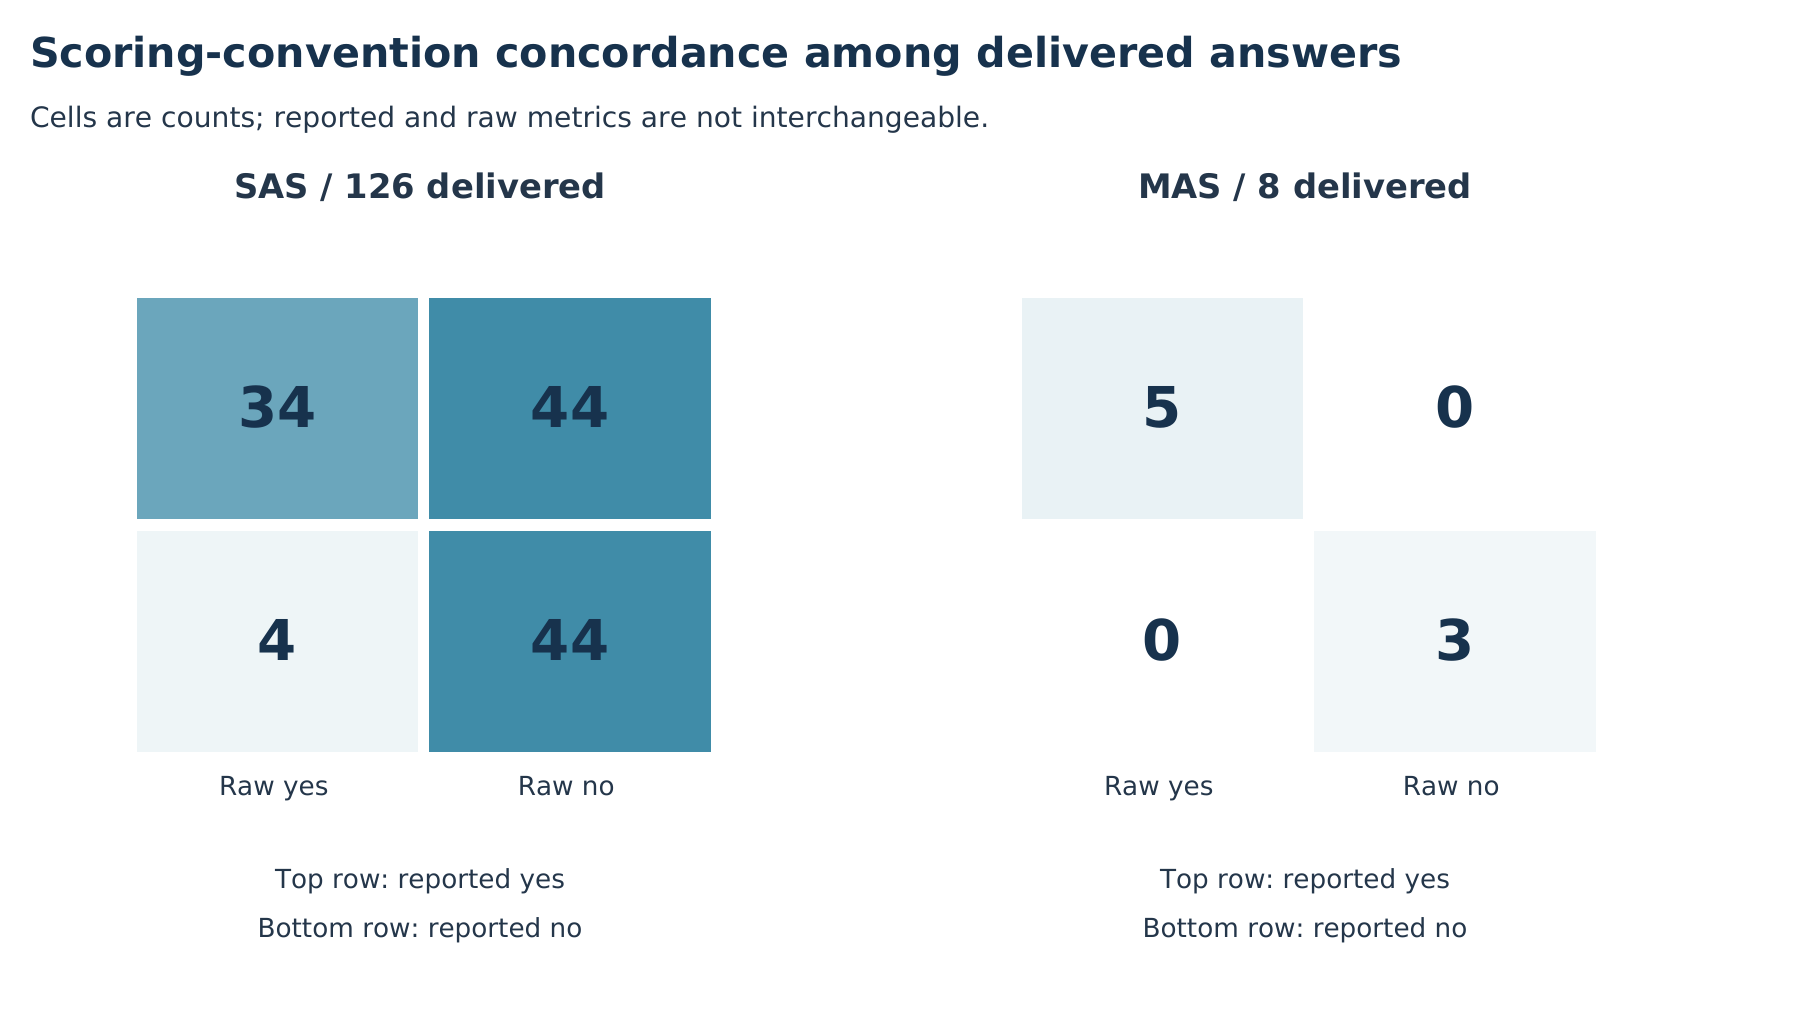
\includegraphics[width=\textwidth,height=0.43\textheight,keepaspectratio]{figures/tier16_v2/04_metric_concordance.png}
\caption{Scoring-convention concordance.}
\label{fig:source-11}
\end{figure*}

\subsection{Post-hoc strata: reasoning complexity and retrieval}\label{post-hoc-strata-reasoning-complexity-and-retrieval}

We stratified by the length and type of the \emph{gold} reference program, which deployment never sees (exploratory):

\begin{table*}[tbp]
\centering
\setlength{\tabcolsep}{3pt}
\begin{tabular}{@{}>{\raggedright\arraybackslash}p{216.44pt}>{\raggedright\arraybackslash}p{52.21pt}>{\raggedright\arraybackslash}p{108.68pt}>{\raggedright\arraybackslash}p{108.68pt}@{}}
\toprule
\textbf{Gold program} & \textbf{n} & \textbf{SAS C / W / H} & \textbf{MAS C / W / H} \\
\midrule
1 step & 104 & 52 / 29 / 23 & 5 / 3 / 96 \\
2 steps & 49 & 26 / 14 / 9 & 0 / 0 / 49 \\
3+ steps & 7 & 0 / 5 / 2 & 0 / 0 / 7 \\
Single add/subtract & 40 & 16 / 12 / 12 & 1 / 0 / 39 \\
Single ratio/product & 59 & 34 / 14 / 11 & 4 / 3 / 52 \\
Multi-step arithmetic & 56 & 26 / 19 / 11 & 0 / 0 / 56 \\
Table aggregate (max/min/sum/avg) & 5 & 2 / 3 / 0 & 0 / 0 / 5 \\
\bottomrule
\end{tabular}
\caption{Post-hoc strata: reasoning complexity and retrieval}
\end{table*}

MAS delivered nothing on any question whose reference solution needs more than one operation. SAS kept about 50\% correct delivery on one- and two-step questions but none on the seven longest programs.

Retrieval completeness tells a similar story. All annotated gold evidence was in the top-8 packet for 138/160 questions. In that stratum SAS delivered 74 correct with only 3 invalid outputs, whereas MAS delivered 5 correct with 128 invalid outputs. The MAS deficit is therefore not explained by missing evidence.

\begin{figure*}[tbp]
\centering
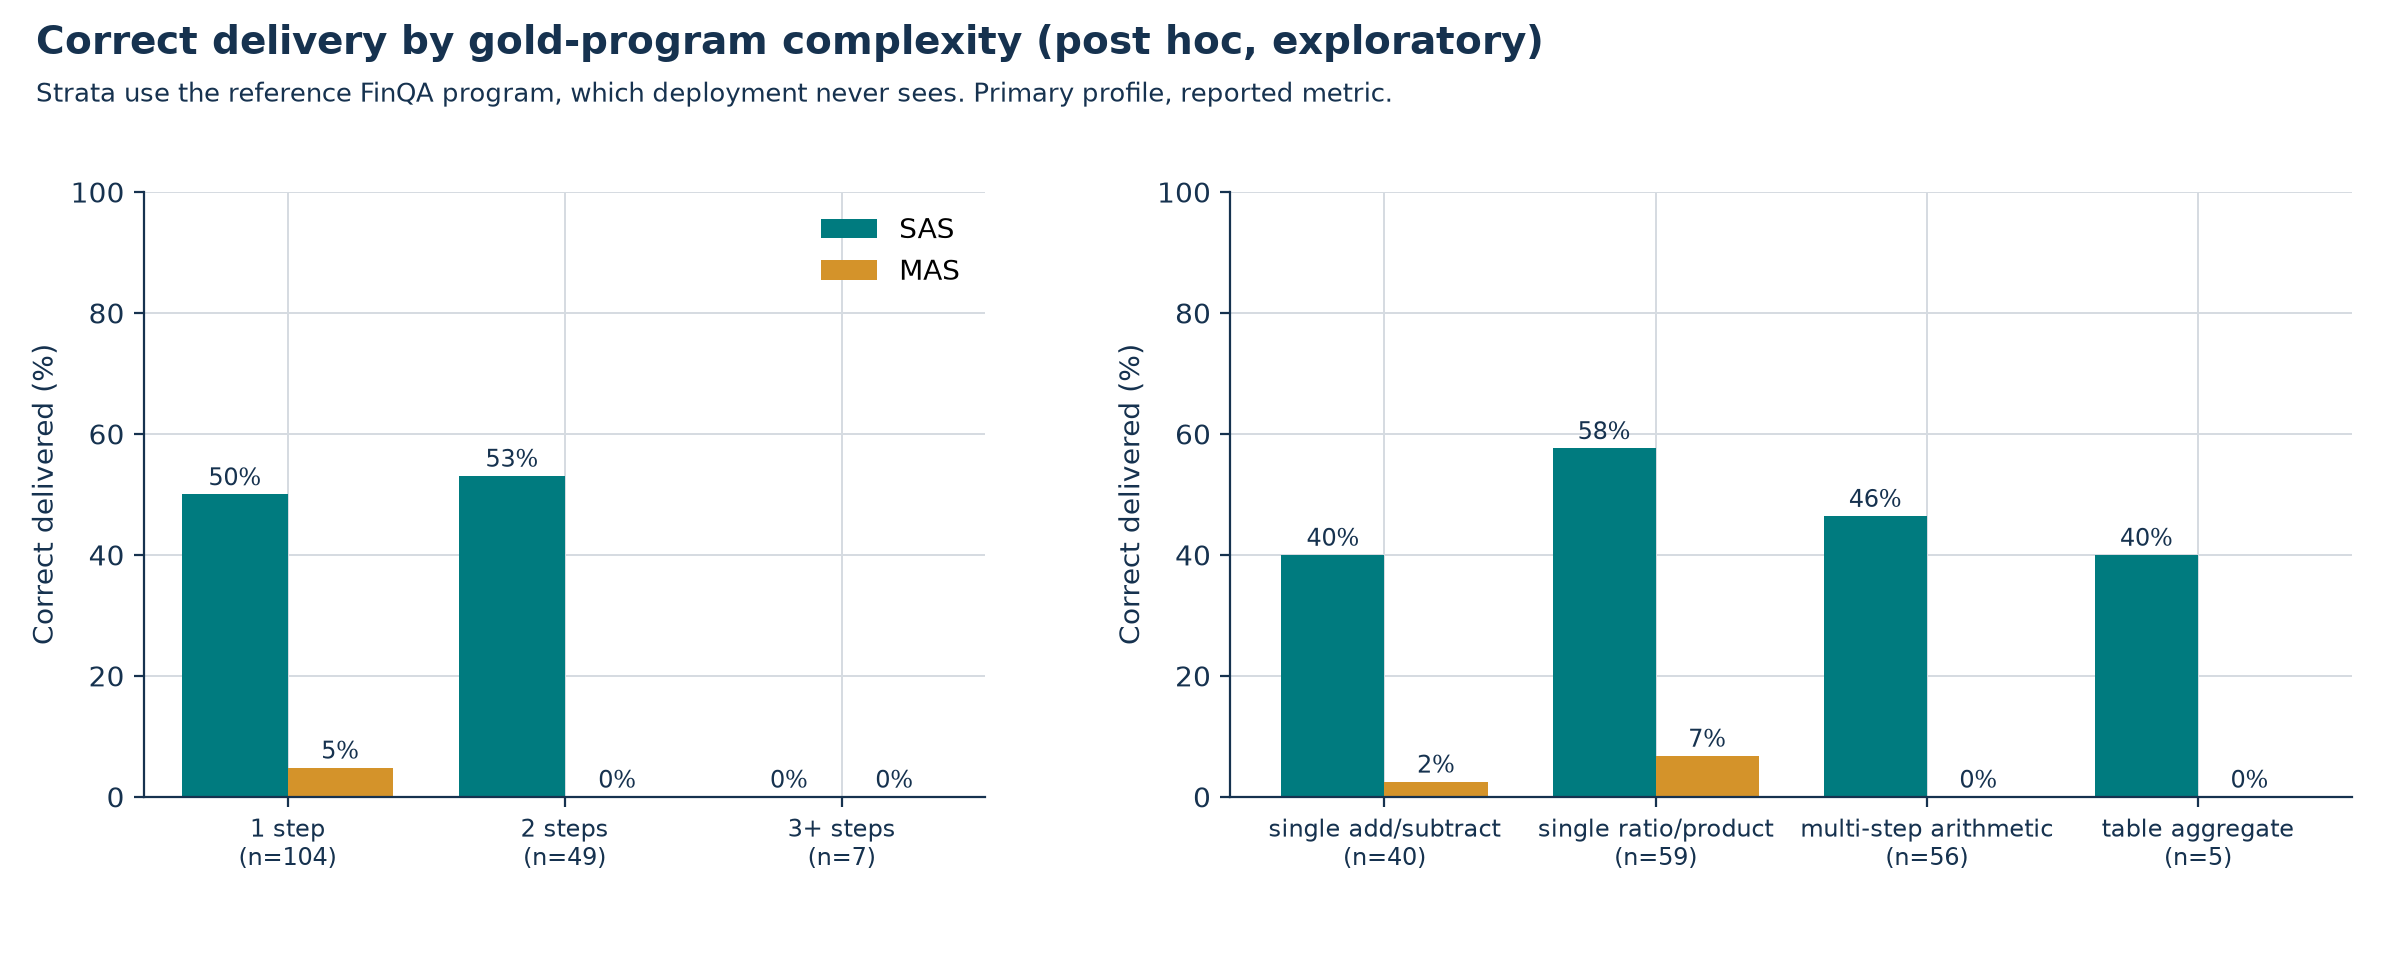
\includegraphics[width=\textwidth,height=0.43\textheight,keepaspectratio]{figures/paper/P04_program_complexity.png}
\caption{Correct delivery by gold-program complexity.}
\label{fig:source-12}
\end{figure*}

\begin{figure*}[tbp]
\centering
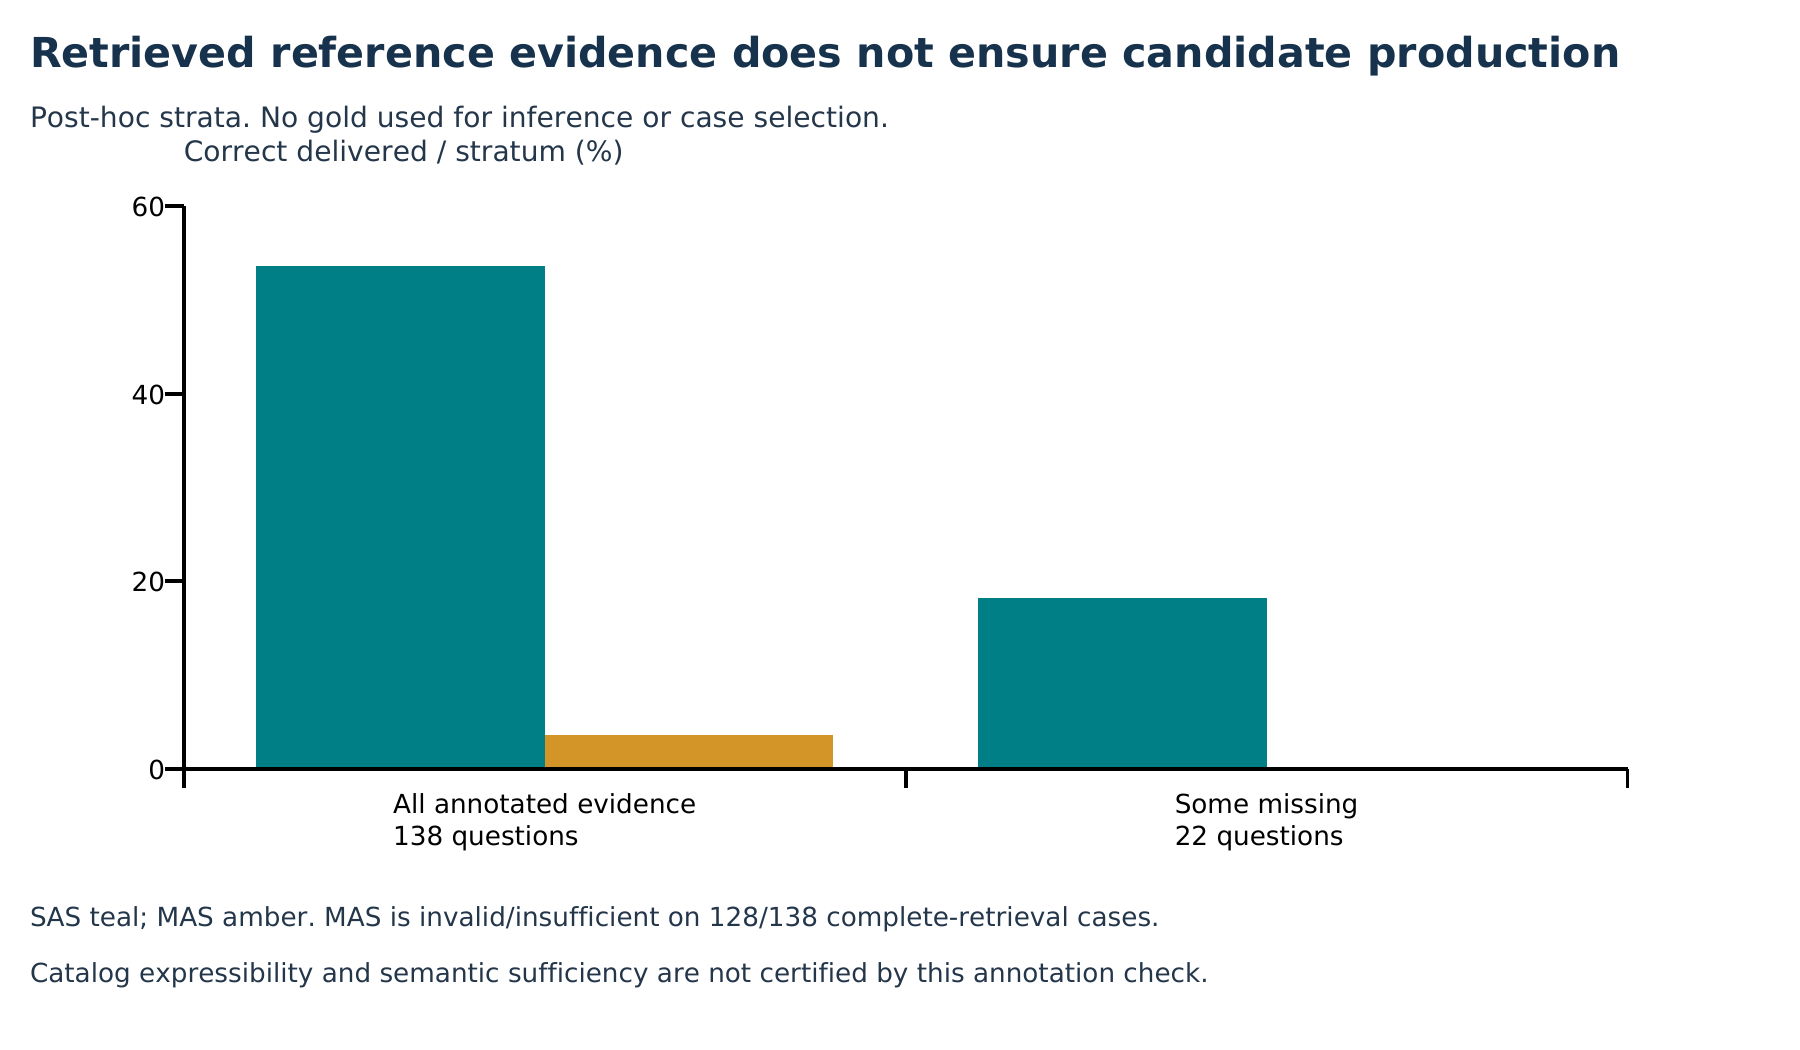
\includegraphics[width=\textwidth,height=0.43\textheight,keepaspectratio]{figures/tier16_v2/10_retrieval_strata.png}
\caption{Correct delivery by annotated retrieval completeness.}
\label{fig:source-13}
\end{figure*}

\subsection{Memory, latency and cost per useful answer}\label{memory-latency-and-cost-per-useful-answer}

\begin{table*}[tbp]
\centering
\setlength{\tabcolsep}{3pt}
\begin{tabular}{@{}>{\raggedright\arraybackslash}p{72.29pt}>{\raggedright\arraybackslash}p{68.05pt}>{\raggedright\arraybackslash}p{71.74pt}>{\raggedright\arraybackslash}p{71.74pt}>{\raggedright\arraybackslash}p{66.14pt}>{\raggedright\arraybackslash}p{48.12pt}>{\raggedright\arraybackslash}p{69.92pt}@{}}
\toprule
\textbf{Arm (primary)} & \textbf{Median s / case} & \textbf{s / reported-correct} & \textbf{Generated tok / case} & \textbf{Prompt tok / case} & \textbf{Peak RSS} & \textbf{Model bytes on disk} \\
\midrule
SAS & 251.4 (mean 259.8) & 532.9 & 204.1 & 4,016.8 & 10.062 GB & 8.99 GB \\
MAS & 53.8 (mean 54.7) & 1,751.4 & 184.4 & 4,666.7 & 10.929 GB & 10.27 GB \\
\bottomrule
\end{tabular}
\caption{Memory, latency and cost per useful answer}
\end{table*}

\textbf{H4 is not supported.} The three-model team used 0.87 GB \emph{more} peak RSS than the monolith, despite having about a third of its parameters, because F16 storage costs about 3.3× more bytes per weight than Q4\_K\_M (≈4.9 effective bits). MAS was 4.75× faster per question. Because it answered so few, it needed 3.29× more inference time per correct answer.

The analysis stage dominates generated tokens in both arms. It reached its 128-token allowance in 159 SAS and 157 MAS cases, which is by design and not a truncation of final JSON. In SAS, program generation dominates wall time, because a 14B model processes about 2,400-token prompts slowly on 8 CPU threads.

\begin{figure*}[tbp]
\centering
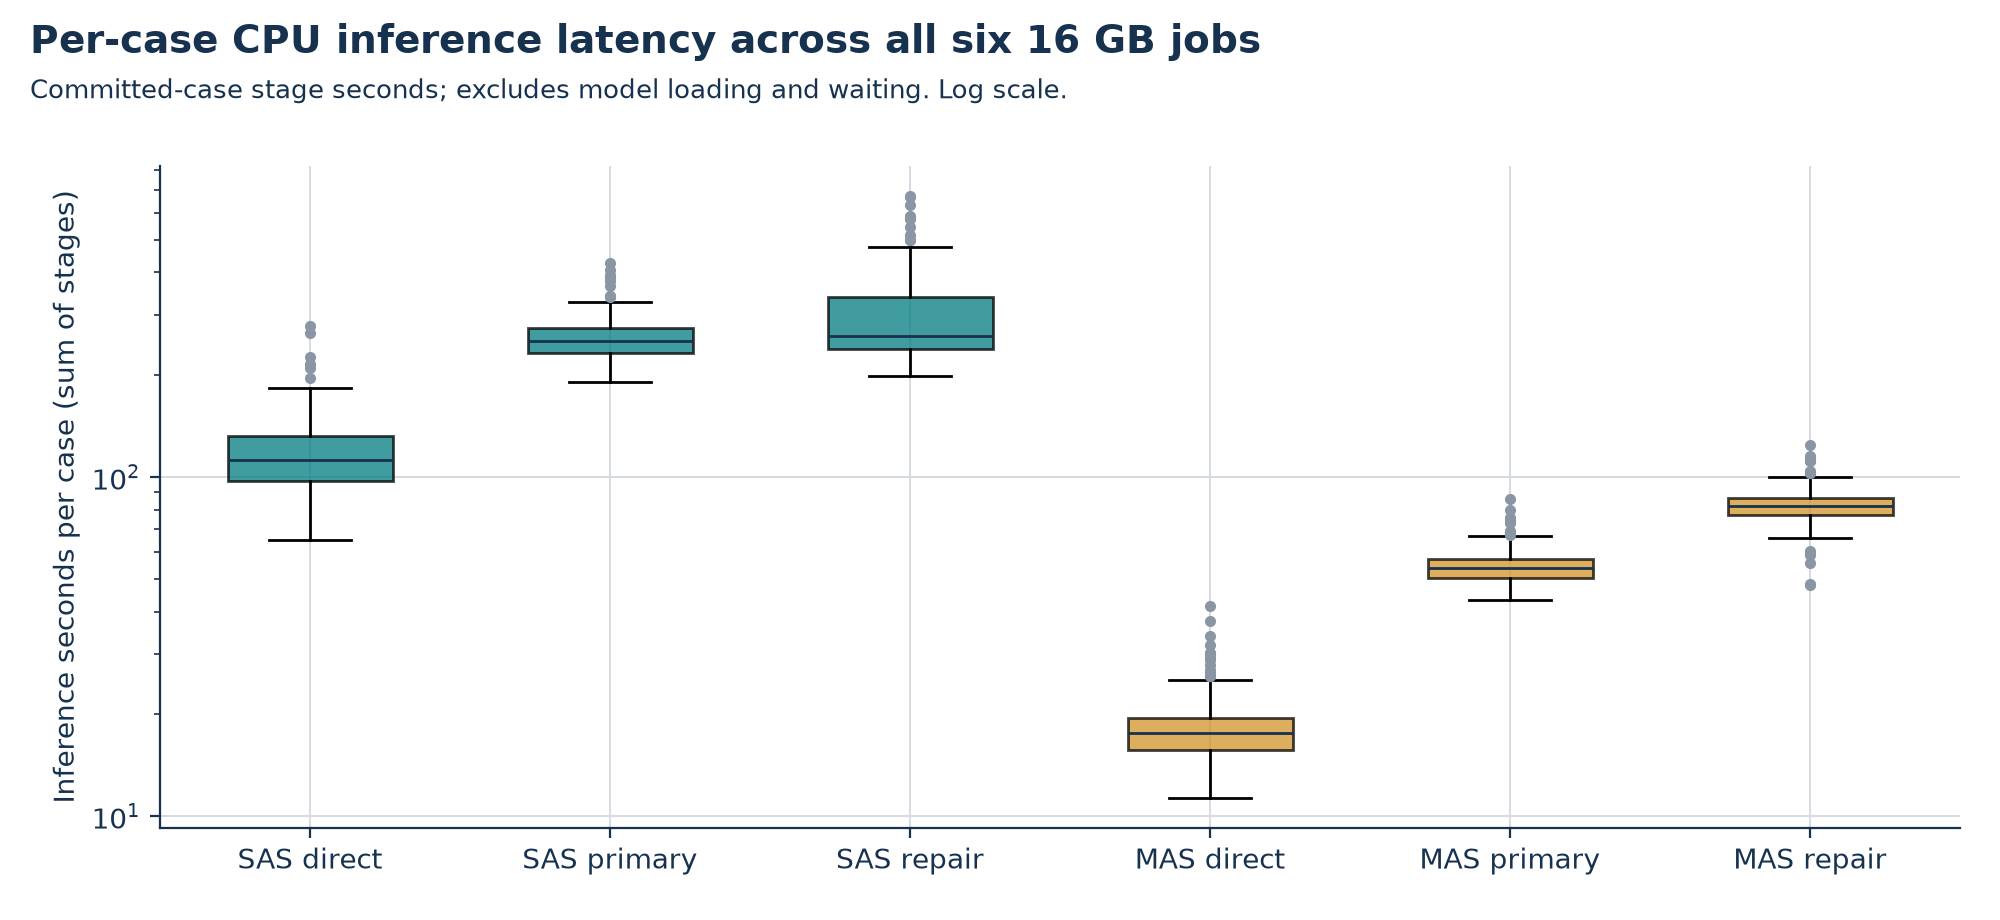
\includegraphics[width=\textwidth,height=0.43\textheight,keepaspectratio]{figures/paper/P05_latency_distributions.png}
\caption{Per-case latency, all six jobs (log scale).}
\label{fig:source-14}
\end{figure*}

\begin{figure*}[tbp]
\centering
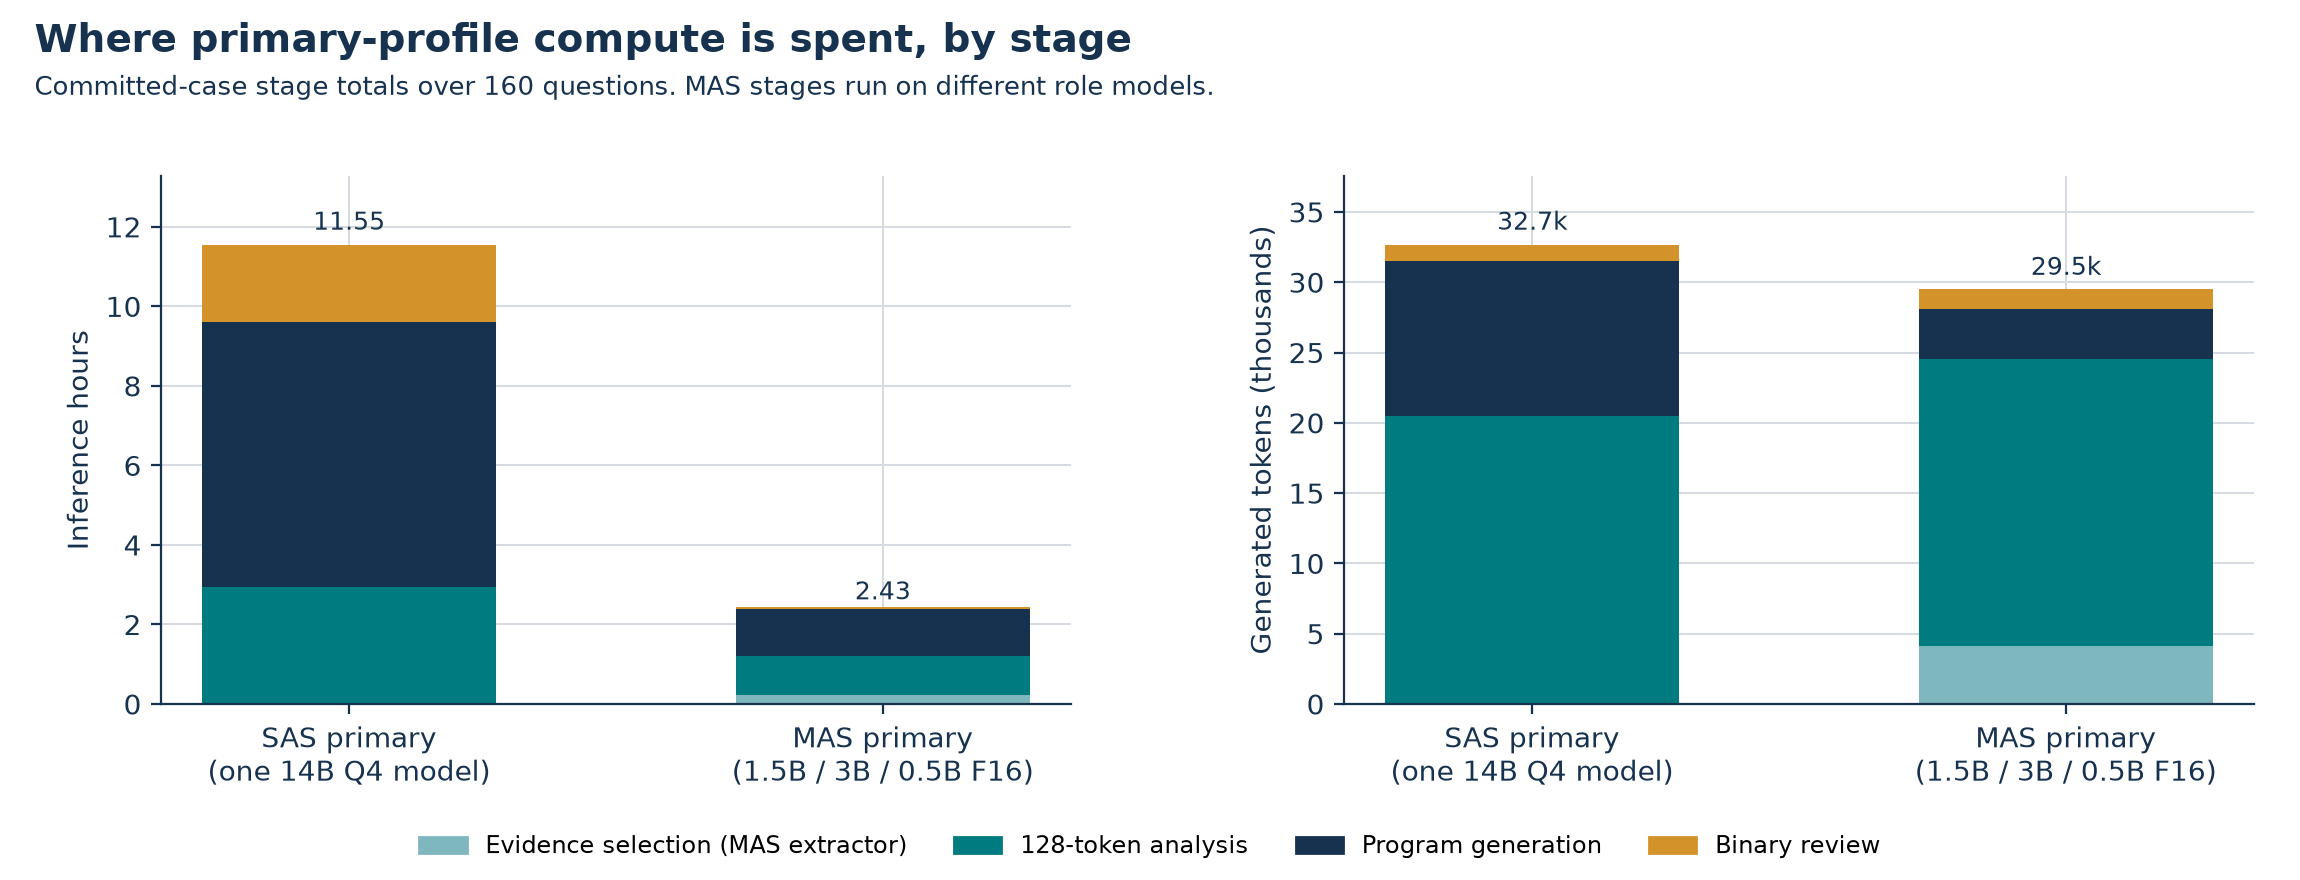
\includegraphics[width=\textwidth,height=0.43\textheight,keepaspectratio]{figures/paper/P07_stage_costs.png}
\caption{Compute by stage.}
\label{fig:source-15}
\end{figure*}

\begin{figure*}[tbp]
\centering
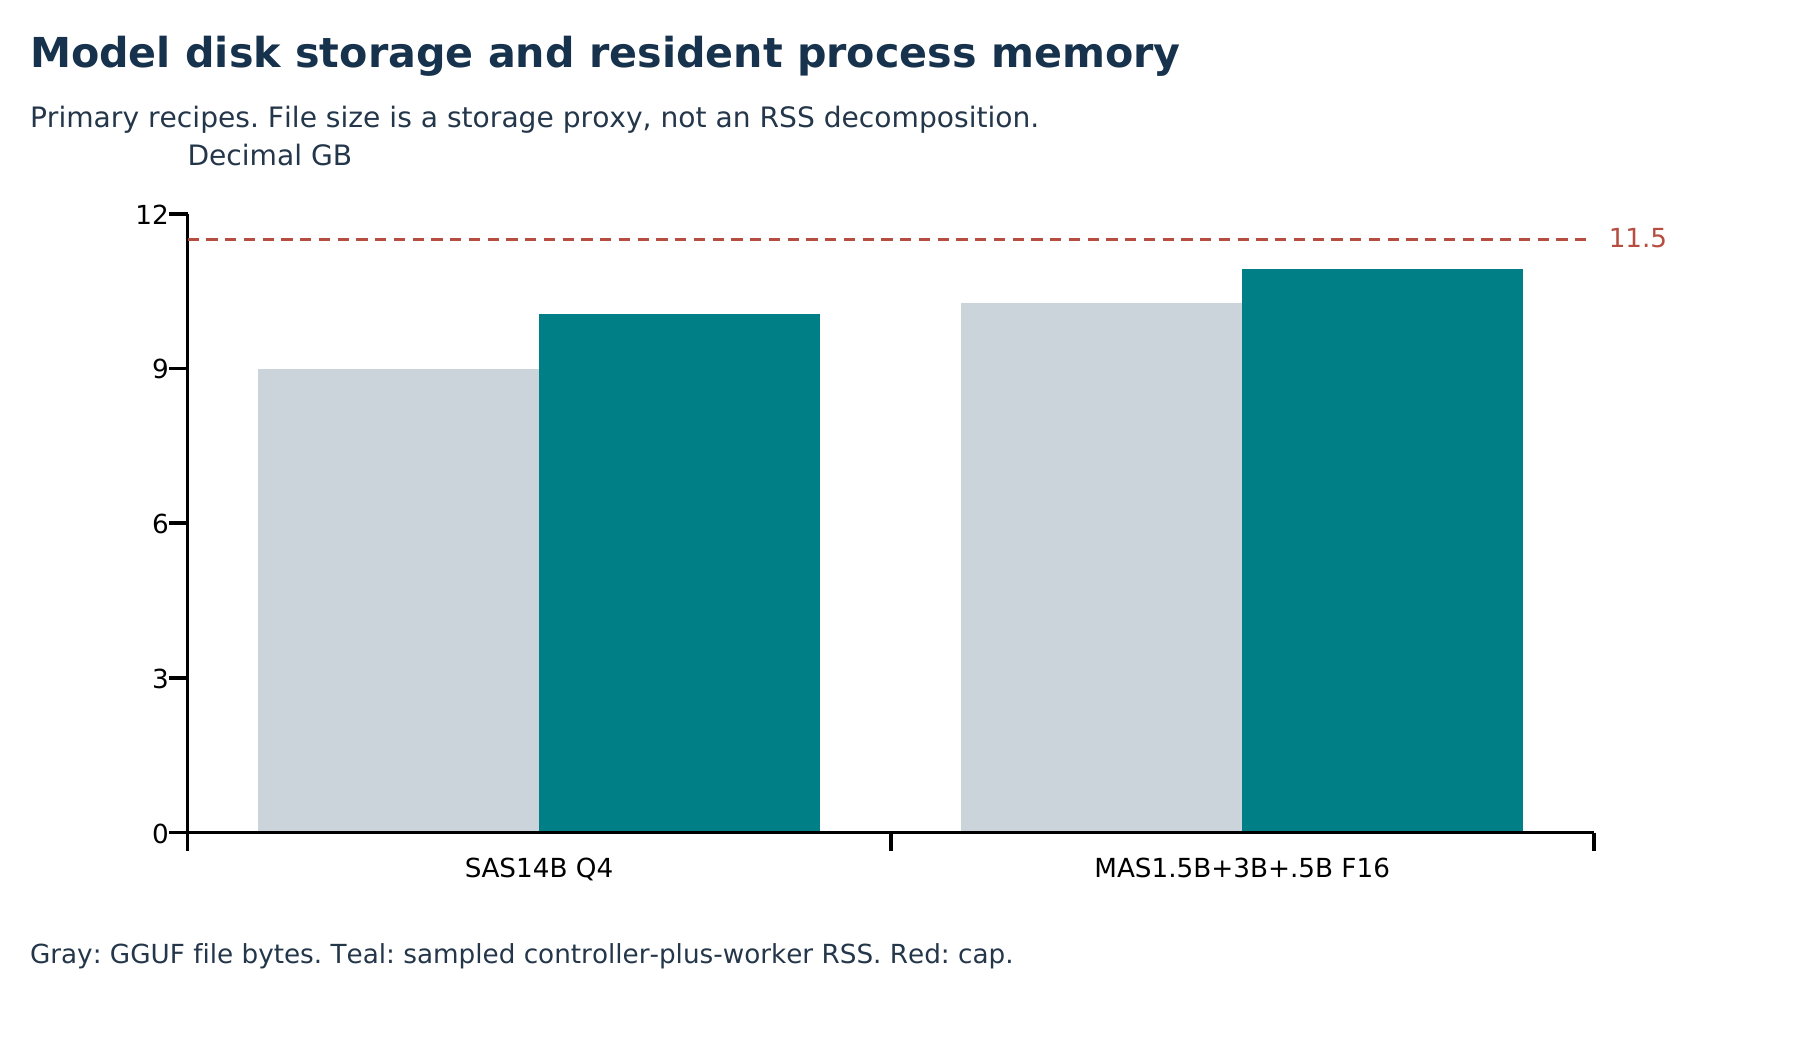
\includegraphics[width=\textwidth,height=0.43\textheight,keepaspectratio]{figures/tier16_v2/12_disk_vs_resident.png}
\caption{Model file size versus sampled resident memory.}
\label{fig:source-16}
\end{figure*}

\begin{figure*}[tbp]
\centering
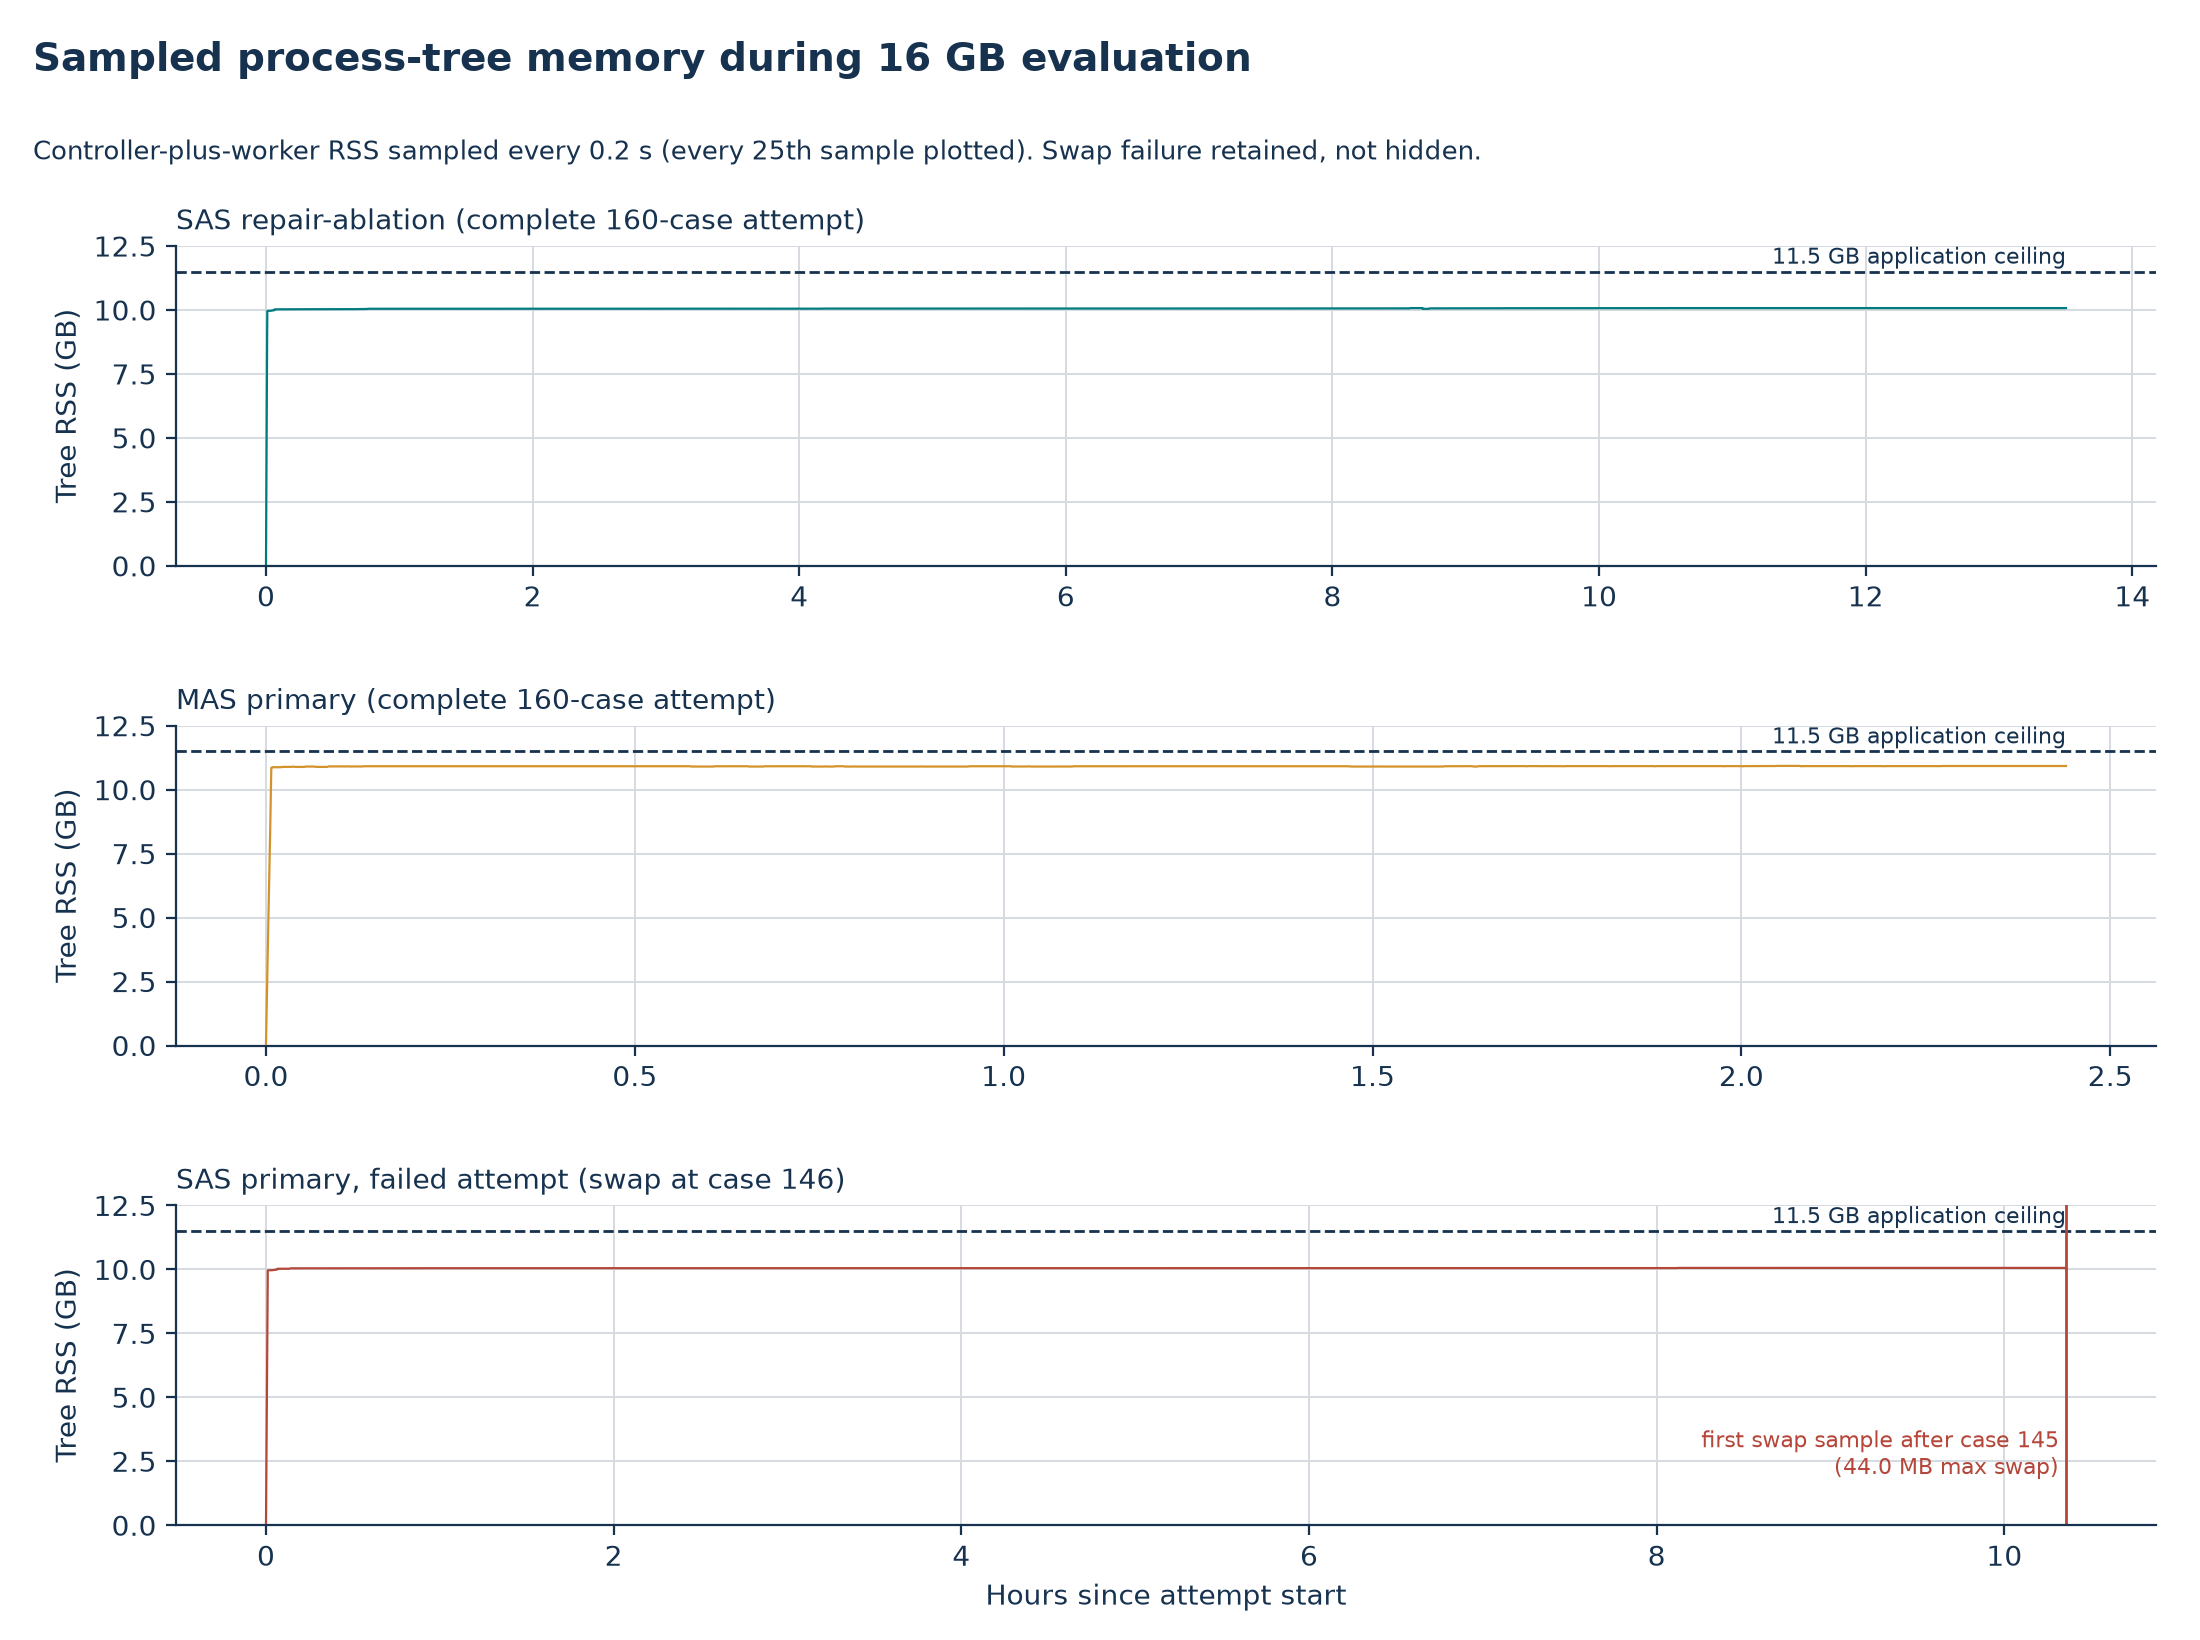
\includegraphics[width=\textwidth,height=0.43\textheight,keepaspectratio]{figures/paper/P06_memory_timelines.png}
\caption{Sampled process-tree RSS over complete attempts and the retained failed attempt.}
\label{fig:source-17}
\end{figure*}

\subsection{Resource validity chronology}\label{resource-validity-chronology}

\begin{enumerate}
\def\labelenumi{\arabic{enumi}.}
\tightlist
\item
  \textbf{Reserve-check stop.} A 12.49 GB-cap attempt stopped at its pre-inference reserve check.
\item
  \textbf{Context reduction.} 8,192-context probes swapped, so context was reduced to 4,096 for both arms.
\item
  \textbf{First swap failure.} The first SAS primary attempt completed 145 cases, then recorded 44,011,520 bytes of process-tree swap while sampled RSS peaked at 10.06 GB, below the ceiling.
\item
  \textbf{First continuation.} A continuation reused the 145 checkpoints that preceded the first invalid sample, after each passed full replay of prompt, program, score, delivery and token ledger. It later swapped 34,430,976 bytes after seven direct-control SAS cases.
\item
  \textbf{Final continuation.} The last run preserved 327 completed cases and ran under a user-systemd service with kernel \path|MemorySwapMax=0|. It completed all six jobs with no further incident.
\end{enumerate}

No case was selected or discarded by quality. The study status is therefore \path|complete_accuracy_audited_resource_invalid|: the accuracy evidence is complete, but it is not an uninterrupted no-swap deployment pass.

\subsection{Utility and decision analysis}\label{utility-and-decision-analysis}

Assign +1 to a correct delivery, −λ to a wrong delivery and −κ to each withheld case (human review cost):

\[U(\lambda,\kappa)=\frac{C-\lambda W-\kappa H}{N}.\]

With κ = 0 and the reported metric, \(U_{SAS}-U_{MAS}=(73-45\lambda)/160\), so MAS is preferred only when λ \textgreater{} 73/45 ≈ 1.62. Above λ = 5/3, MAS utility is itself negative and always-withhold beats both systems. Under the raw metric the switch point is λ = 33/85 ≈ 0.39, because SAS's raw wrong count is large. Pricing human review moves the switch point up: λ* = (73 + 118κ)/45, i.e.~1.88 at κ = 0.1 and 2.28 at κ = 0.25. The region in which the team is the best choice is narrow, and it depends on a loss function that would have to be fixed by the institution in advance rather than read off these data.

\begin{figure*}[tbp]
\centering
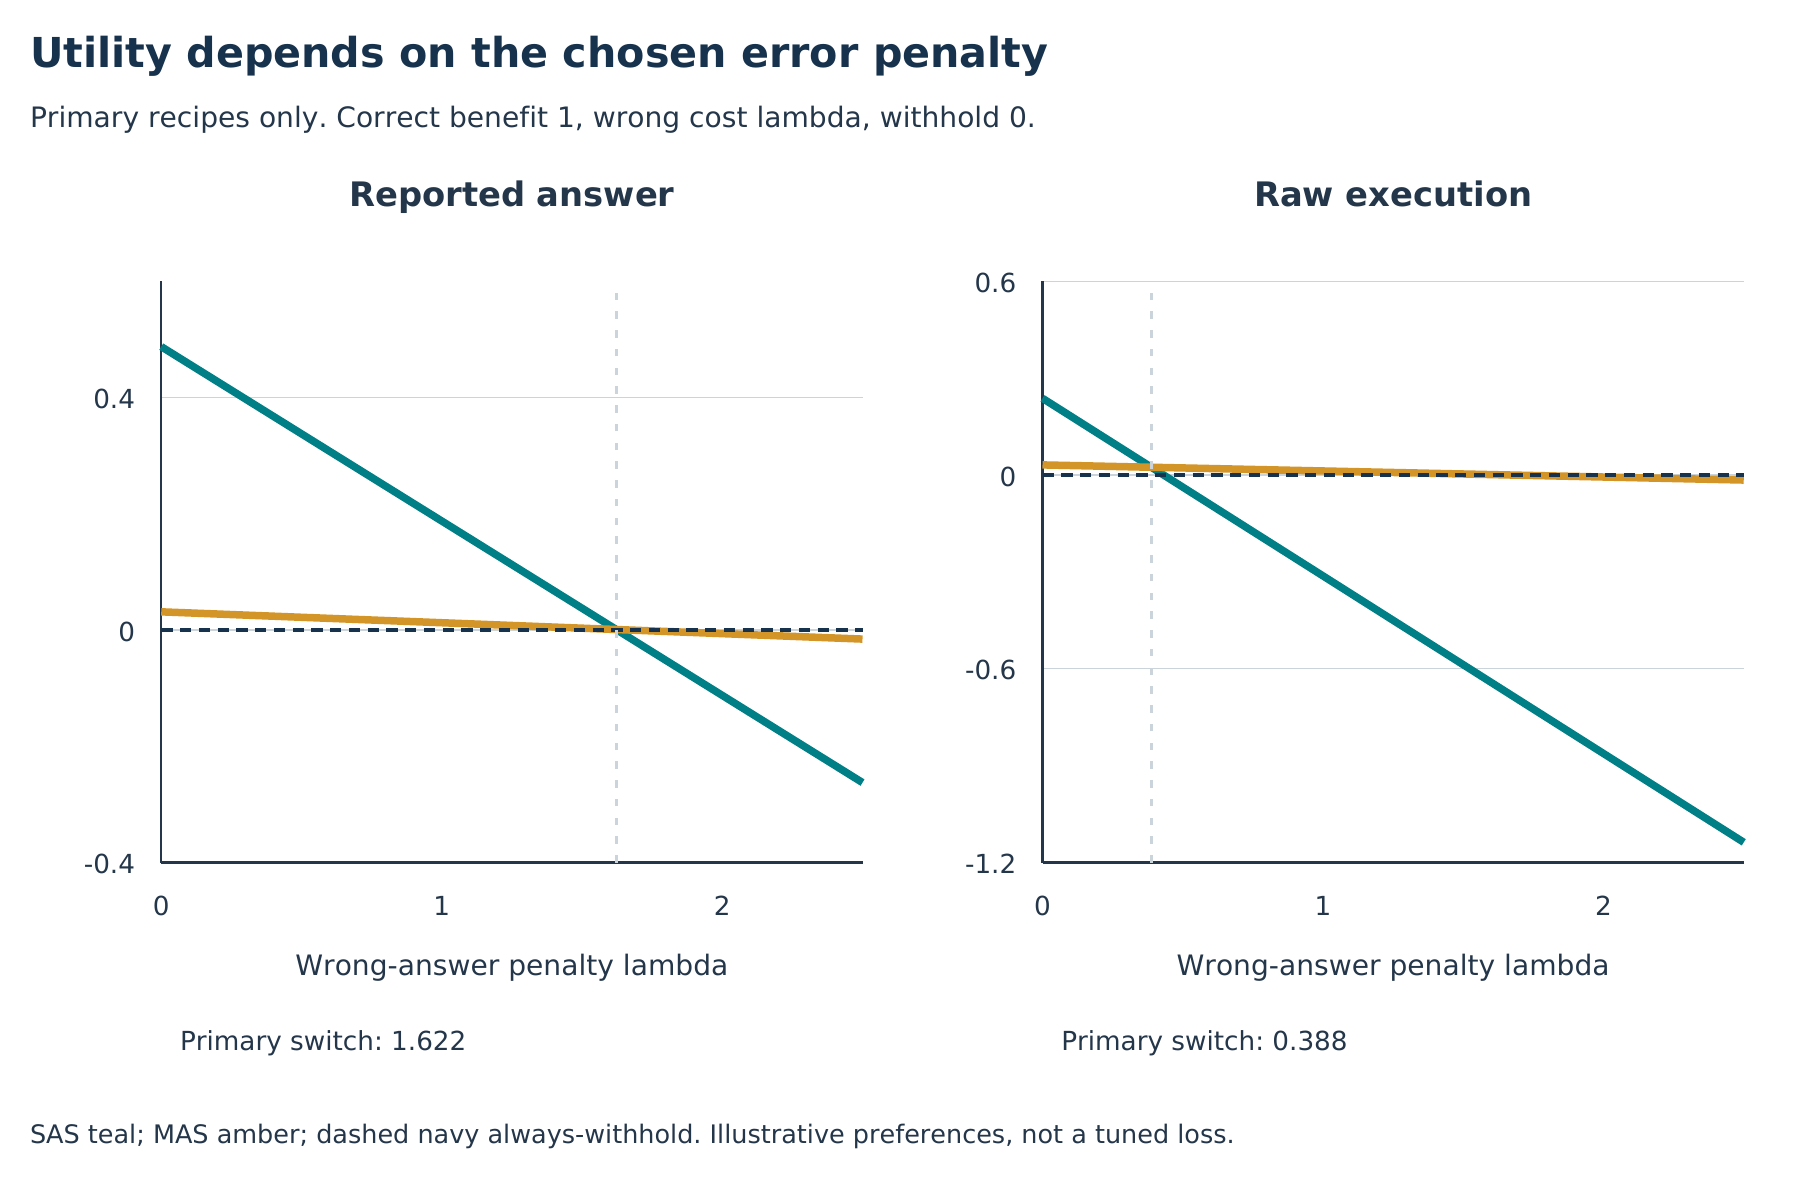
\includegraphics[width=\textwidth,height=0.43\textheight,keepaspectratio]{figures/tier16_v2/08_utility_sensitivity.png}
\caption{Utility versus the wrong-answer penalty.}
\label{fig:source-18}
\end{figure*}

\begin{figure*}[tbp]
\centering
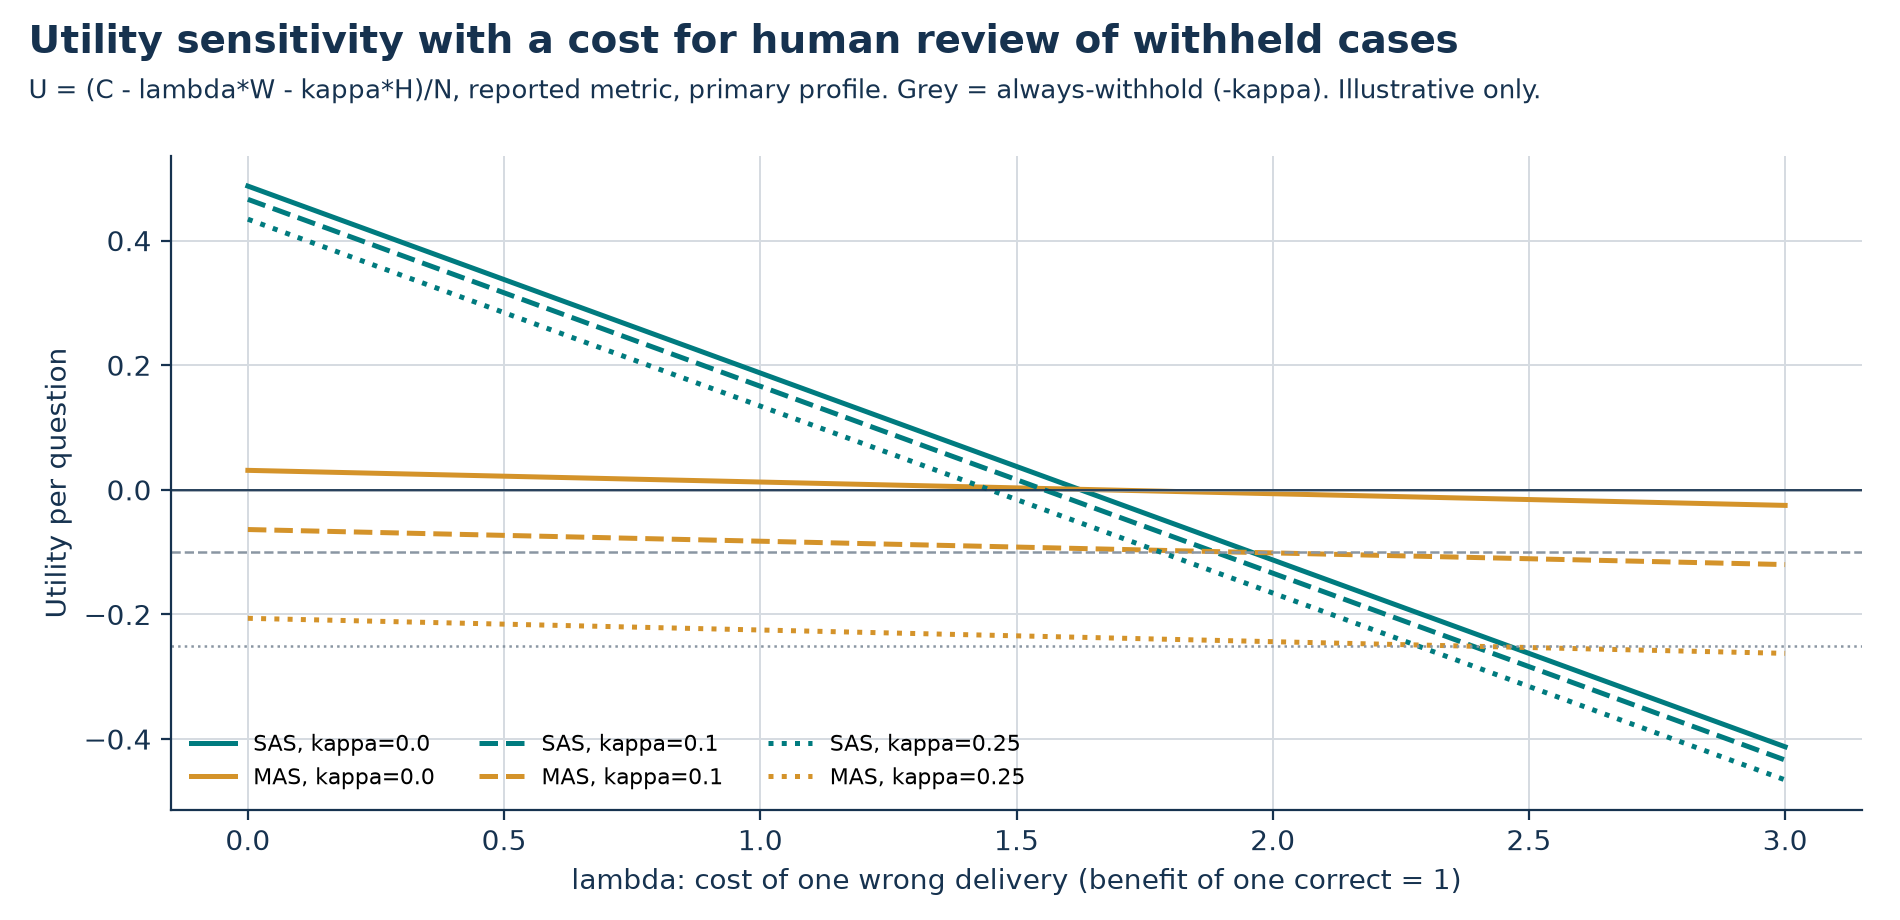
\includegraphics[width=\textwidth,height=0.43\textheight,keepaspectratio]{figures/paper/P09_utility_kappa.png}
\caption{Utility with a cost for human review of withheld cases.}
\label{fig:source-19}
\end{figure*}

\begin{figure*}[tbp]
\centering
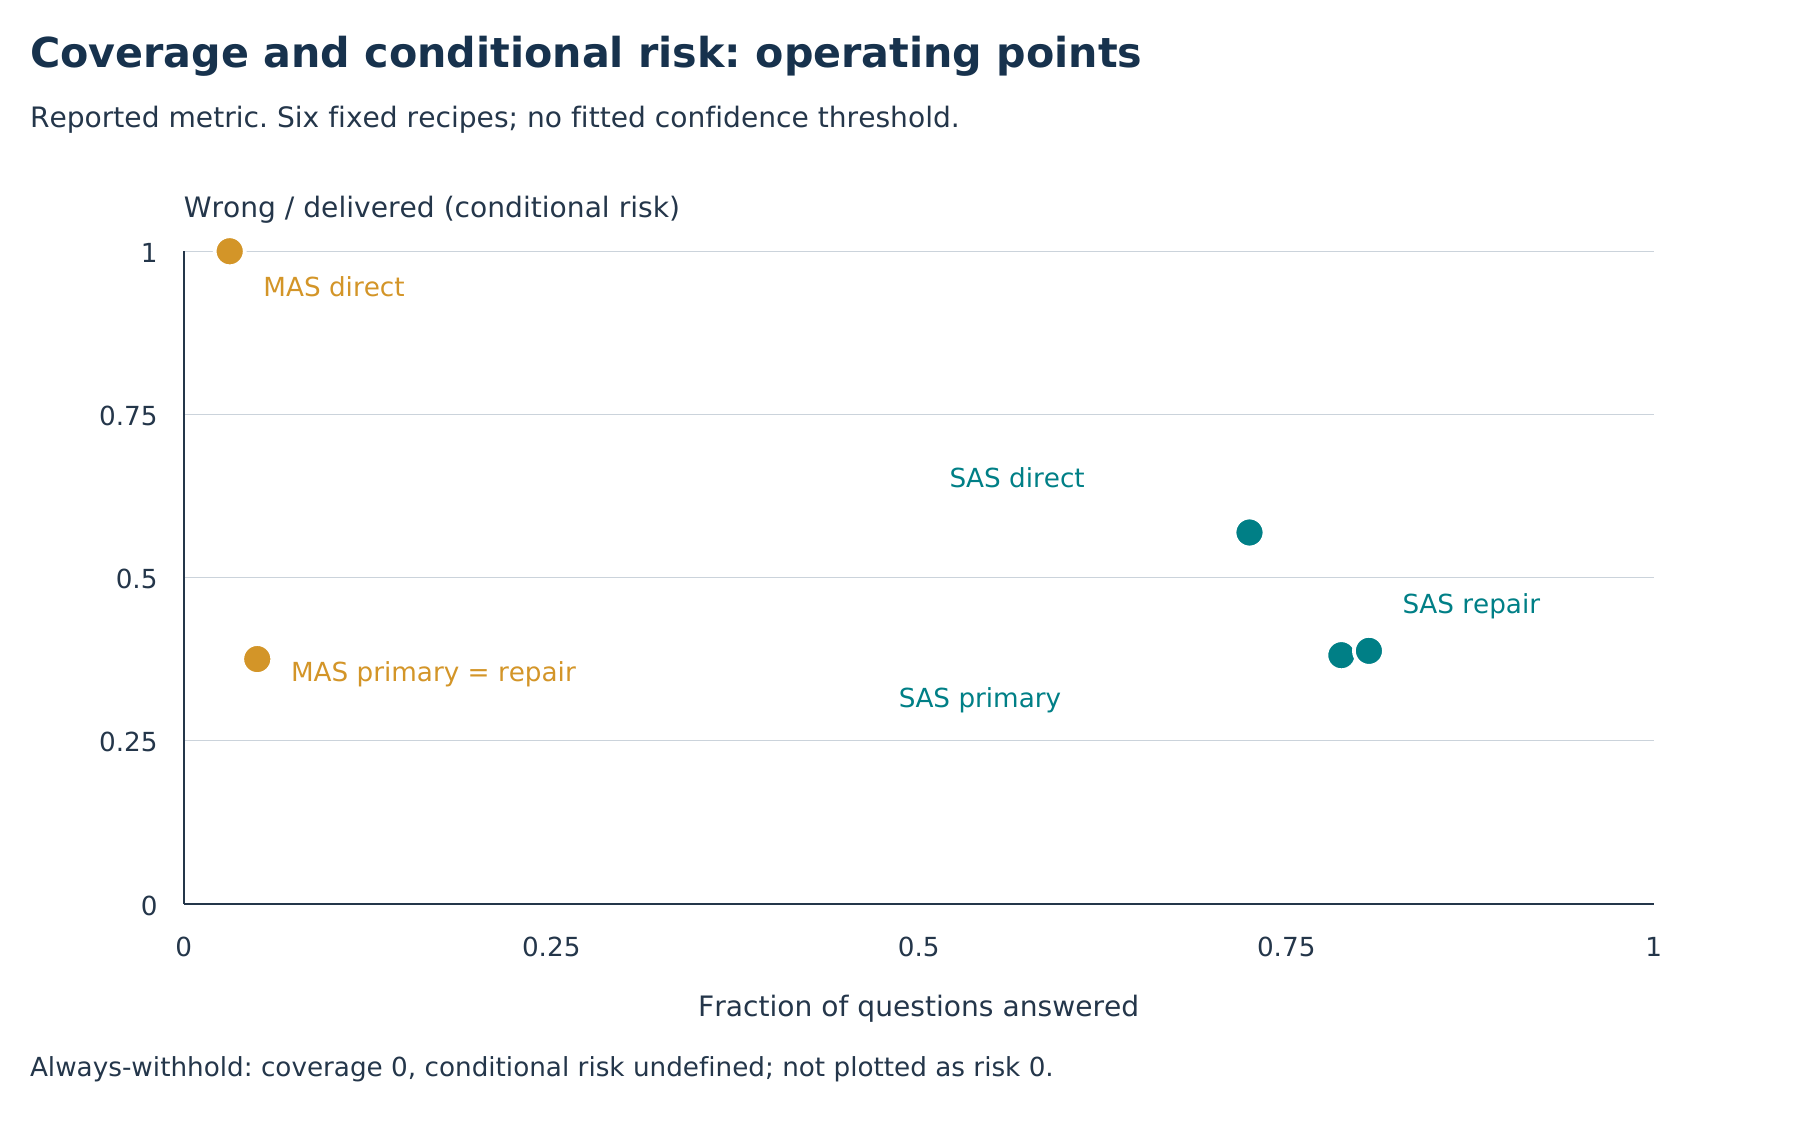
\includegraphics[width=\textwidth,height=0.43\textheight,keepaspectratio]{figures/tier16_v2/07_risk_coverage.png}
\caption{Risk–coverage operating points of the six recipes.}
\label{fig:source-20}
\end{figure*}

\subsection{Numerical hypothesis-test battery}\label{numerical-hypothesis-test-battery}

This subsection applies every test defined in Section 5.9 to the same case-level data. In all tables, b counts questions where the event occurs on the right arm only and c on the left arm only, and Δ is right minus left in percentage points. All values are regenerated by \path|scripts/reporting/paper_statistical_tests.py| (output: \path|research/paper/data/paper_statistical_tests.{json,csv}|, 126 endpoint rows). The recomputed report-cluster bootstrap intervals match the published audit values to every printed digit.

\textbf{Table 6.13a. Primary 16 GB contrast, case-level paired tests (N = 160; case-IID sensitivity).}

\begin{table*}[tbp]
\centering
\setlength{\tabcolsep}{3pt}
\begin{tabular}{@{}>{\raggedright\arraybackslash}p{125.81pt}>{\raggedright\arraybackslash}p{36.35pt}>{\raggedright\arraybackslash}p{36.35pt}>{\raggedright\arraybackslash}p{72.70pt}>{\raggedright\arraybackslash}p{72.70pt}>{\raggedright\arraybackslash}p{51.40pt}>{\raggedright\arraybackslash}p{72.70pt}@{}}
\toprule
\textbf{Endpoint (MAS − SAS)} & \textbf{SAS} & \textbf{MAS} & \textbf{b (MAS only)} & \textbf{c (SAS only)} & \textbf{Δ (pp)} & \textbf{Wald SE (pp)} \\
\midrule
Reported / correct & 78 & 5 & 0 & 73 & −45.62 & 3.94 \\
Reported / wrong & 48 & 3 & 1 & 46 & −28.12 & 3.66 \\
Raw / correct & 38 & 5 & 1 & 34 & −20.62 & 3.32 \\
Raw / wrong & 88 & 3 & 0 & 85 & −53.12 & 3.95 \\
Withheld (both metrics) & 34 & 152 & 118 & 0 & +73.75 & 3.48 \\
\bottomrule
\end{tabular}
\caption{Numerical hypothesis-test battery (column panel 1 of 2)}
\end{table*}

\begin{table*}[tbp]
\centering
\setlength{\tabcolsep}{3pt}
\begin{tabular}{@{}>{\raggedright\arraybackslash}p{107.70pt}>{\raggedright\arraybackslash}p{31.12pt}>{\raggedright\arraybackslash}p{31.12pt}>{\raggedright\arraybackslash}p{71.86pt}>{\raggedright\arraybackslash}p{69.58pt}>{\raggedright\arraybackslash}p{78.31pt}>{\raggedright\arraybackslash}p{78.31pt}@{}}
\toprule
\textbf{Endpoint (MAS − SAS)} & \textbf{SAS} & \textbf{MAS} & \textbf{Wald 95\% CI (pp)} & \textbf{Exact McNemar p} & \textbf{χ² (p)} & \textbf{χ²cc (p)} \\
\midrule
Reported / correct & 78 & 5 & [−53.34, −37.91] & 2.12×10⁻²² & 73.00 (1.30×10⁻¹⁷) & 71.01 (3.55×10⁻¹⁷) \\
Reported / wrong & 48 & 3 & [−35.30, −20.95] & 6.82×10⁻¹³ & 43.09 (5.24×10⁻¹¹) & 41.19 (1.38×10⁻¹⁰) \\
Raw / correct & 38 & 5 & [−27.13, −14.12] & 2.10×10⁻⁹ & 31.11 (2.43×10⁻⁸) & 29.26 (6.34×10⁻⁸) \\
Raw / wrong & 88 & 3 & [−60.86, −45.39] & 5.17×10⁻²⁶ & 85.00 (2.98×10⁻²⁰) & 83.01 (8.16×10⁻²⁰) \\
Withheld (both metrics) & 34 & 152 & [+66.93, +80.57] & 6.02×10⁻³⁶ & 118.00 (1.73×10⁻²⁷) & 116.01 (4.73×10⁻²⁷) \\
\bottomrule
\end{tabular}
\caption{Numerical hypothesis-test battery (column panel 2 of 2)}
\end{table*}

\textbf{Table 6.13b. Primary 16 GB contrast, cluster-aware tests (50 reports; 36 companies).} DEFF is the variance inflation of the CR1 estimator relative to the case-IID variance. The sign-flip Holm values are the published supplemental results; the Durkalski Holm values are added here.

\begin{table*}[tbp]
\centering
\setlength{\tabcolsep}{3pt}
\begin{tabular}{@{}>{\raggedright\arraybackslash}p{106.84pt}>{\raggedright\arraybackslash}p{101.13pt}>{\raggedright\arraybackslash}p{87.58pt}>{\raggedright\arraybackslash}p{83.31pt}>{\raggedright\arraybackslash}p{101.13pt}@{}}
\toprule
\textbf{Endpoint (MAS − SAS)} & \textbf{Report bootstrap 95\% CI (pp)} & \textbf{CR1 SE, report (DEFF)} & \textbf{CR1 z (p)} & \textbf{Durkalski χ², 50 reports (p)} \\
\midrule
Reported / correct & [−53.90, −36.55] & 4.45 (1.28) & −10.25 (1.19×10⁻²⁴) & 24.79 (6.41×10⁻⁷) \\
Reported / wrong & [−37.09, −20.13] & 4.40 (1.45) & −6.39 (1.71×10⁻¹⁰) & 22.75 (1.84×10⁻⁶) \\
Raw / correct & [−28.26, −13.37] & 3.80 (1.31) & −5.42 (5.83×10⁻⁸) & 16.75 (4.26×10⁻⁵) \\
Raw / wrong & [−61.90, −44.08] & 4.57 (1.34) & −11.63 (2.96×10⁻³¹) & 29.25 (6.36×10⁻⁸) \\
Withheld (identity) & [+64.71, +81.93] & 4.42 (1.62) & 16.67 (2.04×10⁻⁶²) & 33.00 (9.24×10⁻⁹) \\
\bottomrule
\end{tabular}
\caption{Numerical hypothesis-test battery (column panel 1 of 2)}
\end{table*}

\begin{table*}[tbp]
\centering
\setlength{\tabcolsep}{3pt}
\begin{tabular}{@{}>{\raggedright\arraybackslash}p{106.35pt}>{\raggedright\arraybackslash}p{104.21pt}>{\raggedright\arraybackslash}p{112.55pt}>{\raggedright\arraybackslash}p{78.44pt}>{\raggedright\arraybackslash}p{78.44pt}@{}}
\toprule
\textbf{Endpoint (MAS − SAS)} & \textbf{Durkalski χ², 36 companies (p)} & \textbf{Reports MAS > / < SAS (sign-test p)} & \textbf{Holm p, sign-flip} & \textbf{Holm p, Durkalski} \\
\midrule
Reported / correct & 14.68 (1.27×10⁻⁴) & 0 / 33 (2.33×10⁻¹⁰) & 6.10×10⁻⁵ & 1.92×10⁻⁶ \\
Reported / wrong & 17.31 (3.18×10⁻⁵) & 1 / 29 (5.77×10⁻⁸) & 6.10×10⁻⁵ & 3.68×10⁻⁶ \\
Raw / correct & 14.92 (1.12×10⁻⁴) & 0 / 21 (9.54×10⁻⁷) & 6.10×10⁻⁵ & 4.26×10⁻⁵ \\
Raw / wrong & 16.16 (5.81×10⁻⁵) & 0 / 41 (9.09×10⁻¹³) & 6.10×10⁻⁵ & 2.54×10⁻⁷ \\
Withheld (identity) & 19.39 (1.06×10⁻⁵) & 43 / 0 (2.27×10⁻¹³) & — & — \\
\bottomrule
\end{tabular}
\caption{Numerical hypothesis-test battery (column panel 2 of 2)}
\end{table*}

\textbf{Table 6.13c. Bowker symmetry and Stuart--Maxwell marginal-homogeneity tests on the 3×3 C/W/H transition tables (16 GB, N = 160 each; case-IID).}

\begin{table*}[tbp]
\centering
\setlength{\tabcolsep}{3pt}
\begin{tabular}{@{}>{\raggedright\arraybackslash}p{146.11pt}>{\raggedright\arraybackslash}p{51.02pt}>{\raggedright\arraybackslash}p{65.03pt}>{\raggedright\arraybackslash}p{57.04pt}>{\raggedright\arraybackslash}p{82.65pt}>{\raggedright\arraybackslash}p{72.15pt}@{}}
\toprule
\textbf{Paired comparison (rows → columns)} & \textbf{Metric} & \textbf{Bowker Q (df)} & \textbf{Bowker p} & \textbf{Stuart–Maxwell Q (df)} & \textbf{Stuart–Maxwell p} \\
\midrule
Primary: MAS vs SAS & Reported & 119.00 (3) & 1.27×10⁻²⁵ & 118.03 (2) & 2.34×10⁻²⁶ \\
Primary: MAS vs SAS & Raw & 119.00 (3) & 1.27×10⁻²⁵ & 118.04 (2) & 2.33×10⁻²⁶ \\
Direct control: MAS vs SAS & Reported & 110.06 (3) & 1.06×10⁻²³ & 109.16 (2) & 1.98×10⁻²⁴ \\
Direct control: MAS vs SAS & Raw & 110.04 (3) & 1.08×10⁻²³ & 109.16 (2) & 1.98×10⁻²⁴ \\
Repair ablation: MAS vs SAS & Reported & 122.00 (3) & 2.86×10⁻²⁶ & 121.03 (2) & 5.22×10⁻²⁷ \\
Repair ablation: MAS vs SAS & Raw & 122.00 (3) & 2.86×10⁻²⁶ & 121.04 (2) & 5.21×10⁻²⁷ \\
SAS: primary vs direct & Reported & 25.15 (3) & 1.44×10⁻⁵ & 22.35 (2) & 1.40×10⁻⁵ \\
SAS: primary vs direct & Raw & 23.29 (3) & 3.52×10⁻⁵ & 23.15 (2) & 9.40×10⁻⁶ \\
MAS: primary vs direct (metrics identical) & Both & 5.50 (2) & 0.064 & 5.50 (2) & 0.064 \\
SAS: repair vs primary & Reported & 3.00 (2) & 0.22 & 3.00 (2) & 0.22 \\
\bottomrule
\end{tabular}
\caption{Numerical hypothesis-test battery (rows 1-10)}
\end{table*}

\begin{table*}[tbp]
\centering
\setlength{\tabcolsep}{3pt}
\begin{tabular}{@{}>{\raggedright\arraybackslash}p{143.66pt}>{\raggedright\arraybackslash}p{43.44pt}>{\raggedright\arraybackslash}p{63.94pt}>{\raggedright\arraybackslash}p{50.16pt}>{\raggedright\arraybackslash}p{101.87pt}>{\raggedright\arraybackslash}p{70.93pt}@{}}
\toprule
\textbf{Paired comparison (rows → columns)} & \textbf{Metric} & \textbf{Bowker Q (df)} & \textbf{Bowker p} & \textbf{Stuart–Maxwell Q (df)} & \textbf{Stuart–Maxwell p} \\
\midrule
SAS: repair vs primary & Raw & 3.00 (1) & 0.083 & 3.00 (1) & 0.083 \\
MAS: repair vs primary (metrics identical) & Both & 0 (0) & — & not defined (no discordant pairs) & — \\
\bottomrule
\end{tabular}
\caption{Numerical hypothesis-test battery (rows 11-12)}
\end{table*}

\textbf{Table 6.13d. Secondary 16 GB paired contrasts (exploratory, unadjusted).} ``Both'' means the two scoring conventions give identical tables.

\begin{table*}[tbp]
\centering
\setlength{\tabcolsep}{3pt}
\begin{tabular}{@{}>{\raggedright\arraybackslash}p{123.99pt}>{\raggedright\arraybackslash}p{54.00pt}>{\raggedright\arraybackslash}p{54.00pt}>{\raggedright\arraybackslash}p{66.13pt}>{\raggedright\arraybackslash}p{46.76pt}>{\raggedright\arraybackslash}p{46.76pt}>{\raggedright\arraybackslash}p{76.36pt}@{}}
\toprule
\textbf{Contrast (right − left)} & \textbf{Metric} & \textbf{Endpoint} & \textbf{Left → right} & \textbf{b / c} & \textbf{Δ (pp)} & \textbf{Wald 95\% CI} \\
\midrule
Direct control: MAS vs SAS & Reported & correct & 50 → 0 & 0 / 50 & −31.25 & [−38.43, −24.07] \\
Direct control: MAS vs SAS & Reported & wrong & 66 → 5 & 2 / 63 & −38.12 & [−46.04, −30.21] \\
Direct control: MAS vs SAS & Raw & correct & 14 → 0 & 0 / 14 & −8.75 & [−13.13, −4.37] \\
Direct control: MAS vs SAS & Raw & wrong & 102 → 5 & 2 / 99 & −60.62 & [−68.58, −52.67] \\
Repair ablation: MAS vs SAS & Reported & correct & 79 → 5 & 0 / 74 & −46.25 & [−53.98, −38.52] \\
Repair ablation: MAS vs SAS & Reported & wrong & 50 → 3 & 1 / 48 & −29.38 & [−36.64, −22.11] \\
Repair ablation: MAS vs SAS & Raw & correct & 38 → 5 & 1 / 34 & −20.62 & [−27.13, −14.12] \\
Repair ablation: MAS vs SAS & Raw & wrong & 91 → 3 & 0 / 88 & −55.00 & [−62.71, −47.29] \\
SAS: primary vs direct & Reported & correct & 50 → 78 & 32 / 4 & +17.50 & [+10.67, +24.33] \\
SAS: primary vs direct & Reported & wrong & 66 → 48 & 9 / 27 & −11.25 & [−18.39, −4.11] \\
\bottomrule
\end{tabular}
\caption{Numerical hypothesis-test battery (column panel 1 of 2) (rows 1-10)}
\end{table*}

\begin{table*}[tbp]
\centering
\setlength{\tabcolsep}{3pt}
\begin{tabular}{@{}>{\raggedright\arraybackslash}p{116.49pt}>{\raggedright\arraybackslash}p{54.96pt}>{\raggedright\arraybackslash}p{54.96pt}>{\raggedright\arraybackslash}p{67.31pt}>{\raggedright\arraybackslash}p{51.41pt}>{\raggedright\arraybackslash}p{47.60pt}>{\raggedright\arraybackslash}p{75.26pt}@{}}
\toprule
\textbf{Contrast (right − left)} & \textbf{Metric} & \textbf{Endpoint} & \textbf{Left → right} & \textbf{b / c} & \textbf{Δ (pp)} & \textbf{Wald 95\% CI} \\
\midrule
SAS: primary vs direct & Raw & correct & 14 → 38 & 27 / 3 & +15.00 & [+8.71, +21.29] \\
SAS: primary vs direct & Raw & wrong & 102 → 88 & 15 / 29 & −8.75 & [−16.76, −0.74] \\
MAS: primary vs direct & Both & correct & 0 → 5 & 5 / 0 & +3.12 & [+0.43, +5.82] \\
MAS: primary vs direct & Both & wrong & 5 → 3 & 3 / 5 & −1.25 & [−4.71, +2.21] \\
SAS: repair vs primary & Reported & correct & 78 → 79 & 1 / 0 & +0.62 & [−0.60, +1.85] \\
SAS: repair vs primary & Reported & wrong & 48 → 50 & 2 / 0 & +1.25 & [−0.47, +2.97] \\
SAS: repair vs primary & Raw & correct & 38 → 38 & 0 / 0 & 0.00 & [0.00, 0.00] \\
SAS: repair vs primary & Raw & wrong & 88 → 91 & 3 / 0 & +1.88 & [−0.23, +3.98] \\
MAS: repair vs primary & Both & correct & 5 → 5 & 0 / 0 & 0.00 & [0.00, 0.00] \\
MAS: repair vs primary & Both & wrong & 3 → 3 & 0 / 0 & 0.00 & [0.00, 0.00] \\
\bottomrule
\end{tabular}
\caption{Numerical hypothesis-test battery (column panel 1 of 2) (rows 11-20)}
\end{table*}

\begin{table*}[tbp]
\centering
\setlength{\tabcolsep}{3pt}
\begin{tabular}{@{}>{\raggedright\arraybackslash}p{131.42pt}>{\raggedright\arraybackslash}p{57.23pt}>{\raggedright\arraybackslash}p{57.23pt}>{\raggedright\arraybackslash}p{97.04pt}>{\raggedright\arraybackslash}p{63.98pt}>{\raggedright\arraybackslash}p{67.11pt}@{}}
\toprule
\textbf{Contrast (right − left)} & \textbf{Metric} & \textbf{Endpoint} & \textbf{Report bootstrap 95\% CI} & \textbf{Exact p} & \textbf{Durkalski p} \\
\midrule
Direct control: MAS vs SAS & Reported & correct & [−40.12, −22.63] & 1.78×10⁻¹⁵ & 5.01×10⁻⁶ \\
Direct control: MAS vs SAS & Reported & wrong & [−47.65, −29.05] & 1.16×10⁻¹⁶ & 4.87×10⁻⁷ \\
Direct control: MAS vs SAS & Raw & correct & [−13.29, −4.74] & 1.22×10⁻⁴ & 4.65×10⁻⁴ \\
Direct control: MAS vs SAS & Raw & wrong & [−70.18, −50.63] & 4.06×10⁻²⁷ & 4.19×10⁻⁸ \\
Repair ablation: MAS vs SAS & Reported & correct & [−54.67, −37.06] & 1.06×10⁻²² & 6.07×10⁻⁷ \\
Repair ablation: MAS vs SAS & Reported & wrong & [−38.41, −21.38] & 1.78×10⁻¹³ & 8.35×10⁻⁷ \\
Repair ablation: MAS vs SAS & Raw & correct & [−28.26, −13.37] & 2.10×10⁻⁹ & 4.26×10⁻⁵ \\
Repair ablation: MAS vs SAS & Raw & wrong & [−63.93, −45.86] & 6.46×10⁻²⁷ & 3.80×10⁻⁸ \\
SAS: primary vs direct & Reported & correct & [+9.76, +24.55] & 1.94×10⁻⁶ & 4.65×10⁻⁴ \\
SAS: primary vs direct & Reported & wrong & [−17.98, −3.90] & 0.004 & 0.007 \\
\bottomrule
\end{tabular}
\caption{Numerical hypothesis-test battery (column panel 2 of 2) (rows 1-10)}
\end{table*}

\begin{table*}[tbp]
\centering
\setlength{\tabcolsep}{3pt}
\begin{tabular}{@{}>{\raggedright\arraybackslash}p{124.83pt}>{\raggedright\arraybackslash}p{58.89pt}>{\raggedright\arraybackslash}p{58.89pt}>{\raggedright\arraybackslash}p{99.86pt}>{\raggedright\arraybackslash}p{62.47pt}>{\raggedright\arraybackslash}p{69.06pt}@{}}
\toprule
\textbf{Contrast (right − left)} & \textbf{Metric} & \textbf{Endpoint} & \textbf{Report bootstrap 95\% CI} & \textbf{Exact p} & \textbf{Durkalski p} \\
\midrule
SAS: primary vs direct & Raw & correct & [+8.59, +21.62] & 8.43×10⁻⁶ & 4.02×10⁻⁴ \\
SAS: primary vs direct & Raw & wrong & [−17.96, +0.72] & 0.049 & 0.080 \\
MAS: primary vs direct & Both & correct & [0.00, +6.98] & 0.0625 & 0.096 \\
MAS: primary vs direct & Both & wrong & [−5.26, +2.55] & 0.73 & 0.53 \\
SAS: repair vs primary & Reported & correct & [0.00, +2.04] & 1.00 & 0.32 \\
SAS: repair vs primary & Reported & wrong & [0.00, +3.40] & 0.50 & 0.16 \\
SAS: repair vs primary & Raw & correct & [0.00, 0.00] & 1.00 & 1.00 \\
SAS: repair vs primary & Raw & wrong & [0.00, +4.35] & 0.25 & 0.083 \\
MAS: repair vs primary & Both & correct & [0.00, 0.00] & 1.00 & 1.00 \\
MAS: repair vs primary & Both & wrong & [0.00, 0.00] & 1.00 & 1.00 \\
\bottomrule
\end{tabular}
\caption{Numerical hypothesis-test battery (column panel 2 of 2) (rows 11-20)}
\end{table*}

\textbf{Table 6.13e. Redeveloped 8 GB paired contrasts, reported metric (exploratory, unadjusted).} Raw-metric rows are in the CSV.

\begin{table*}[tbp]
\centering
\setlength{\tabcolsep}{3pt}
\begin{tabular}{@{}>{\raggedright\arraybackslash}p{135.22pt}>{\raggedright\arraybackslash}p{27.04pt}>{\raggedright\arraybackslash}p{54.09pt}>{\raggedright\arraybackslash}p{66.25pt}>{\raggedright\arraybackslash}p{46.84pt}>{\raggedright\arraybackslash}p{46.84pt}>{\raggedright\arraybackslash}p{91.71pt}@{}}
\toprule
\textbf{8 GB contrast (right − left)} & \textbf{N} & \textbf{Endpoint} & \textbf{Left → right} & \textbf{b / c} & \textbf{Δ (pp)} & \textbf{Report bootstrap 95\% CI} \\
\midrule
Selection52: baseline MAS vs SAS & 52 & correct & 8 → 2 & 0 / 6 & −11.54 & [−23.26, −2.00] \\
Selection52: baseline MAS vs SAS & 52 & wrong & 25 → 19 & 8 / 14 & −11.54 & [−32.56, +7.69] \\
Selection52: control MAS vs SAS & 52 & correct & 8 → 3 & 0 / 5 & −9.62 & [−18.33, −2.00] \\
Selection52: control MAS vs SAS & 52 & wrong & 23 → 19 & 4 / 8 & −7.69 & [−21.82, +9.30] \\
Selection52: crossed MAS vs SAS & 52 & correct & 10 → 3 & 0 / 7 & −13.46 & [−28.85, −2.00] \\
Selection52: crossed MAS vs SAS & 52 & wrong & 16 → 15 & 6 / 7 & −1.92 & [−15.69, +15.26] \\
Reserved49: control MAS vs SAS & 49 & correct & 8 → 4 & 1 / 5 & −8.16 & [−16.22, 0.00] \\
Reserved49: control MAS vs SAS & 49 & wrong & 20 → 17 & 6 / 9 & −6.12 & [−27.27, +10.91] \\
Reserved49: crossed MAS vs SAS & 49 & correct & 9 → 4 & 1 / 6 & −10.20 & [−20.83, 0.00] \\
Reserved49: crossed MAS vs SAS & 49 & wrong & 20 → 9 & 3 / 14 & −22.45 & [−38.71, −7.50] \\
\bottomrule
\end{tabular}
\caption{Numerical hypothesis-test battery (column panel 1 of 2) (rows 1-10)}
\end{table*}

\begin{table*}[tbp]
\centering
\setlength{\tabcolsep}{3pt}
\begin{tabular}{@{}>{\raggedright\arraybackslash}p{162.66pt}>{\raggedright\arraybackslash}p{24.81pt}>{\raggedright\arraybackslash}p{49.63pt}>{\raggedright\arraybackslash}p{60.78pt}>{\raggedright\arraybackslash}p{42.98pt}>{\raggedright\arraybackslash}p{42.98pt}>{\raggedright\arraybackslash}p{84.15pt}@{}}
\toprule
\textbf{8 GB contrast (right − left)} & \textbf{N} & \textbf{Endpoint} & \textbf{Left → right} & \textbf{b / c} & \textbf{Δ (pp)} & \textbf{Report bootstrap 95\% CI} \\
\midrule
Selection52: crossed vs control MAS & 52 & correct & 3 → 3 & 0 / 0 & 0.00 & [0.00, 0.00] \\
Selection52: crossed vs control MAS & 52 & wrong & 19 → 15 & 1 / 5 & −7.69 & [−17.74, +2.08] \\
Selection52: crossed vs original-critic MAS & 52 & correct & 4 → 3 & 0 / 1 & −1.92 & [−5.77, 0.00] \\
Selection52: crossed vs original-critic MAS & 52 & wrong & 22 → 15 & 3 / 10 & −13.46 & [−25.00, −1.85] \\
Reserved49: crossed vs control MAS & 49 & correct & 4 → 4 & 0 / 0 & 0.00 & [0.00, 0.00] \\
Reserved49: crossed vs control MAS & 49 & wrong & 17 → 9 & 2 / 10 & −16.33 & [−26.23, −4.26] \\
Selection52: crossed vs control SAS & 52 & correct & 8 → 10 & 2 / 0 & +3.85 & [0.00, +11.54] \\
Selection52: crossed vs control SAS & 52 & wrong & 23 → 16 & 4 / 11 & −13.46 & [−26.79, 0.00] \\
Selection52: crossed vs control SAS (analysis128+demos) & 52 & correct & 9 → 9 & 1 / 1 & 0.00 & [0.00, 0.00] \\
Selection52: crossed vs control SAS (analysis128+demos) & 52 & wrong & 20 → 10 & 3 / 13 & −19.23 & [−38.03, −2.08] \\
\bottomrule
\end{tabular}
\caption{Numerical hypothesis-test battery (column panel 1 of 2) (rows 11-20)}
\end{table*}

\begin{table*}[tbp]
\centering
\setlength{\tabcolsep}{3pt}
\begin{tabular}{@{}>{\raggedright\arraybackslash}p{163.00pt}>{\raggedright\arraybackslash}p{25.10pt}>{\raggedright\arraybackslash}p{50.19pt}>{\raggedright\arraybackslash}p{61.47pt}>{\raggedright\arraybackslash}p{39.68pt}>{\raggedright\arraybackslash}p{43.47pt}>{\raggedright\arraybackslash}p{85.10pt}@{}}
\toprule
\textbf{8 GB contrast (right − left)} & \textbf{N} & \textbf{Endpoint} & \textbf{Left → right} & \textbf{b / c} & \textbf{Δ (pp)} & \textbf{Report bootstrap 95\% CI} \\
\midrule
Reserved49: crossed vs control SAS & 49 & correct & 8 → 9 & 1 / 0 & +2.04 & [0.00, +5.56] \\
Reserved49: crossed vs control SAS & 49 & wrong & 20 → 20 & 3 / 3 & 0.00 & [−10.64, +8.62] \\
Selection52: baseline SAS, analysis128+demos vs direct & 52 & correct & 8 → 9 & 2 / 1 & +1.92 & [−4.26, +8.77] \\
Selection52: baseline SAS, analysis128+demos vs direct & 52 & wrong & 25 → 24 & 5 / 6 & −1.92 & [−12.07, +12.50] \\
Selection52: control SAS, analysis128+demos vs direct & 52 & correct & 8 → 9 & 2 / 1 & +1.92 & [−5.41, +10.53] \\
Selection52: control SAS, analysis128+demos vs direct & 52 & wrong & 23 → 20 & 4 / 7 & −5.77 & [−18.75, +6.82] \\
Selection52: crossed SAS, analysis128+demos vs direct & 52 & correct & 10 → 9 & 0 / 1 & −1.92 & [−6.25, 0.00] \\
Selection52: crossed SAS, analysis128+demos vs direct & 52 & wrong & 16 → 10 & 2 / 8 & −11.54 & [−27.27, 0.00] \\
\bottomrule
\end{tabular}
\caption{Numerical hypothesis-test battery (column panel 1 of 2) (rows 21-28)}
\end{table*}

\begin{table*}[tbp]
\centering
\setlength{\tabcolsep}{3pt}
\begin{tabular}{@{}>{\raggedright\arraybackslash}p{141.84pt}>{\raggedright\arraybackslash}p{28.37pt}>{\raggedright\arraybackslash}p{56.74pt}>{\raggedright\arraybackslash}p{53.07pt}>{\raggedright\arraybackslash}p{49.13pt}>{\raggedright\arraybackslash}p{66.53pt}>{\raggedright\arraybackslash}p{72.32pt}@{}}
\toprule
\textbf{8 GB contrast (right − left)} & \textbf{N} & \textbf{Endpoint} & \textbf{Exact p} & \textbf{χ²cc p} & \textbf{Durkalski p} & \textbf{Bowker p (df)} \\
\midrule
Selection52: baseline MAS vs SAS & 52 & correct & 0.031 & 0.041 & 0.083 & 0.027 (3) \\
Selection52: baseline MAS vs SAS & 52 & wrong & 0.29 & 0.29 & 0.26 & 0.027 (3) \\
Selection52: control MAS vs SAS & 52 & correct & 0.0625 & 0.074 & 0.059 & 0.064 (3) \\
Selection52: control MAS vs SAS & 52 & wrong & 0.39 & 0.39 & 0.37 & 0.064 (3) \\
Selection52: crossed MAS vs SAS & 52 & correct & 0.016 & 0.023 & 0.11 & 0.062 (3) \\
Selection52: crossed MAS vs SAS & 52 & wrong & 1.00 & 1.00 & 0.81 & 0.062 (3) \\
Reserved49: control MAS vs SAS & 49 & correct & 0.22 & 0.22 & 0.10 & 0.18 (3) \\
Reserved49: control MAS vs SAS & 49 & wrong & 0.61 & 0.61 & 0.51 & 0.18 (3) \\
Reserved49: crossed MAS vs SAS & 49 & correct & 0.12 & 0.13 & 0.13 & 0.005 (3) \\
Reserved49: crossed MAS vs SAS & 49 & wrong & 0.013 & 0.015 & 0.022 & 0.005 (3) \\
\bottomrule
\end{tabular}
\caption{Numerical hypothesis-test battery (column panel 2 of 2) (rows 1-10)}
\end{table*}

\begin{table*}[tbp]
\centering
\setlength{\tabcolsep}{3pt}
\begin{tabular}{@{}>{\raggedright\arraybackslash}p{169.93pt}>{\raggedright\arraybackslash}p{25.92pt}>{\raggedright\arraybackslash}p{51.85pt}>{\raggedright\arraybackslash}p{48.50pt}>{\raggedright\arraybackslash}p{44.90pt}>{\raggedright\arraybackslash}p{60.80pt}>{\raggedright\arraybackslash}p{66.09pt}@{}}
\toprule
\textbf{8 GB contrast (right − left)} & \textbf{N} & \textbf{Endpoint} & \textbf{Exact p} & \textbf{χ²cc p} & \textbf{Durkalski p} & \textbf{Bowker p (df)} \\
\midrule
Selection52: crossed vs control MAS & 52 & correct & 1.00 & 1.00 & 1.00 & 0.10 (1) \\
Selection52: crossed vs control MAS & 52 & wrong & 0.22 & 0.22 & 0.16 & 0.10 (1) \\
Selection52: crossed vs original-critic MAS & 52 & correct & 1.00 & 1.00 & 0.32 & 0.092 (2) \\
Selection52: crossed vs original-critic MAS & 52 & wrong & 0.092 & 0.096 & 0.052 & 0.092 (2) \\
Reserved49: crossed vs control MAS & 49 & correct & 1.00 & 1.00 & 1.00 & 0.021 (1) \\
Reserved49: crossed vs control MAS & 49 & wrong & 0.039 & 0.043 & 0.046 & 0.021 (1) \\
Selection52: crossed vs control SAS & 52 & correct & 0.50 & 0.48 & 0.32 & 0.14 (2) \\
Selection52: crossed vs control SAS & 52 & wrong & 0.12 & 0.12 & 0.11 & 0.14 (2) \\
Selection52: crossed vs control SAS (analysis128+demos) & 52 & correct & 1.00 & 1.00 & 1.00 & 0.060 (3) \\
Selection52: crossed vs control SAS (analysis128+demos) & 52 & wrong & 0.021 & 0.024 & 0.068 & 0.060 (3) \\
\bottomrule
\end{tabular}
\caption{Numerical hypothesis-test battery (column panel 2 of 2) (rows 11-20)}
\end{table*}

\begin{table*}[tbp]
\centering
\setlength{\tabcolsep}{3pt}
\begin{tabular}{@{}>{\raggedright\arraybackslash}p{168.94pt}>{\raggedright\arraybackslash}p{26.01pt}>{\raggedright\arraybackslash}p{52.02pt}>{\raggedright\arraybackslash}p{48.66pt}>{\raggedright\arraybackslash}p{45.05pt}>{\raggedright\arraybackslash}p{61.00pt}>{\raggedright\arraybackslash}p{66.31pt}@{}}
\toprule
\textbf{8 GB contrast (right − left)} & \textbf{N} & \textbf{Endpoint} & \textbf{Exact p} & \textbf{χ²cc p} & \textbf{Durkalski p} & \textbf{Bowker p (df)} \\
\midrule
Reserved49: crossed vs control SAS & 49 & correct & 1.00 & 1.00 & 0.32 & 0.61 (2) \\
Reserved49: crossed vs control SAS & 49 & wrong & 1.00 & 1.00 & 1.00 & 0.61 (2) \\
Selection52: baseline SAS, analysis128+demos vs direct & 52 & correct & 1.00 & 1.00 & 0.56 & 0.80 (3) \\
Selection52: baseline SAS, analysis128+demos vs direct & 52 & wrong & 1.00 & 1.00 & 0.76 & 0.80 (3) \\
Selection52: control SAS, analysis128+demos vs direct & 52 & correct & 1.00 & 1.00 & 0.65 & 0.37 (3) \\
Selection52: control SAS, analysis128+demos vs direct & 52 & wrong & 0.55 & 0.55 & 0.41 & 0.37 (3) \\
Selection52: crossed SAS, analysis128+demos vs direct & 52 & correct & 1.00 & 1.00 & 0.32 & 0.040 (2) \\
Selection52: crossed SAS, analysis128+demos vs direct & 52 & wrong & 0.11 & 0.11 & 0.13 & 0.040 (2) \\
\bottomrule
\end{tabular}
\caption{Numerical hypothesis-test battery (column panel 2 of 2) (rows 21-28)}
\end{table*}

\textbf{Reading the battery.}

\begin{enumerate}
\def\labelenumi{\arabic{enumi}.}
\tightlist
\item
  \textbf{The primary result survives every test.} All four prespecified endpoints reject the null under every procedure: case-IID exact and asymptotic, report- and company-clustered, sign-based, and Holm-adjusted under two different cluster tests. The largest Holm-adjusted cluster-aware p-value is 6.1×10⁻⁵, well below 0.05. The direction is unambiguous: MAS was higher on 0 of 33 discordant reports for reported-correct delivery and on 0 of 21 for raw-correct delivery.
\item
  \textbf{Ignoring clustering overstates the evidence by many orders of magnitude, but does not change the conclusion.} For reported-correct delivery the case-IID exact McNemar gives p = 2.1×10⁻²², the report-level Durkalski test 6.4×10⁻⁷ and the company-level test 1.3×10⁻⁴. The report-level design effects of 1.28--1.62 mean that the 160 questions carry roughly the information of 99--125 independent questions (160/DEFF). Proposition 10 shows that, with 50 reports, no cluster-adjusted McNemar p-value could ever approach the case-IID value. Case-IID p-values are therefore reported only as sensitivity diagnostics.
\item
  \textbf{The 3×3 tables locate the asymmetry.} The reported-metric Bowker statistic decomposes exactly as 1 (C↔W) + 72 (C↔H) + 46 (W↔H) = 119, and the raw-metric statistic as 1 + 34 + 84 = 119. Almost all asymmetry runs from a SAS delivery to a MAS withholding, and none runs the other way. Stuart--Maxwell confirms that the marginal C/W/H distributions differ (Q ≈ 118, 2 df).
\item
  \textbf{Architecture contrasts replicate across profiles.} Direct-control and repair-ablation MAS-versus-SAS contrasts reproduce the primary pattern, with all cluster-adjusted p-values below 5×10⁻⁴.
\item
  \textbf{The prompt bundle effect is robust for SAS correct delivery, but not for every endpoint.} SAS primary versus direct gives +17.5 pp reported-correct (32 versus 4 discordant; Durkalski p = 4.7×10⁻⁴). The SAS raw wrong-delivery reduction is a boundary case: the case-IID exact p = 0.049, but the cluster-adjusted p = 0.080 and the bootstrap interval crosses zero. Under standard 3 it is not claimed.
\item
  \textbf{Some ``non-significant'' results are structurally non-significant.} The MAS bundle moved 5 questions to correct and none away (5/0). Its exact p = 0.0625 is the smallest value attainable with five discordant pairs (Proposition 9), so no test could have been significant at α = 0.05. The Wald interval {[}+0.43, +5.82{]} excludes zero there, which illustrates why Wald intervals are descriptive only. The MAS repair contrast has no discordant pair at all: the null is met exactly in sample, and every test statistic is degenerate.
\item
  \textbf{The 8 GB evidence is consistent in direction but individually weak.} In all five 8 GB SAS/MAS architecture pairs, MAS gained at most one correct delivery that SAS missed (b ≤ 1). Five of 28 reported-metric endpoint tests reach unadjusted exact p \textless{} 0.05, and two do so under the cluster-adjusted test. None survives Holm adjustment over the 28: the smallest adjusted value is 0.36. The sole MAS critic result that is significant under both tests (reserved crossed versus control, wrong deliveries 17 → 9, exact p = 0.039, Durkalski p = 0.046) left correct deliveries unchanged at 4 → 4. By Proposition 1 it is therefore a shift into withholding, not an accuracy gain. These overlapping-condition pairs share questions and models and are not independent replications.
\end{enumerate}

\section{Example Outputs}\label{example-outputs}

All examples come from saved responses in run \path|lab-16-115gb-recovery-02| (16 GB) or \path|tier8-8gb-v1| (8 GB). Text in quotation marks and JSON objects is copied verbatim, with ``\ldots{}'' marking truncation. Unquoted lines (for example ``eight chained subtractions'' or \path|divide(A004=16944, ...)|) are our compact descriptions of the saved program, and timings, executor values and verdicts are taken from the saved trace. Evidence packets are abbreviated.

\subsection{Both arms correct: ABMD/2007/page\_52.pdf-1}\label{both-arms-correct-abmd2007page_52.pdf-1}

\emph{Question:} ``What is the total possible purchase price for Impella including potential contingent payments, in millions?'' Gold: 56.3 = add(11.2, 45.1). Relevant catalog entries: \path|A013=45.1@text_3|, \path|A017=11.2@text_4|.

\begin{lstlisting}
MAS extractor (1.5B, 5.3 s):  {"source_ids": ["text_3", "text_4", "text_5", "text_6"]}
MAS drafter analysis (3B, 128 tok, 21.6 s, verbatim excerpt):
  "Let's define the variables:
   - \( P \): Total purchase price excluding contingent payment
   - \( C \): Contingent payment ...
   - \( P = 45.1 \) million (from text_3)
   - \( C = 11.2 \) million (from text_4) ...
   \[ T = P + C \] ..."
MAS drafter program (3B, 30.1 s):
  {"decision": "ANSWER", "answer_unit": "number", "steps": [{"op": "add", "left": "A013", "right": "A017"}]}
Executor: 56.3, spans [text_3, text_4]      MAS verifier (0.5B, 1.3 s): {"verdict": "PASS"}  → delivered, correct

SAS (14B Q4): identical program {"op":"add","left":"A013","right":"A017"}; program stage 144.1 s,
              review 39.0 s → PASS → delivered, correct
\end{lstlisting}

The two arms produce identical programs; the team is about 4× faster on this question (58.3 s versus 249.3 s of total inference).

\subsection{SAS correct, MAS abstains: AAPL/2003/page\_24.pdf-1}\label{sas-correct-mas-abstains-aapl2003page_24.pdf-1}

\emph{Question:} ``What were capital expenditures associated with the retail segment since its inception, exclusive of the amount incurred during 2003, in millions?'' Gold: 198 = 290 − 92, both values in one sentence (\path|text_16|).

\begin{lstlisting}
SAS program:  {"decision":"ANSWER","answer_unit":"number","steps":[{"op":"subtract","left":"A005","right":"A007"}]}
              → 290 − 92 = 198, review PASS → delivered, correct
MAS extractor: {"source_ids": ["text_16", "text_17", "text_18"]}   (correct sentence selected)
MAS analysis:  "The requested financial measures are capital expenditures associated with the retail
                segment since its inception, excluding the amount incurred during 2003 ..."
MAS program:   {"decision": "INSUFFICIENT", "answer_unit": "number", "steps": []}
MAS verifier:  {"verdict": "FAIL"} → withheld
\end{lstlisting}

The extractor found the right evidence and the analysis restated the task correctly, yet the 3B drafter declined to write a one-step program. This is the dominant MAS failure: 72 questions where SAS was correct and MAS withheld.

\subsection{SAS wrong (accepted by its reviewer), MAS operand error caught: AAPL/2003/page\_24.pdf-2}\label{sas-wrong-accepted-by-its-reviewer-mas-operand-error-caught-aapl2003page_24.pdf-2}

\emph{Question:} ``What was the greatest gross margin percentage in the three year period?'' Gold: 27.9 (\path|table_max|).

\begin{lstlisting}
SAS program (180 tokens): eight chained subtractions over A003..A007 and #0..#5
              → executes to 6.1; 14B review: {"verdict": "PASS"} → delivered, WRONG
MAS program:  {"decision":"ANSWER","answer_unit":"percent","steps":[{"op":"divide","left":"A009","right":"A010"}]}
              → 27 ÷ 2003 = 0.0135 (a year used as an operand)
MAS verifier: {"verdict": "FAIL"} → withheld
\end{lstlisting}

The program grammar has no \path|max| operation, so this ``table aggregate'' question is hard to express. Here SAS's reviewer accepted a meaningless program. Section 6.6 shows that the 14B reviewer accepted 73\% of wrong executable candidates.

\subsection{Team reviewer passes a nonsensical program: PNC/2018/page\_171.pdf-1}\label{team-reviewer-passes-a-nonsensical-program-pnc2018page_171.pdf-1}

\emph{Question:} ``In 2018 what was the percent of the total commitments to extend credit and other commitments for home equity lines of credit?'' Gold: 9.3\% = 16944 / 181612.

\begin{lstlisting}
SAS:  divide(A004=16944, A000=181612) × CONST:100 → 9.33 (percent), PASS → delivered, correct
MAS:  divide(31@text_4, 169278@table_6) × 100 ÷ 169278 → 1.08e-7 (fraction)
      0.5B verifier: {"verdict": "PASS"} → delivered, WRONG
\end{lstlisting}

This is the single question where SAS was correct and MAS delivered a wrong answer. The 0.5B verifier's PASS on an implausible value illustrates the acquiescent verification also seen at 8 GB.

\subsection{Historical 8 GB credit pack: CR-TEST-0001 (synthetic)}\label{historical-8-gb-credit-pack-cr-test-0001-synthetic}

Source lines (abridged): \path|L02 operating_profit_pkr=52852800|; \path|L03 annual_debt_service_pkr=13000000; current_assets_pkr=211000000; current_liabilities_pkr=70000000|; \path|L04 e-CIB status=ADVERSE_LINE_REVIEW_REQUIRED; last_review_date=NOT_PROVIDED|. The label requires \path|e_cib_last_review_date = MISSING|.

\begin{lstlisting}
SAS (7B Q4, 97.4 s, 364 tokens): valid JSON; DSCR 4.0656 [CALC#DSCR], current ratio 3.0143
   [CALC#CURRENT_RATIO], e_cib_status from L04 — all verified; e_cib_last_review_date = "NOT_PROVIDED" [L04]
   → scored as "invented field" (copied sentinel instead of MISSING); failure tag S6
MAS (62.7 s, 735 tokens): extractor emitted fenced ```json ...```; drafter output also fenced and
   cited non-existent spans (CALC#STATUS, CALC#LAST_REVIEW_DATE) → invalid JSON, failure tag M2
\end{lstlisting}

\section{Formal Framework (Conditional Propositions)}\label{formal-framework-conditional-propositions}

The following are elementary identities and bounds applied to the audit. They are stated with their assumptions, are not claimed as new theorems, and do not prove universal architecture rankings.

\subsection{Decision and accounting propositions}\label{decision-and-accounting-propositions}

\textbf{P1. Accounting identity.} For each metric, \(C+W+H=N\) and \(\Delta C+\Delta W+\Delta H=0\). Fewer wrong answers can be bought by withholding; always-withhold gives \(W=0\) and \(C=0\). \emph{Proof:} sum the mutually exclusive per-case indicators.

\textbf{P2. Fixed-candidate gate bound.} If a gate can only accept or reject a fixed candidate, then with \(A\) the set of correct candidates and \(D\) the delivered set, \(C_{\text{gate}}=|A\cap D|\le|A|\). For the primary MAS candidates, \(|A|=5\). \emph{No} reviewer, however good, could have delivered more than 5/160 correct answers from these drafts, against 78 delivered by SAS. The bound does not apply to a new generator or representation.

\textbf{P3. Stage decomposition.} \(C/N=q\,p\,a\), \(W/N=q(1-p)b\) and \(H/N=1-C/N-W/N\), by the chain rule and without any independence assumption. Substituting the observed values reproduces the counts exactly (Section 6.6).

\textbf{P4. Utility switch points.} \(U_{SAS}-U_{MAS}=(73-45\lambda+118\kappa)/160\) (reported), so \(\lambda^*=(73+118\kappa)/45\); for raw, \(\lambda^*=(33+118\kappa)/85\). These are preference statements, not discovered safety thresholds.

\textbf{P5. Repair break-even.} SAS repair changes reported utility by \((1-2\lambda)/160\) and raw utility by \(-3\lambda/160\). MAS repair changes neither. Any positive compute cost makes repair worse still in this sample.

\textbf{P6. Memory arithmetic.} For distinct, fully resident tensors with \(n_j\) elements at \(b_j\) effective bits, \(M\ge\sum_j n_j b_j/8+M_{KV}+M_{\text{other}}\), and a genuinely shared tensor is counted once. The parameter count alone therefore does not order memory when precisions differ. Observed: 8.99 GB on disk / 10.06 GB RSS (SAS) versus 10.27 / 10.93 GB (MAS).

\textbf{P7. Distribution-free cluster bound.} With independent report contributions \(D_g\in[-1,1]\) and fixed weights \(w_g=n_g/N\), Hoeffding's inequality gives \begin{figure*}[tbp]
\[\begin{gathered}\Pr\Big(\big|\textstyle\sum_g w_g(D_g-\mathbb{E}D_g)\big|\ge\varepsilon\Big)\le 2\exp\!\Big(-\frac{\varepsilon^2}{2\sum_g w_g^2}\Big),\; G_{\text{eff}}=\frac{1}{\sum_g w_g^2}.\end{gathered}\]
\end{figure*} Here \(G_{\text{eff}}=36.99\) (reports) and \(19.88\) (companies). The 95\% half-width is 44.7 pp (52.4 pp for a four-contrast family; 60.9 pp with company grouping). The observed −45.6 pp correct-delivery contrast just exceeds the single-contrast half-width but not the family-wise or company-level ones. This deliberately assumption-light bound therefore gives only borderline support on its own, and the tighter intervals in Section 6.5 rely on the bootstrap's stronger assumptions.

\textbf{P8. Metric disagreement.} \(C_{\text{rep}}-C_{\text{raw}}=R_{\text{only}}-E_{\text{only}}\). For SAS, \(78-38=44-4\).

\textbf{Nonidentification.} RAM, checkpoint size, adaptation, serving backend, prompt profile and question source all change between regimes. Many response functions with different RAM slopes therefore reproduce the same observations, and no cross-tier regression can identify a RAM effect. Similarly, a Markov ``error cascade'' argument requires that downstream roles receive information only through the handoff, which is false here because every role sees the evidence packet.

\subsection{Theoretical justification of the testing standards}\label{theoretical-justification-of-the-testing-standards}

Each argument below explains why a test in Section 5.9 answers the question we ask of it, what it assumes, and where it fails. All are standard results (McNemar, 1947; Bowker, 1948; Stuart, 1955; Maxwell, 1970; Durkalski et al., 2003; Agresti, 2013) applied to this design. Two short propositions (P9, P10) make the consequences for this study explicit.

\textbf{J1. Why the tests must be paired.} Both arms answer the same questions, so the per-question outcomes are correlated. For the paired difference, \[\operatorname{Var}(\hat\Delta)=\frac{1}{N}\Big[\pi_R(1-\pi_R)+\pi_L(1-\pi_L)-2\operatorname{Cov}(y_{L},y_{R})\Big].\] Unpaired procedures (two-proportion z, Pearson χ² or Fisher on the arm × outcome table) drop the covariance term and use the wrong sampling model. For primary reported-correct delivery the unpaired SE is 4.18 pp against the paired 3.94 pp; the gap would be larger for arms that agree more often. Unpaired tests are therefore not used.

\textbf{J2. Exactness of the conditional McNemar test.} Write the four cell probabilities of \((y_L,y_R)\) as \(\pi_{11},\pi_{10},\pi_{01},\pi_{00}\), with \(\pi_b=\pi_{01}\) (right only) and \(\pi_c=\pi_{10}\) (left only). Marginal equality \(\pi_R=\pi_L\) holds if and only if \(\pi_b=\pi_c\). The multinomial likelihood factorises as \begin{figure*}[tbp]
\[\begin{gathered}L=\underbrace{f\big(n_d,\,n_{11},\,n_{00};\boldsymbol\pi\big)}_{\text{free of }\theta}\cdot\binom{n_d}{b}\theta^{\,b}(1-\theta)^{c},\\ \theta=\frac{\pi_b}{\pi_b+\pi_c}.\end{gathered}\]
\end{figure*} Conditional on \(n_d\), \(b\sim\mathrm{Bin}(n_d,\theta)\), and \(H_0\) is \(\theta=\tfrac12\). The concordant questions carry no information about \(\theta\), and the binomial tail is exact whatever the nuisance parameters. Because \(\mathrm{Bin}(n_d,\tfrac12)\) is symmetric, doubling the smaller tail gives a valid two-sided p-value (T2). Discreteness makes the test conservative; Fagerland et al.~(2013) show that the asymptotic and mid-p versions have size closer to nominal. We still use the exact version as the case-IID reference because a conservative diagnostic cannot overstate evidence.

\textbf{P9. Minimum attainable significance.} The most extreme table with \(n_d\) discordant pairs has \(\min(b,c)=0\), so \(p_{\text{exact}}\ge\min\{1,2^{1-n_d}\}\). Significance at α = 0.05 therefore requires \(n_d\ge6\), and at the Bonferroni level 0.0125 it requires \(n_d\ge8\). \emph{Consequence:} the MAS prompt-bundle contrast (5/0, p = 0.0625) and the 8 GB selection control-pair correct contrast (0/5, p = 0.0625) could not have been significant whatever the true effect. Their non-significance is a sample-size property, not evidence of no effect, which is why standard 8 replaces post-hoc power with this bound.

\textbf{J3. The χ² approximation and the continuity correction.} Given \(n_d\) under \(H_0\), \(b-c=2b-n_d\) has mean 0 and variance \(n_d\). By the central limit theorem, \((b-c)/\sqrt{n_d}\to N(0,1)\), so its square is asymptotically \(\chi^2_1\) (T3). Because \(b-c\) moves in steps of 2, half a step equals 1, and subtracting 1 from \(\lvert b-c\rvert\) (Edwards, 1948) aligns the continuous approximation with the discrete distribution. The usual adequacy rule, \(n_d\ge25\), holds for every primary endpoint (\(n_d\ge35\)), and all three p-values fall below \(10^{-7}\). Their absolute values still differ by several orders of magnitude (for example \(2.1\times10^{-22}\) exact versus \(1.3\times10^{-17}\) asymptotic), because normal approximations are inaccurate this far into the tail. Extreme p-values are therefore read as ``far beyond any threshold'', not compared numerically.

\textbf{J4. The Wald variance and its failure at the boundary.} Under the multinomial model, \(\operatorname{Var}(b-c)=N\big[(\pi_b+\pi_c)-(\pi_b-\pi_c)^2\big]\). Dividing by \(N^2\) and substituting \(\hat\pi_b=b/N\), \(\hat\pi_c=c/N\) gives the standard error in T1, which equals the case-IID variance \(\frac{1}{N^2}\sum_i(d_i-\hat\Delta)^2\). When one discordant count is zero, the plug-in variance shrinks as the estimate approaches its boundary. With 5/0 the Wald interval is {[}+0.43, +5.82{]} pp, although \(p_{\text{exact}}=0.0625\) and the bootstrap interval touches zero. Wald intervals are therefore shown but never used for decisions.

\textbf{J5. Bowker and Stuart--Maxwell on C/W/H tables.} Under symmetry, \(\pi_{ij}=\pi_{ji}\). Conditional on the pair totals \(m_{ij}=n_{ij}+n_{ji}\), the multinomial factorises into independent \(n_{ij}\sim\mathrm{Bin}(m_{ij},\tfrac12)\). Each standardized term \((n_{ij}-n_{ji})^2/m_{ij}\) is asymptotically \(\chi^2_1\), and the independent terms add to \(\chi^2\) with one df per non-empty pair (T4). For \(k=2\), \(Q_B\) is the McNemar χ². Marginal homogeneity is implied by symmetry but is weaker: it asks only whether the two arms' C/W/H distributions differ, not whether movements between states balance. Under it, the vector \(\boldsymbol\delta\) of marginal differences is asymptotically normal with null covariance estimated by \(V\) (T5), and \(Q_{SM}\) is its squared Mahalanobis length. One category is dropped because \(\sum_i\delta_i=0\) makes the full covariance singular; the statistic does not depend on which one. When a category has no discordant movement, \(V\) loses rank; we then use the Moore--Penrose inverse with df = rank, and report the test as ``not defined'' at rank 0. Both tests treat questions as independent, so they describe structure; they are not confirmatory.

\textbf{J6. Why clustering matters, and the design effect.} Questions from one report share tables, narrative and accounting conventions, so the \(d_i\) within a report are correlated. If reports are independent and \(n_g\) is fixed, then exactly \[\operatorname{Var}(\hat\Delta)=\frac{1}{N^2}\sum_g\operatorname{Var}(S_g).\] With a common within-report correlation \(\rho\), this inflates the IID variance by approximately \(1+(\bar n_w-1)\rho\), where \(\bar n_w=\sum_g n_g^2/N=N/G_{\text{eff}}=4.33\). The observed report-level design effects of 1.28--1.62 therefore imply \(\rho\approx0.08\)--\(0.19\), and case-IID standard errors are too small by a factor \(\sqrt{\mathrm{DEFF}}\) of 1.13--1.27. The CR1 estimator (T7) is the sandwich estimator for a mean of independent cluster totals. It is consistent as \(G\to\infty\) for any within-cluster correlation, and \(G/(G-1)\) is the usual small-sample factor (Liang \& Zeger, 1986; Cameron \& Miller, 2015). The Durkalski statistic (T8) is a score-type test of \(\mathbb{E}S_g=0\) that estimates the variance under the null. It is valid for any within-report dependence as \(G\to\infty\), and it reduces exactly to McNemar's χ² when every cluster holds one question (\(\sum_gS_g=b-c\), \(\sum_gS_g^2=b+c\)).

\textbf{P10. Ceiling on cluster-adjusted evidence.} Let \(G'\) be the number of clusters with \(S_g\neq0\). By the Cauchy--Schwarz inequality, \(\big(\sum_gS_g\big)^2\le G'\sum_gS_g^2\), so \[\begin{gathered}X^2_D\le G'\\\text{and}\\ p_D\ge\Pr\big(\chi^2_1\ge G'\big).\end{gathered}\] For primary reported-correct delivery, \(G'=33\) gives \(p_D\ge9.2\times10^{-9}\), and even \(G'=50\) would give \(p_D\ge1.5\times10^{-12}\). \emph{Consequence:} with 50 reports, no valid cluster-level test can deliver the \(10^{-22}\) evidence suggested by the case-IID McNemar test. That value reflects an assumption of 160 independent units, not the strength of the data. The sign-flip and sign tests have analogous floors of \(2^{1-G'}\).

\textbf{J7. Whole-report bootstrap.} If reports are independent draws from a population of reports, then \((S_g,n_g)\) are i.i.d. The estimator \(\hat\Delta=\sum_gS_g/\sum_gn_g\) is a smooth function of two means, so the nonparametric bootstrap over clusters is consistent and the percentile interval is first-order accurate (Davison \& Hinkley, 1997). Resampling whole reports keeps within-report dependence intact. The ratio form keeps the question weighting of the point estimate, and equal-report weighting is reported separately as a sensitivity analysis. When every discordant report moves the same way, no resample can reverse the sign, so the interval touches zero (for example {[}0.00, +6.98{]} pp). We read such an interval as ``no evidence for the opposite direction'', not as certainty. With \(G=50\) the percentile interval can under-cover; the company analysis and the Hoeffding bound (P7) indicate how much the conclusions rely on it.

\textbf{J8. Exactness of the sign-flip and sign tests.} Suppose that under \(H_0\) the cluster sums are independent and each is symmetric about zero. Then \((S_1,\dots,S_G)\) has the same distribution as \((\varepsilon_1S_1,\dots,\varepsilon_GS_G)\) for any fixed signs. Conditional on the magnitudes \(\lvert S_g\rvert\), all \(2^{G'}\) sign patterns are equally likely. The resulting p-value is exact at any \(G\) and needs no central limit theorem. With \(R\) random sign patterns, \(\hat p=(1+E)/(1+R)\) is itself a valid p-value and can never be zero (Phipson \& Smyth, 2010); \(1/65{,}537\approx1.5\times10^{-5}\) is a resolution floor. The report sign test needs only that each non-zero \(S_g\) is equally likely to be positive or negative, so \(K^+\sim\mathrm{Bin}(G',\tfrac12)\). It discards magnitudes and so cannot be inflated by one large report. Symmetry is stronger than a zero mean, so the sign-flip result is supplemental.

\textbf{J9. Holm controls the family-wise error under any dependence.} Let \(I_0\) be the set of true nulls, with \(m_0=\lvert I_0\rvert\). Holm first rejects a true null at a step \(j\le m-m_0+1\), where the threshold is \(\alpha/(m-j+1)\le\alpha/m_0\). Hence \[\mathrm{FWER}\le\Pr\Big(\min_{i\in I_0}p_i\le\frac{\alpha}{m_0}\Big)\le m_0\cdot\frac{\alpha}{m_0}=\alpha\] by the union bound, without any independence assumption. This matters because the four primary endpoints share the same 160 questions. Withholding is excluded from the family because, by P1, \(\Delta H=-(\Delta C+\Delta W)\) for each metric, so testing it would count the same evidence twice.

\textbf{J10. Wilson intervals for single-arm rates.} Inverting the score test \(\lvert\hat p-p\rvert\le z\sqrt{p(1-p)/n}\) gives a quadratic in \(p\) whose roots are T11. Unlike the Wald interval, it stays inside {[}0, 1{]} and keeps near-nominal coverage at small counts. For MAS correct delivery (5/160), Wilson gives {[}1.3\%, 7.1\%{]} while Wald gives {[}0.4\%, 5.8\%{]}.

\textbf{J11. Why risk differences rather than odds ratios or mixed models.} The conditional odds ratio for paired data is \(b/c\). For primary reported-correct delivery \(b=0\), so the log odds ratio is \(-\infty\). Conditional logistic and random-intercept logistic estimates diverge under this separation and need distributional assumptions on the random effects. Risk differences stay finite, need no parametric model, and are the quantity that enters the utility analysis (P4) linearly. Two-way ANOVA or t-tests on 0/1 outcomes are not used because their normal-error model is inappropriate and they too ignore clustering.

\textbf{J12. What the tests do not establish.} All p-values are conditional on the reports and questions selected; deterministic ID-hash selection is not random sampling, and greedy decoding gives no within-question run-to-run variance. The tests therefore quantify how surprising the observed paired differences would be if reports were exchangeable draws, not how a different model family, task or tier would behave. Non-significance is not evidence of no effect or of equivalence (Lakens, 2017), and a small p-value is not a large or important effect (Wasserstein \& Lazar, 2016). The effect sizes and the coverage trade-off in Section 6 carry the substantive conclusion.

\section{Discussion}\label{discussion}

\subsection{Answer to the research question}\label{answer-to-the-research-question}

On these tasks, under matched ceilings, \textbf{spending the memory ``big'' on one quantized 14B model produced far more useful answers than spending it ``together'' on a resident full-precision team.} H1 is rejected in the operational sense. MAS did reduce wrong deliveries, but only by withholding 95\% of questions, and it lost 73 correct deliveries without gaining one. The same ordering appears in the historical 8 GB synthetic study and in every matched 8 GB FinQA pair, although those regimes differ too much to pool.

\subsection{Why the team underperformed}\label{why-the-team-underperformed}

The decomposition rules out the most common explanation, a bad verifier, as the primary cause. The binding factor is the drafter's willingness and ability to produce an executable program:

\begin{itemize}
\tightlist
\item
  The 3B drafter declared INSUFFICIENT on 150 of 160 questions.
\item
  It did so even when the extractor selected the right evidence and its own analysis restated the task correctly (Example 7.2).
\item
  It never succeeded on multi-step questions.
\end{itemize}

Splitting memory gave each role a smaller model, and the role that matters most, program synthesis, received only 3B parameters. This agrees with Bench360's observation that, within a fixed memory budget, larger quantized models often score higher than smaller FP16 models. It is also consistent with Tran \& Kiela's token-parity result, since equal generation budgets removed the ``more thinking'' advantage MAS often enjoys. The 14B model's advantage came despite 4-bit quantization. Jang et al.~identify constrained decoding as the remedy for the dominant quantized-agent failure (tool-name hallucination), and in this pipeline the schema-constrained program interface played that role: all 160 program responses were valid JSON in every arm.

\subsection{What precision bought}\label{what-precision-bought}

Full precision bought neither memory savings (MAS used \emph{more} RSS) nor better candidates. The team's high conditional precision (62.5\%) rests on 8 deliveries, and its Wilson interval spans 30.6\%--86.3\%. It is not evidence of more reliable reasoning. Conversely, neither reviewer was a strong filter: the 14B reviewer accepted 73\% of wrong executable candidates. Verification quality is an open problem for both designs.

\subsection{Status of the proposed research gaps}\label{status-of-the-proposed-research-gaps}

\begin{table*}[tbp]
\centering
\setlength{\tabcolsep}{3pt}
\begin{tabular}{@{}>{\raggedright\arraybackslash}p{225.74pt}>{\raggedright\arraybackslash}p{272.26pt}@{}}
\toprule
\textbf{Gap (Phase 2)} & \textbf{Status after this study} \\
\midrule
G1. Memory-bounded MAS vs quantized monolith & \textbf{Addressed for ≤16 GB} on financial numerical QA and synthetic KYC/credit; 32 GB not run. \\
G2. Confounded baselines & \textbf{Addressed} by identical tools, packets, executor and gate, and by improving both arms in the same way. Adapter optimization at 16 GB was not possible (pretrained only). \\
G3. QLoRA hardening vs verifier gate & \textbf{Partially addressed at 8 GB}. On development questions, adaptation and trained critics added correct deliveries but also wrong ones (3B actor: 0/0/24 → 10/11/3 C/W/H; critic: C 3 → 11, W 0 → 4). The crossed critic passed the no-loss rule against its matched control but failed it against the original critic and on the reserved audit, so it was not adopted. \\
G4. Compliance-aligned metrics & \textbf{Partially addressed}. C/W/H, coverage and dual numerical conventions are reported. Planted-mismatch recall and refusal correctness were 0 for both arms at 8 GB, and the invention metric partly measures output-contract compliance (Section 7.5). \\
\bottomrule
\end{tabular}
\caption{Status of the proposed research gaps}
\end{table*}

\subsection{Practical guidance for on-premise deployment}\label{practical-guidance-for-on-premise-deployment}

The following holds within the measured scope.

\begin{enumerate}
\def\labelenumi{\arabic{enumi}.}
\tightlist
\item
  On 8--16 GB CPU workstations, start from the largest quantized instruction model that fits after reserving OS headroom. Do not split memory across sub-4B full-precision roles expecting better accuracy.
\item
  Report correct, wrong and withheld outcomes together. A configuration that ``cuts errors by 94\%'' may simply answer 5\% of questions.
\item
  Constrain outputs with a grammar and execute arithmetic deterministically. Neither guarantees correct content, and model-based review should not be trusted as a strong error filter without measurement.
\item
  Measure process-tree RSS and swap, not model file size. On Windows, disable memory-mapped loading when enforcing caps. On CPU, avoid 4-bit KV caches without validation.
\item
  Treat every output as advisory. A human must approve any credit, KYC or filing decision.
\end{enumerate}

\section{Threats to Validity and Limitations}\label{threats-to-validity-and-limitations}

\begin{itemize}
\tightlist
\item
  \textbf{Construct validity.} The 16 GB task is public financial numerical QA, not KYC mismatch detection, real-client data or regulatory compliance. Both scoring conventions are project-specific and neither is official FinQA program equivalence. The historical synthetic metrics have conditional denominators, and the invention metric is sensitive to the output contract.
\item
  \textbf{Internal validity.} The arms differ jointly in size, precision, role count and prompts; this is a recipe comparison, not a factorial. The prompt bundle confounds analysis with demonstrations. Neither arm is shown to be the best achievable system under its ceiling; in particular, MAS role allocation, a larger drafter with a smaller verifier, or shared-backbone adapters were not tested at 16 GB.
\item
  \textbf{External validity.} The study covers one model family (Qwen2.5), greedy decoding, one context length, CPU-only inference and two specific hosts. Report selection was deterministic, not random. Pretraining contamination of public FinQA reports cannot be excluded. Repeated greedy runs are not independent replicates.
\item
  \textbf{Statistical conclusion validity.} Bootstrap and sign-flip methods assume independent clusters, and the 16 GB question set is modest (effective clusters ≈ 37 reports, ≈ 20 companies). Extended analyses are post hoc. The conservative Hoeffding bound (Proposition 7) is offered as a check. Report-level design effects of 1.28--1.62 show that case-IID tests overstate precision (Proposition 10). Several secondary and 8 GB contrasts have too few discordant pairs to reach significance at all (Proposition 9), and none of the 28 8 GB endpoint tests survives multiplicity adjustment.
\item
  \textbf{Resource validity.} RSS was sampled every 0.2 s, not hard-capped. Two swap events occurred, and the continuation is audited but not an uninterrupted no-swap pass.
\item
  \textbf{Scope.} No 32 GB evidence exists; we make no claim about larger tiers or a RAM-scaling law.
\end{itemize}

\section{Ethics and Responsible Use}\label{ethics-and-responsible-use}

All client-like data are synthetic, and all real documents are public annual-report excerpts from FinQA; no personal data were processed. The systems are research prototypes whose outputs are advisory. Automated credit approval, account blocking or suspicious-activity filing without human sign-off would be inappropriate on this evidence. Failed runs, negative ablations and qualified claims are retained in full, so the work cannot be selectively reported. Nothing here constitutes legal, compliance or deployment certification.

\section{Conclusion and Future Work}\label{conclusion-and-future-work}

Under equal process-memory and generation budgets on commodity CPUs, a 4-bit 14B monolith delivered 78 correct answers out of 160 on held-out financial report questions, where a resident 1.5B/3B/0.5B F16 team delivered 5. The team's lower error count was the by-product of withholding 95\% of questions. A stage decomposition shows that the deficit arises at candidate generation, so no reviewer could have closed it, and the tested repair policy only added cost. Earlier 8 GB evidence points the same way. The contribution is a reproducible, resource-audited measurement and a coverage-aware way to read it, not a new algorithm.

\textbf{Future work.}

\begin{enumerate}
\def\labelenumi{\arabic{enumi}.}
\tightlist
\item
  Run the specified \textbf{32 GB} tier: Qwen2.5-32B Q4\_K\_M versus a 3B/7B/0.5B F16 team under a 25.6 GB ceiling, with an identical frozen protocol.
\item
  Rerun the frozen 16 GB primary pair end to end under kernel swap prevention to obtain an uninterrupted deployment pass.
\item
  Run factorial cells (SAS-F16 at small scale, MAS-Q4) to separate precision from architecture.
\item
  Test MAS allocations that give the drafter the largest share, and shared-backbone role adapters.
\item
  Extend the program grammar with aggregate operations.
\item
  Evaluate on other model families and the official FinQA test split, with independent annotation review.
\item
  Build realistic, privacy-safe KYC/credit evaluations with planted discrepancies.
\end{enumerate}

\nocite{*}
\bibliography{references}

\paragraph{Regulatory context.} FINRA Regulatory Notice 24-09; SEC Rule 17a-4; EU GDPR; EU DORA (Regulation 2022/2554); State Bank of Pakistan AML/CFT/CPF Regulations; FATF Recommendations.

\emph{Bibliographic note:} every entry 1--43 was checked on 30 October 2026 against its arXiv, ACL Anthology, PMLR, JMLR or DOI landing page for title, authors, year and identifier. Literature claims in Sections 1--3 and 9 are restricted to what the abstract or the checked page states; several 2026 preprints were read at abstract level only. Venues for arXiv-only entries (e.g.~ICLR, EMNLP) are taken from the project's source index where the landing page does not show them, and should be confirmed against the final published versions before submission.

\appendix

\section{Artefact and Provenance Map}\label{appendix-a.-artefact-and-provenance-map}

\begin{table*}[tbp]
\centering
\setlength{\tabcolsep}{3pt}
\begin{tabular}{@{}>{\raggedright\arraybackslash}p{279.82pt}>{\raggedright\arraybackslash}p{218.18pt}@{}}
\toprule
\textbf{Artefact} & \textbf{Location} \\
\midrule
Authoritative 16 GB run (raw prompts, responses, stages, memory, failures) & \path|AGERE/runs/lab_tiers_v1/lab-16-115gb-recovery-02/| (SSD) \\
Export archive + SHA-256 & \path|AGERE/runs/lab_tiers_v1/exports/lab-16-115gb-recovery-02-results.tar.gz| \\
16 GB derived data (960 rows, report outcomes, paired effects, stage metrics, resource events, metric disagreements) & \path|research/tier16_v2/data/| \\
8 GB and cross-tier derived data (768 rows, 15-condition inventory, 197-file evidence catalog) & \path|research/le16_v2/data/| \\
Paper supplementary analyses (Wilson, transitions, bootstrap replication, strata, latency, memory, utility) & \path|research/paper/data/paper_supplementary_analysis.json| \\
Paper hypothesis-test battery (21 paired comparisons, 126 endpoint rows) & \path|research/paper/data/paper_statistical_tests.{json,csv}| \\
Figures & \path|figures/tier16_v2/| (12), \path|figures/tier8/| (5), \path|figures/paper/| (9) \\
Historical 8 GB synthetic run & \path|AGERE/runs/tier8/tier8-8gb-v1/| (SSD) \\
Datasets & \path|AGERE/datasets/lab_tiers/finance_reports_v1/|, \path|tier8_v2_*|, \path|agere_synthetic/agere-synth-v1/| (SSD) \\
Model weights (GGUF) & \path|AGERE/weights/| (SSD; not redistributed) \\
\bottomrule
\end{tabular}
\caption{Appendix A. Artefact and Provenance Map (rows 1-10)}
\end{table*}

\begin{table*}[tbp]
\centering
\setlength{\tabcolsep}{3pt}
\begin{tabular}{@{}>{\raggedright\arraybackslash}p{230.70pt}>{\raggedright\arraybackslash}p{267.30pt}@{}}
\toprule
\textbf{Artefact} & \textbf{Location} \\
\midrule
Decisions log, protocols, earlier reports & \path|DECISIONS.md|, \path|EXPERIMENT_PROTOCOL.md|, \path|research/lab_tiers/PROTOCOL.md|, \path|TIER_*_REPORT.md| \\
\bottomrule
\end{tabular}
\caption{Appendix A. Artefact and Provenance Map (rows 11-11)}
\end{table*}

\section{Reproduction}\label{appendix-b.-reproduction}

\begin{lstlisting}
# Recompute 16 GB statistics from the audited run (verifies input hashes and the
# export archive SHA-256 82391e38...f7b8 first; needs NumPy, plus ReportLab for rendering)
export AGERE_SSD_ROOT=/path/to/AGERE
python scripts/reporting/analyze_completed_tiers.py --ssd "$AGERE_SSD_ROOT"
python scripts/reporting/build_research_documents.py
python scripts/reporting/render_statistical_reports.py
# Paper-specific figures and supplementary analyses (read-only, no inference)
python scripts/reporting/paper_figures.py
# Paired hypothesis-test battery of Section 6.13 (committed case tables only)
python scripts/reporting/paper_statistical_tests.py
# Known-value statistical tests
python -m unittest tests.test_reporting_statistics tests.test_paper_statistical_tests
\end{lstlisting}

\section{Glossary}\label{appendix-c.-glossary}

\textbf{SAS}: single-agent system (one model performs all stages). \textbf{MAS}: multi-agent system (role-specialized models). \textbf{Q4\_K\_M}: GGUF 4-bit k-quant with mixed block scales. \textbf{F16}: 16-bit floating-point weights. \textbf{RSS}: resident set size, the physical memory held by a process tree. \textbf{RUPP}: RAM Utilization Parity Protocol. \textbf{C / W / H}: correct delivered / wrong delivered / withheld. \textbf{Coverage}: (C+W)/N. \textbf{Precision}: C/(C+W). \textbf{pp}: percentage points. \textbf{KYC / CDD / EDD}: know-your-customer, customer and enhanced due diligence. \textbf{DSCR}: debt-service coverage ratio. \textbf{e-CIB}: SBP electronic credit information bureau report.

\end{document}
